\newpage
\chapter{Централизиран сървър}
\label{chapter05}

За да бъдат успешно извършени изчисленията в разпределена среда\index{изчисления в разпределена среда}, освен наличието на множество устройства е от съществено значение да има централизирано място, от което да бъдат раздавани задачите и където да бъдат събирани резултатите. Архитектура от тип клиент-сървър би била изключително удачна при едно техническо решение за не особено интензивна комуникация, която не изисква постоянна връзка между възлите. Приложението, работещо на сървъра, се състои от два компонента - база данни и работна логика. Изборът на системата за управление на бази от данни и скриптовия език на сървъра е обоснован основно от  преследваната висока финансова ефективност. Към настоящия момент най-изгодно е използването на комбинацията MySQL и PHP, както е в проекта VitoshaTrade\cite{vtrade} (Фиг. \ref{fig:pic0095}).

\begin{figure}[h]
  \centering
  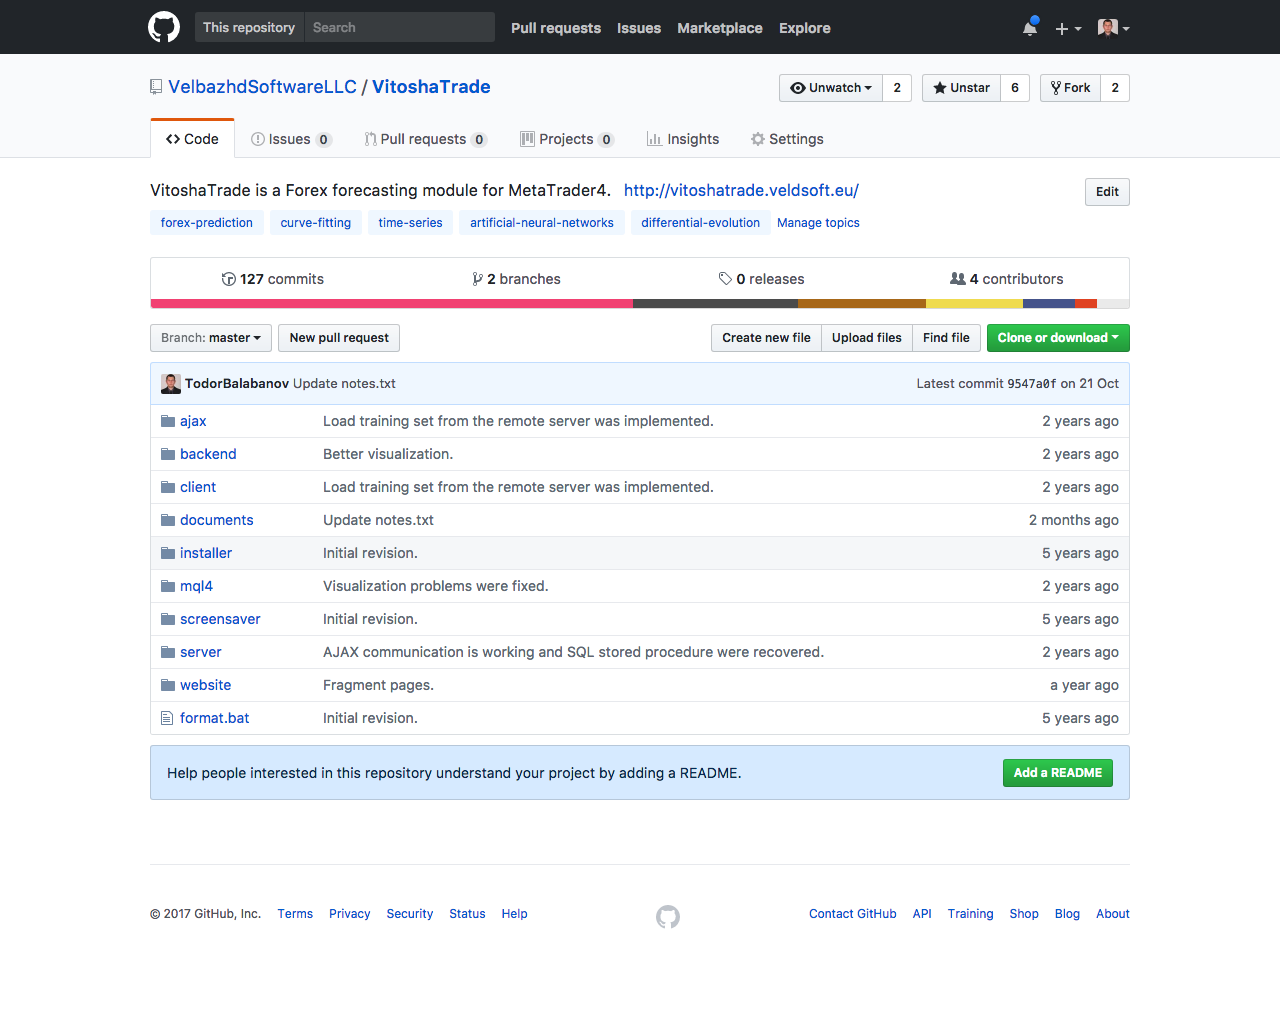
\includegraphics[height=0.45\pdfpageheight]{pic0095}
  \caption{Публично хранилище за кода на сървър приложението}
\label{fig:pic0095}
\end{figure}
\FloatBarrier

\section{Релационна база данни}

За нуждите от съхраняването на информация от страна на сървъра, е достатъчно да се разработи база от данни, в която таблиците са нормализирани поне до трета нормална форма (Фиг. \ref{fig:pic0096}).

\begin{figure}[h]
  \centering
  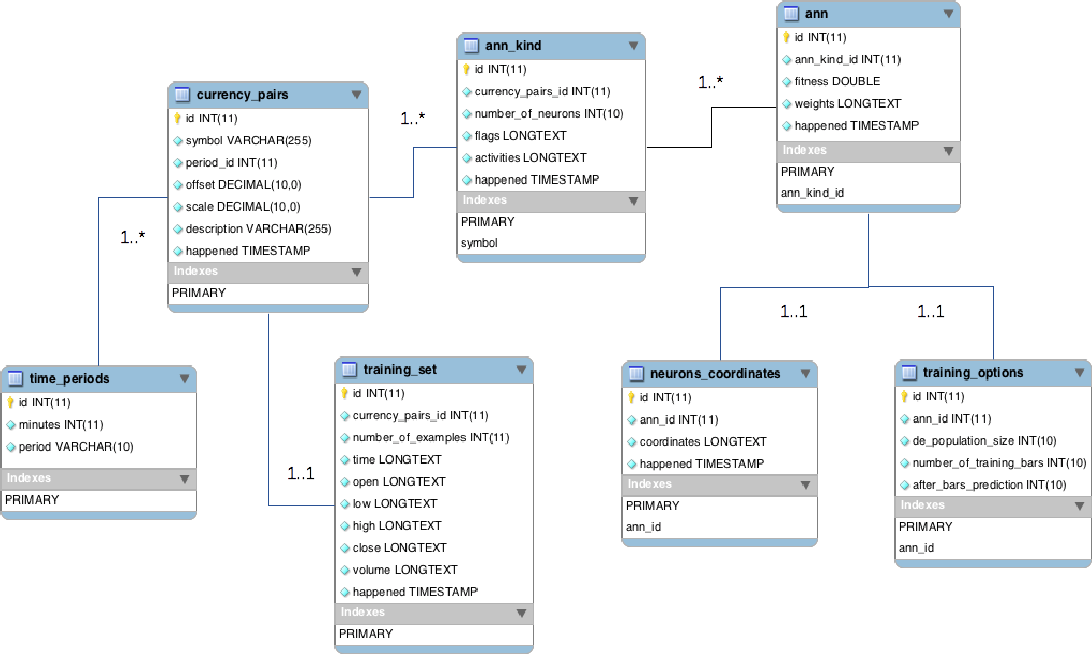
\includegraphics[height=0.35\pdfpageheight]{pic0096}
  \caption{Физическа структура на базата данни}
\label{fig:pic0096}
\end{figure}
\FloatBarrier

Това, което всеки един финансов времеви ред има, е интервал на който се извършват отчитанията на нивата. Тази информация се записва в таблица с три колони - служебен идентификатор, брой минути за интервала и символно название на интервала (Фиг. \ref{fig:pic0097}).

\begin{figure}[h]
  \centering
  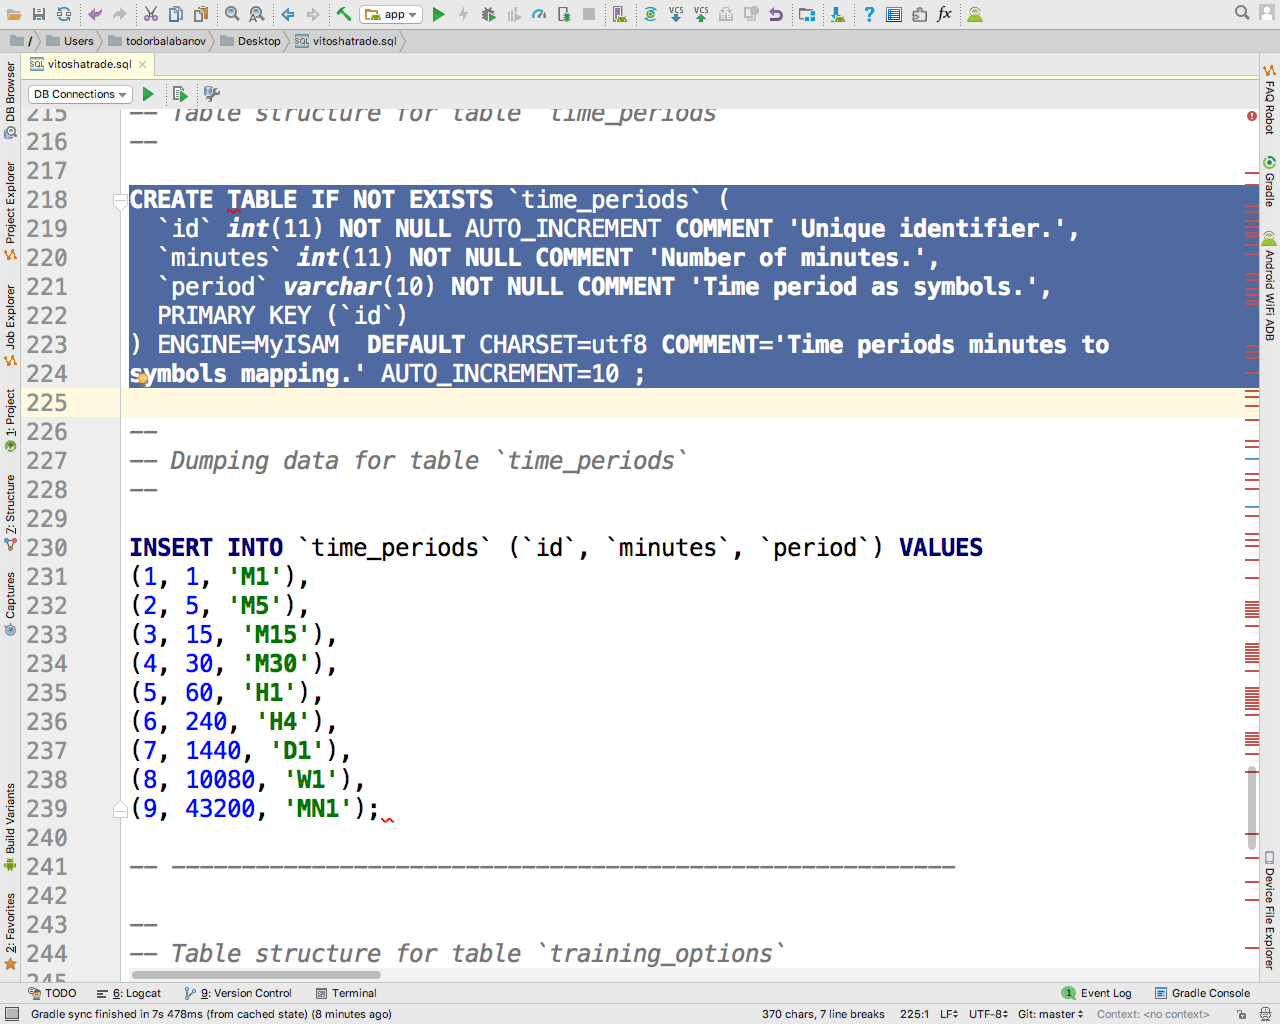
\includegraphics[height=0.45\pdfpageheight]{pic0097}
  \caption{Таблица с времевите интервали за редовете}
\label{fig:pic0097}
\end{figure}
\FloatBarrier

Най-съществената таблица в базата данни е таблицата за описване на валутните двойки (Фиг. \ref{fig:pic0098}). Тя съдържа следните полета - служебен идентификатор, название на валутната двойка, външен ключ към времевия интервал, отместване, необходимо за нормализиране на информацията, множител за мащабиране, също необходим за нормализирането на информацията, описание на валутната двойка и маркер за време, в което е направен записът в таблицата. 

\begin{figure}[h]
  \centering
  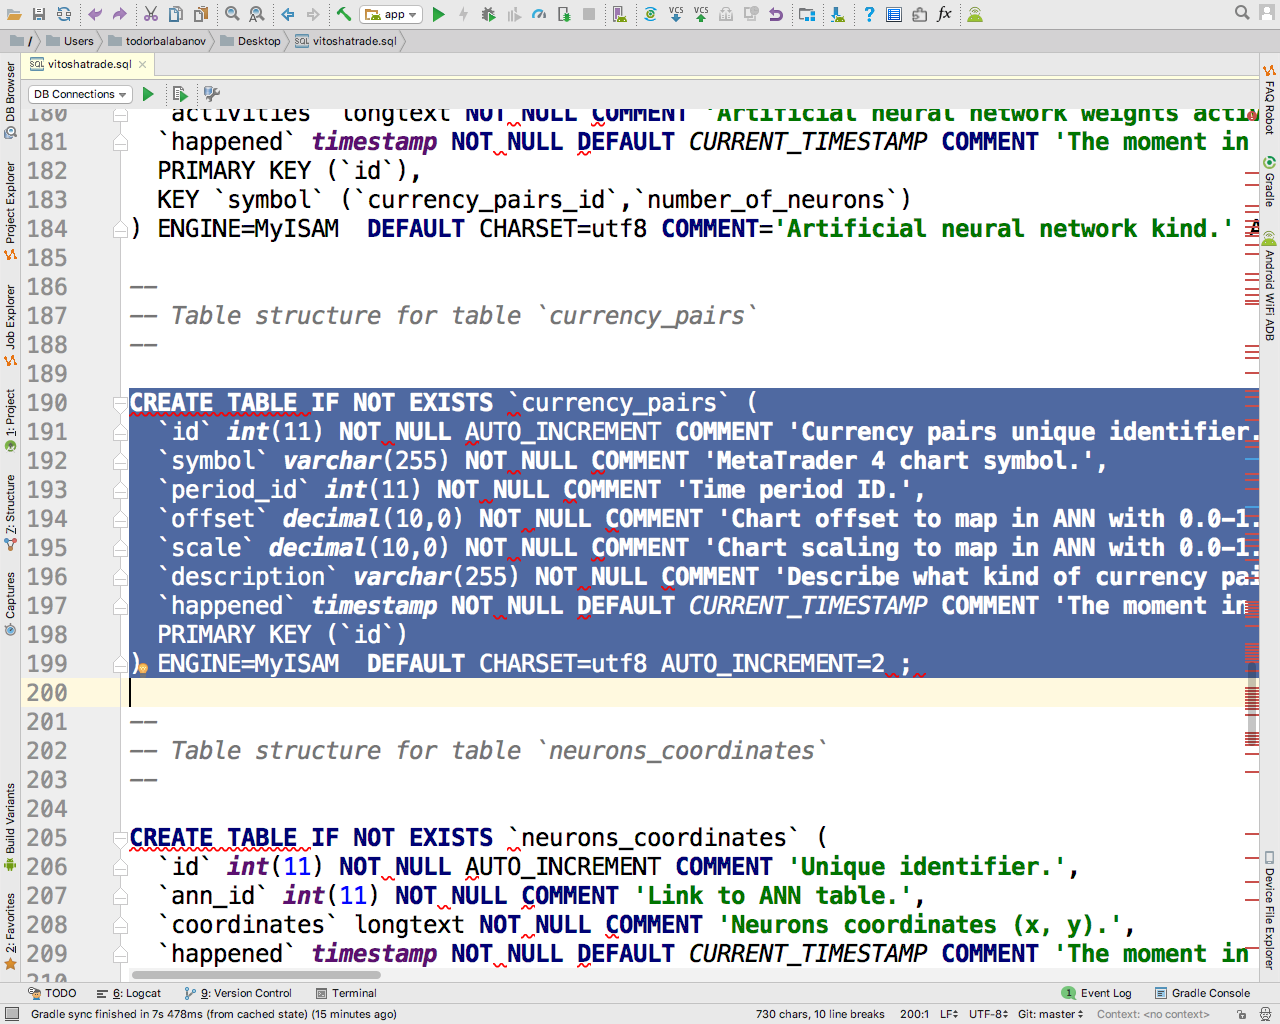
\includegraphics[height=0.45\pdfpageheight]{pic0098}
  \caption{Таблица за представяне на валутните двойки}
\label{fig:pic0098}
\end{figure}
\FloatBarrier

Топологията на всяка невронна мрежа се описва само един път в таблица за видовете мрежи (Фиг. \ref{fig:pic0099}). Тази таблица съдържа следните полета - служебен идентификатор, външен ключ към валутната двойка, за която се отнася мрежата, брой неврони, флагове за типа на невроните, стойности за връзките между невроните (според матрицата за съседство) и в кой момент от времето е направен записът в таблицата. 

\begin{figure}[h]
  \centering
  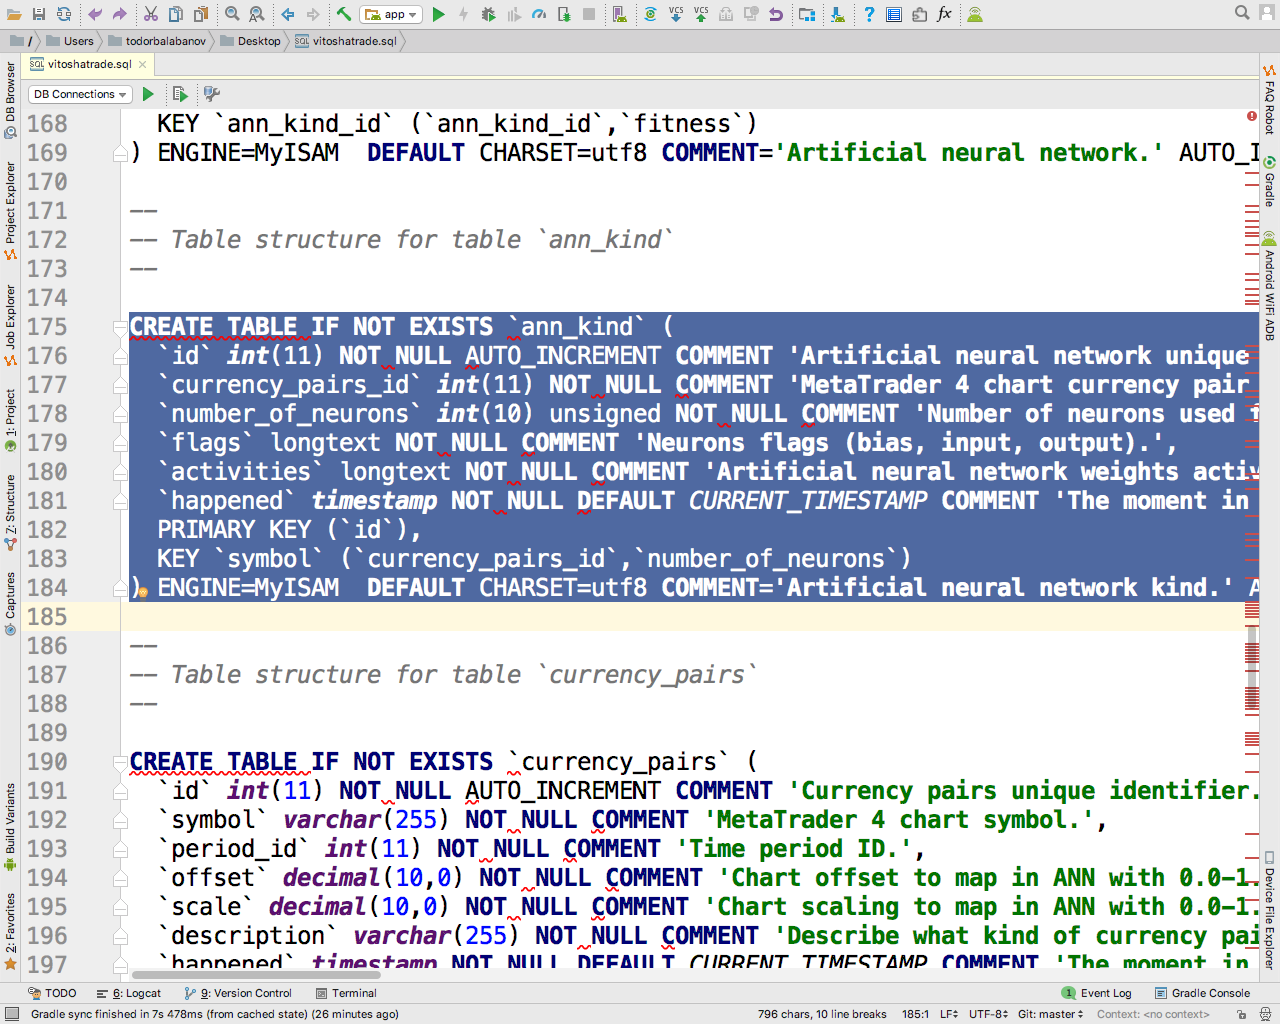
\includegraphics[height=0.45\pdfpageheight]{pic0099}
  \caption{Таблица за представяне на типовете мрежи}
\label{fig:pic0099}
\end{figure}
\FloatBarrier

На всяка топология мрежа може да отговарят множество екземпляри от тип изкуствена невронна мрежа (Фиг. \ref{fig:pic0100}). Информацията в таблицата за екземплярите е организирана в следните колони - служебен идентификатор, външен ключ към типа мрежа за който се отнася екземплярът, жизнена стойност на екземпляра, тегла на връзките между невроните (по графа за съседство) и момент от времето, в който е направен записът в таблицата. 

\begin{figure}[h]
  \centering
  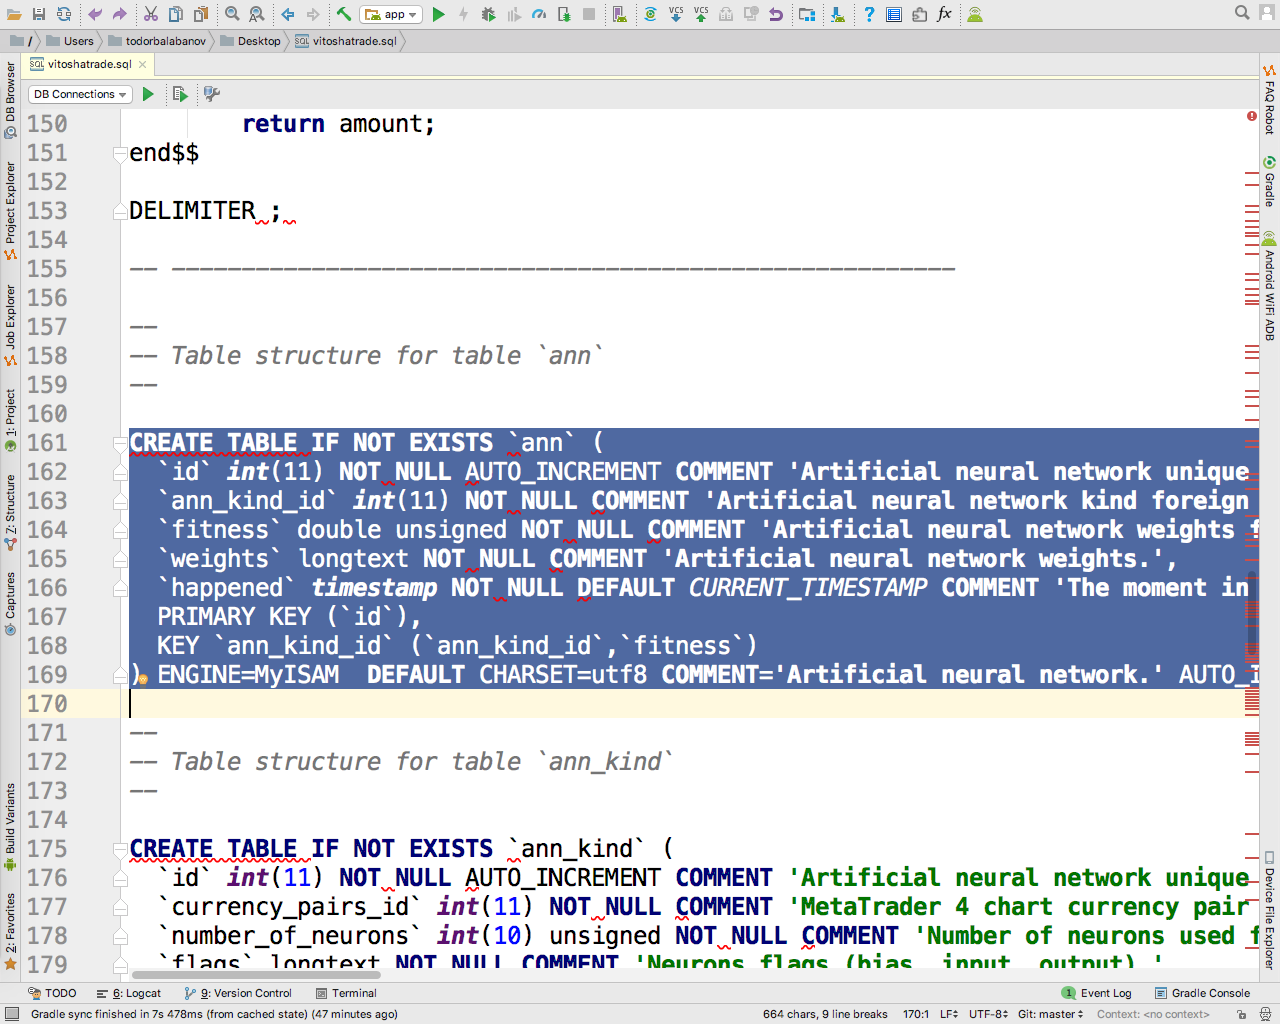
\includegraphics[height=0.45\pdfpageheight]{pic0100}
  \caption{Таблица за представяне на типовете мрежи}
\label{fig:pic0100}
\end{figure}
\FloatBarrier

За всеки екземпляр на невронна мрежа, е важно да се знае при какви параметри протича обучението му (Фиг. \ref{fig:pic0101}). За тази цел е предназначена отделна таблица със следните колони - служебен идентификатор, външен ключ към екземпляра, размер на популацията (когато става въпрос за обучаващ генетичен алгоритъм), брой барове на входа и брой барове на изхода.

\begin{figure}[h]
  \centering
  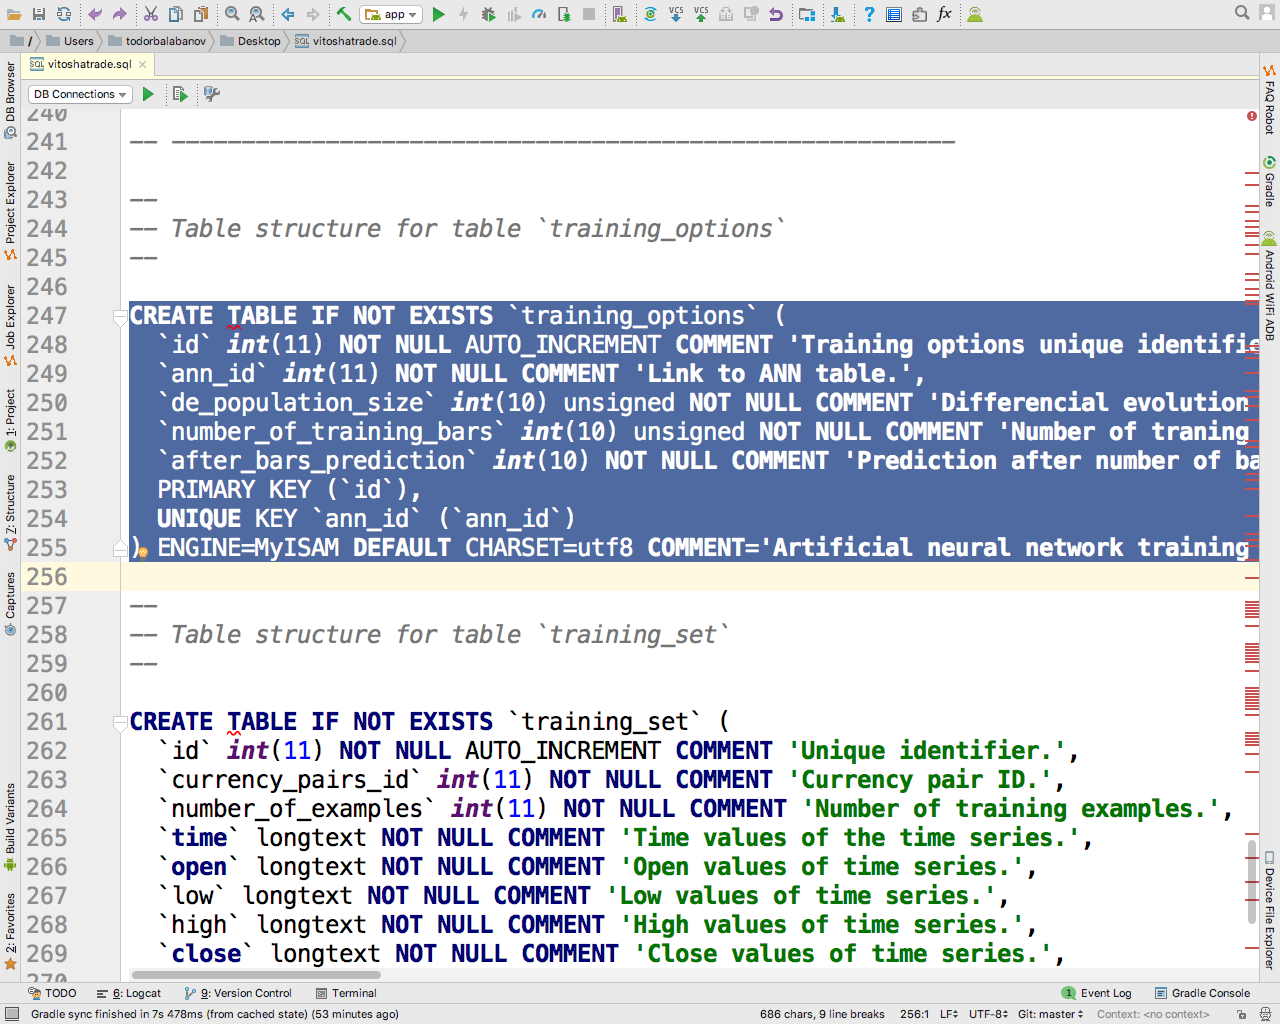
\includegraphics[height=0.45\pdfpageheight]{pic0101}
  \caption{Таблица с опции за протичане на обучението}
\label{fig:pic0101}
\end{figure}
\FloatBarrier

При нужда от визуално представяне на екземпляра за изкуствена невронна мрежа, е удачно да се съхранява информация за координатите на всеки неврон в равнината xOy (Фиг. \ref{fig:pic0102}). Тази таблица съдържа следните колони - служебен идентификатор, външен ключ към екземпляра, координати на невроните по реда на тяхното срещане в екземпляра и маркер за времето, в което е направен записът в таблицата. 

\begin{figure}[h]
  \centering
  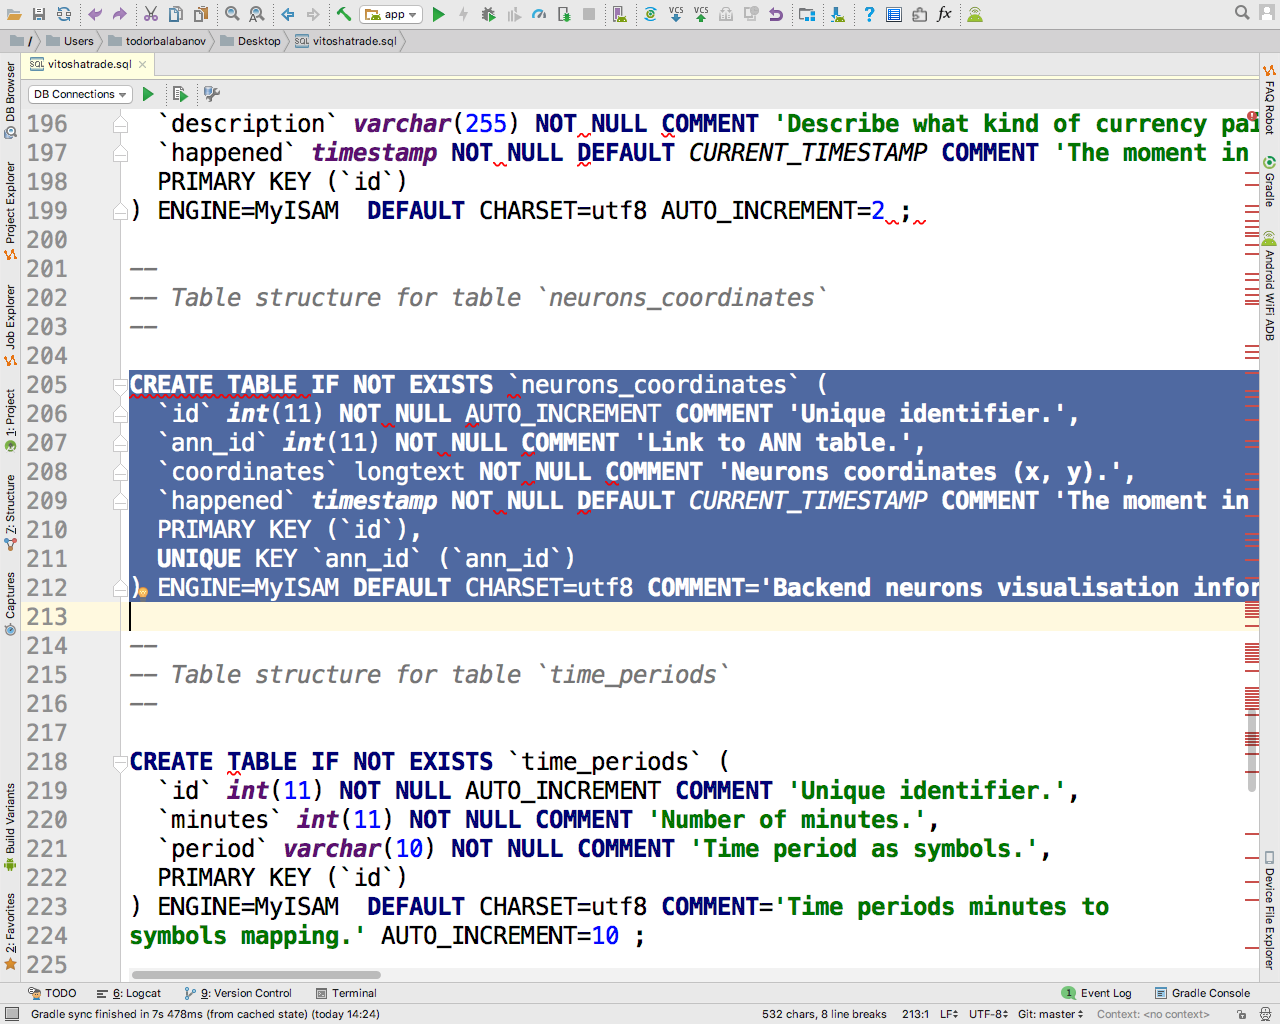
\includegraphics[height=0.45\pdfpageheight]{pic0102}
  \caption{Таблица с опции за протичане на обучението}
\label{fig:pic0102}
\end{figure}
\FloatBarrier

Последната, но изключително важна таблица, е таблицата за съхранение на обучаващите примери, съдържащи информацията за финансовия времеви ред (Фиг. \ref{fig:pic0103}). Тази таблица съдържа следните колони - служебен идентификатор, външен ключ към валутната двойка, брой измервания, последователност от времеви маркери, последователност от нива (отваряне, най-ниско, най-високо, затваряне), търгуван обем и времеви маркер за момента, в който е направен записът в таблицата. 

\begin{figure}[h]
  \centering
  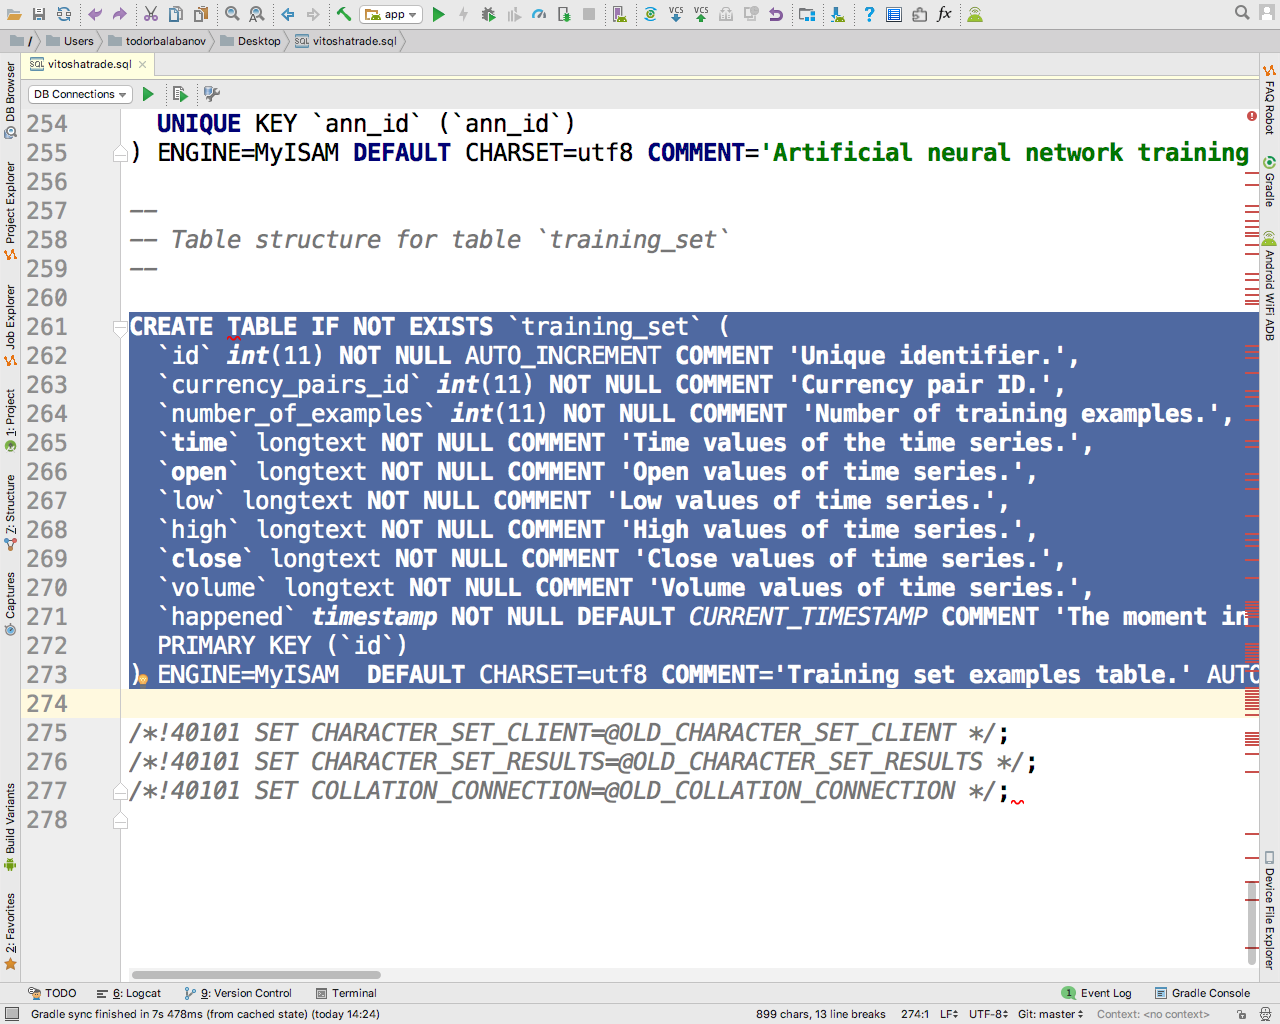
\includegraphics[height=0.45\pdfpageheight]{pic0103}
  \caption{Таблица с опции за протичане на обучението}
\label{fig:pic0103}
\end{figure}
\FloatBarrier

\section{Алгоритмична обработка на суровите данни}

За да се постигне добро разделяне, според трислойната архитектура на системата, от съществено значение е суровите данни да бъдат минимално обвързани с работната логика. Често срещана практика е смесването на работата със суровите данни и програмния код от работната логика. Такова смесване лесно се получава, ако в скриптовете от работната логика се изпълняват сложни SQL заявки. Подобен начин за конструиране на сървърното приложение прави системата трудна за поддържане и още по-трудна за реорганизиране, ако се наложи смяна на системата за управление на бази от данни или инструментите използвани в слоя на работната логика. Добро разделяне между двата слоя се получава, когато работната логика, под формата на SQL заявки, единствено вика съхранени функции и процедури (stored procedures) на системата за управление на бази от данни. От една страна синтаксисът на заявките в междинния слой става максимално опростен, от друга страна евентуална подмяна на базата данни би довела до единствена корекция в начина, по който се извикват съхранените функции и процедури. За да се удовлетвори стремежът за максимално разделяне между слоевете, към структурата на базата данни са добавени група съхранени функции и процедури. 

\begin{figure}[h]
  \centering
  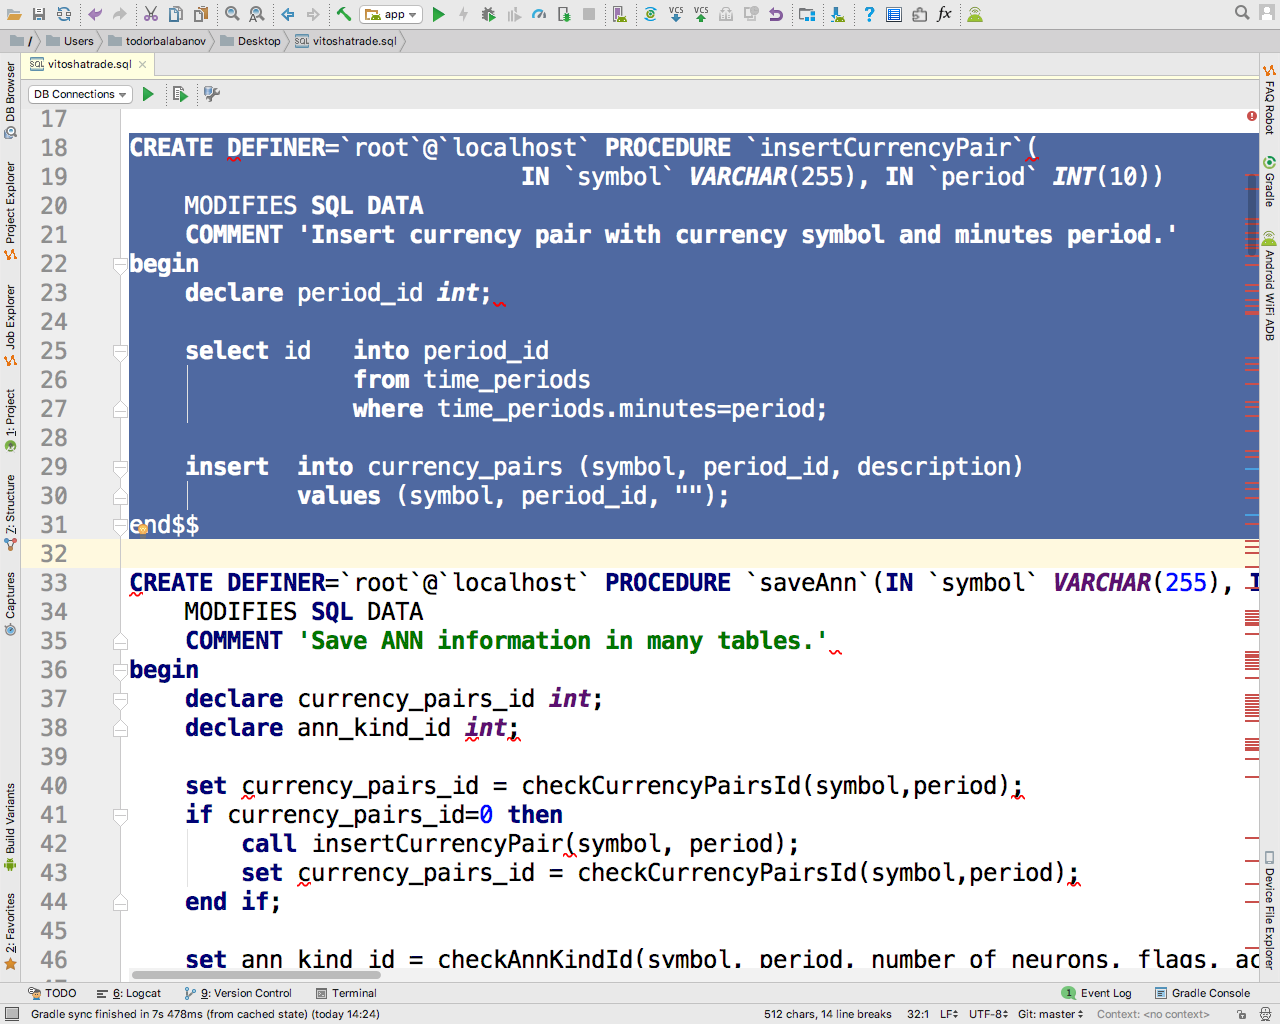
\includegraphics[height=0.45\pdfpageheight]{pic0104}
  \caption{Процедура за добавяне на валутна двойка}
\label{fig:pic0104}
\end{figure}
\FloatBarrier

При добавянето на нова валутна двойка, като входни данни постъпват названието на валутната двойка и времевият интервал (в брой минути), който интервал трябва да бъде съпоставен на интервалите, изброени в таблицата с времеви интервали. Това налага използването на съхранена процедура, която да извърши обработката на входната информация (Фиг. \ref{fig:pic0104}). 

\begin{figure}[h]
  \centering
  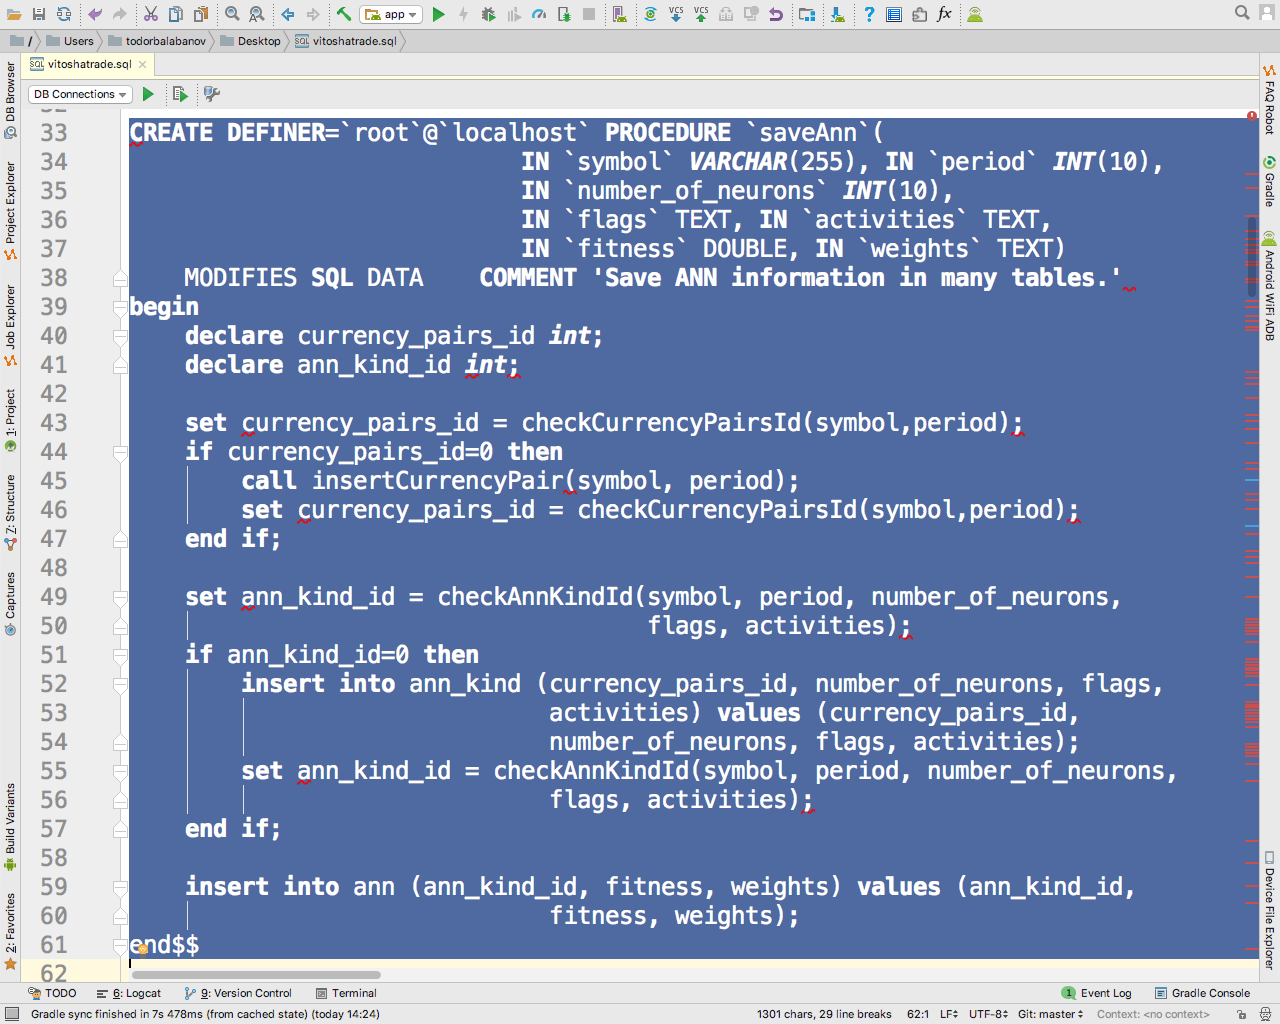
\includegraphics[height=0.45\pdfpageheight]{pic0105}
  \caption{Процедура за запис на екземпляр от изкуствена невронна мрежа}
\label{fig:pic0105}
\end{figure}
\FloatBarrier

При записването на екземпляр от изкуствена невронна мрежа, към базата данни постъпва информация за валутната двойка, периода на времевия ред, броя и типовете на невроните, матрици на съседство за връзките и жизнена оценка на екземпляра (Фиг. \ref{fig:pic0105}). Преди екземплярът да бъде добавен в таблицата с екземплярите се проверява дали валутната дойка е налична и се определя нейният идентификатор. Ако валутната двойка не е налична, то тя се създава. Следва проверка за съществуването на типа мрежа. Ако не съществува, то тя се създава. Последната инструкция е самото добавяне на екземпляра към таблицата с екземплярите. При така подбраната стратегия за работа максимално се спазват правилата за съблюдаване на референциалния интегритет. 

\begin{figure}[h]
  \centering
  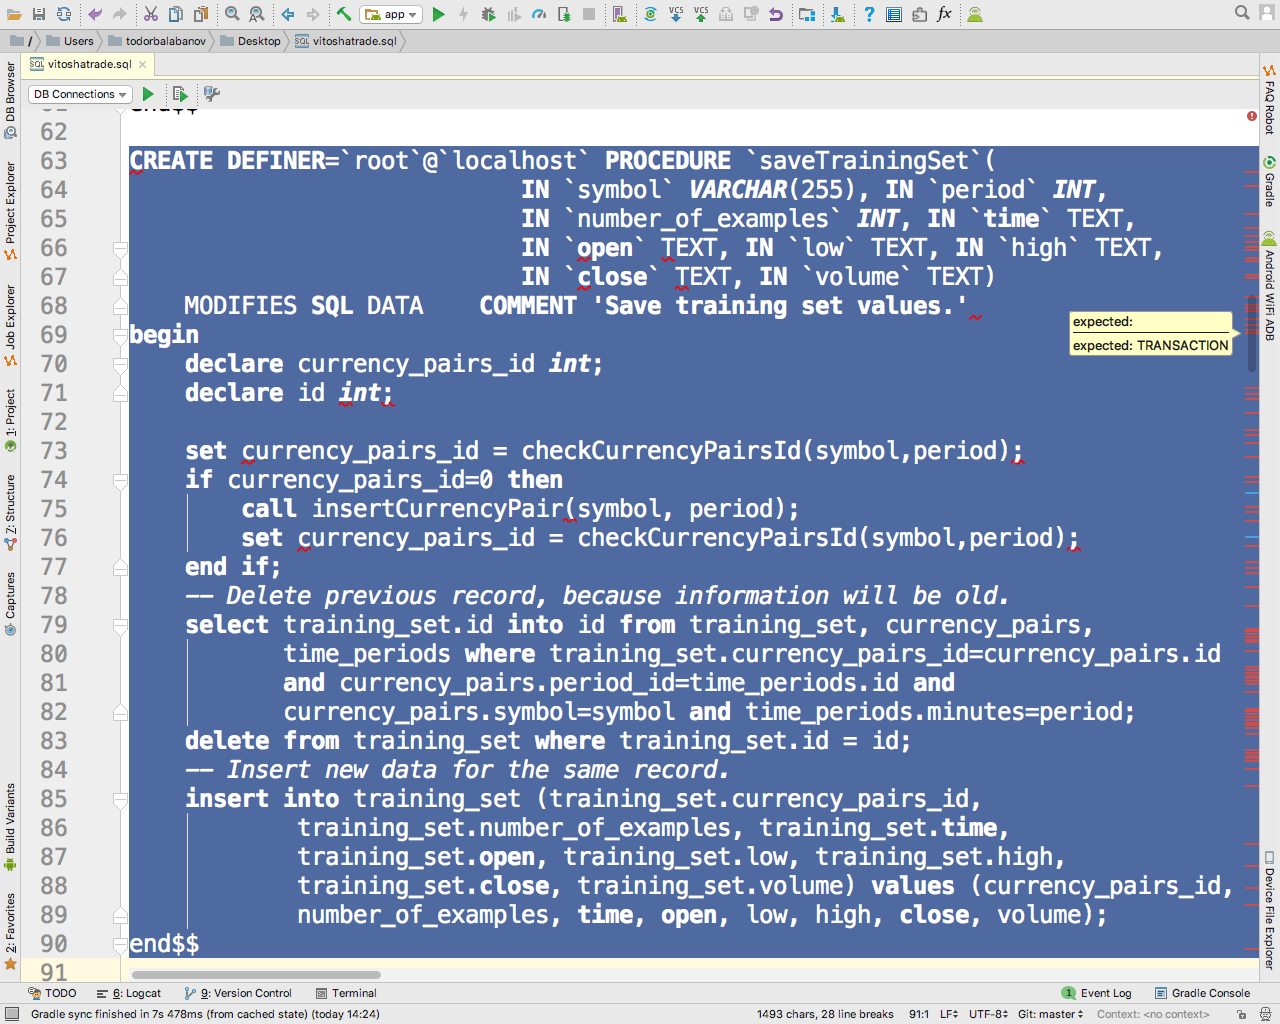
\includegraphics[height=0.45\pdfpageheight]{pic0106}
  \caption{Процедура за запис на тренировъчни примери}
\label{fig:pic0106}
\end{figure}
\FloatBarrier

При записа на тренировъчни примери, на входа на базата данни се подават серия параметри за стойностите на времевия ред (Фиг. \ref{fig:pic0106}). По аналогичен начин се извършва проверка за съществуване на валутната двойка. Следва изтриване на предишни тренировъчни примери, ако такива бъдат открити. Финалната стъпка е добавянето на постъпилата информация. 

\begin{figure}[h]
  \centering
  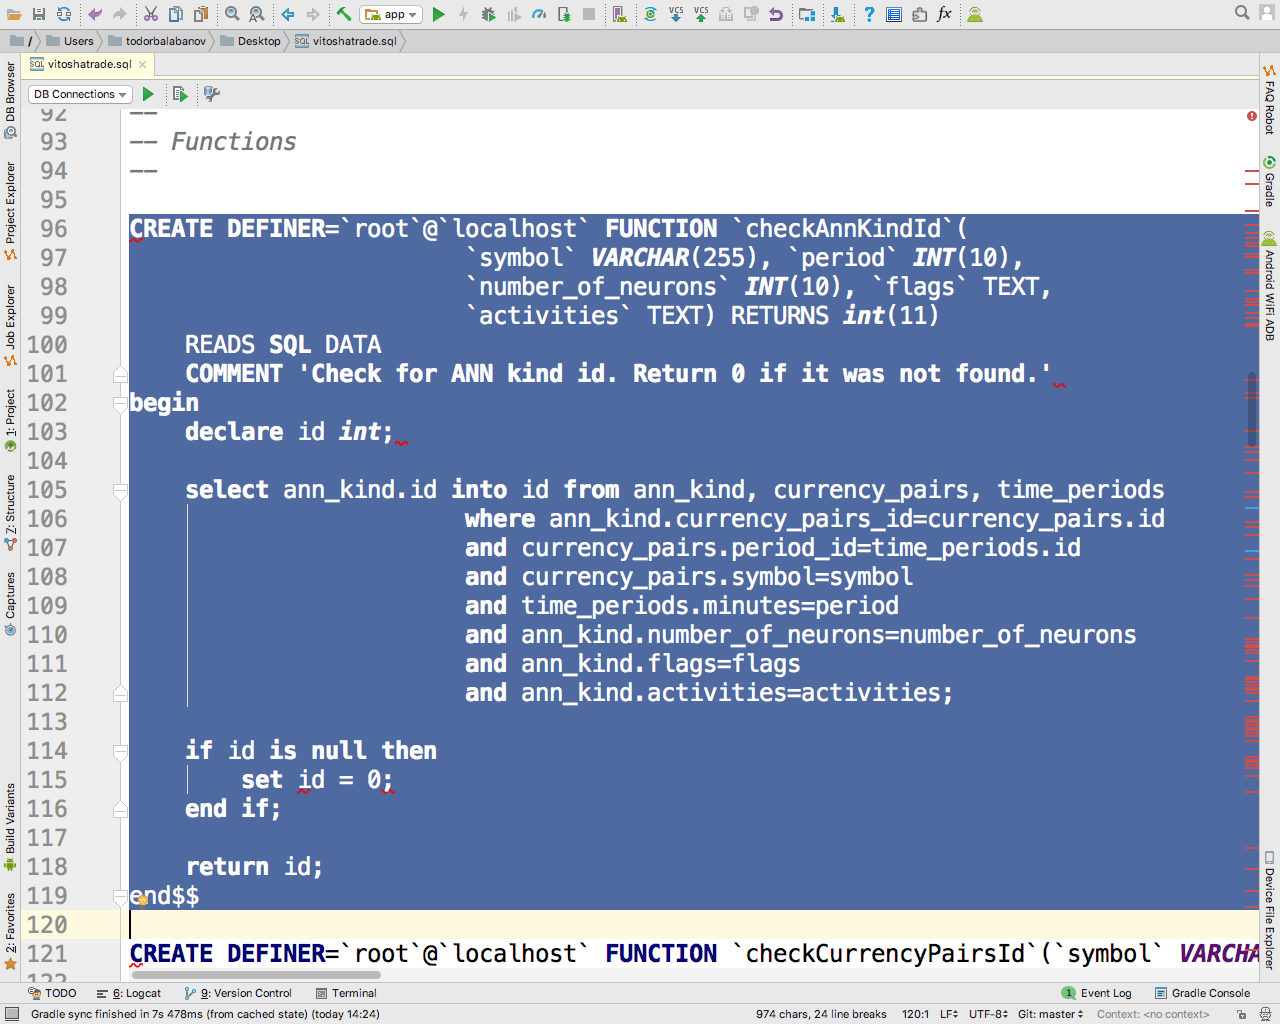
\includegraphics[height=0.45\pdfpageheight]{pic0107}
  \caption{Функция за определяне на типа мрежа}
\label{fig:pic0107}
\end{figure}
\FloatBarrier

Помощна функция определя служебния идентификатор на типа мрежа по описанието на екземпляр (Фиг. \ref{fig:pic0107}). Ако не бъде открит такъв тип служебно се връща нулева стойност. 

\begin{figure}[h]
  \centering
  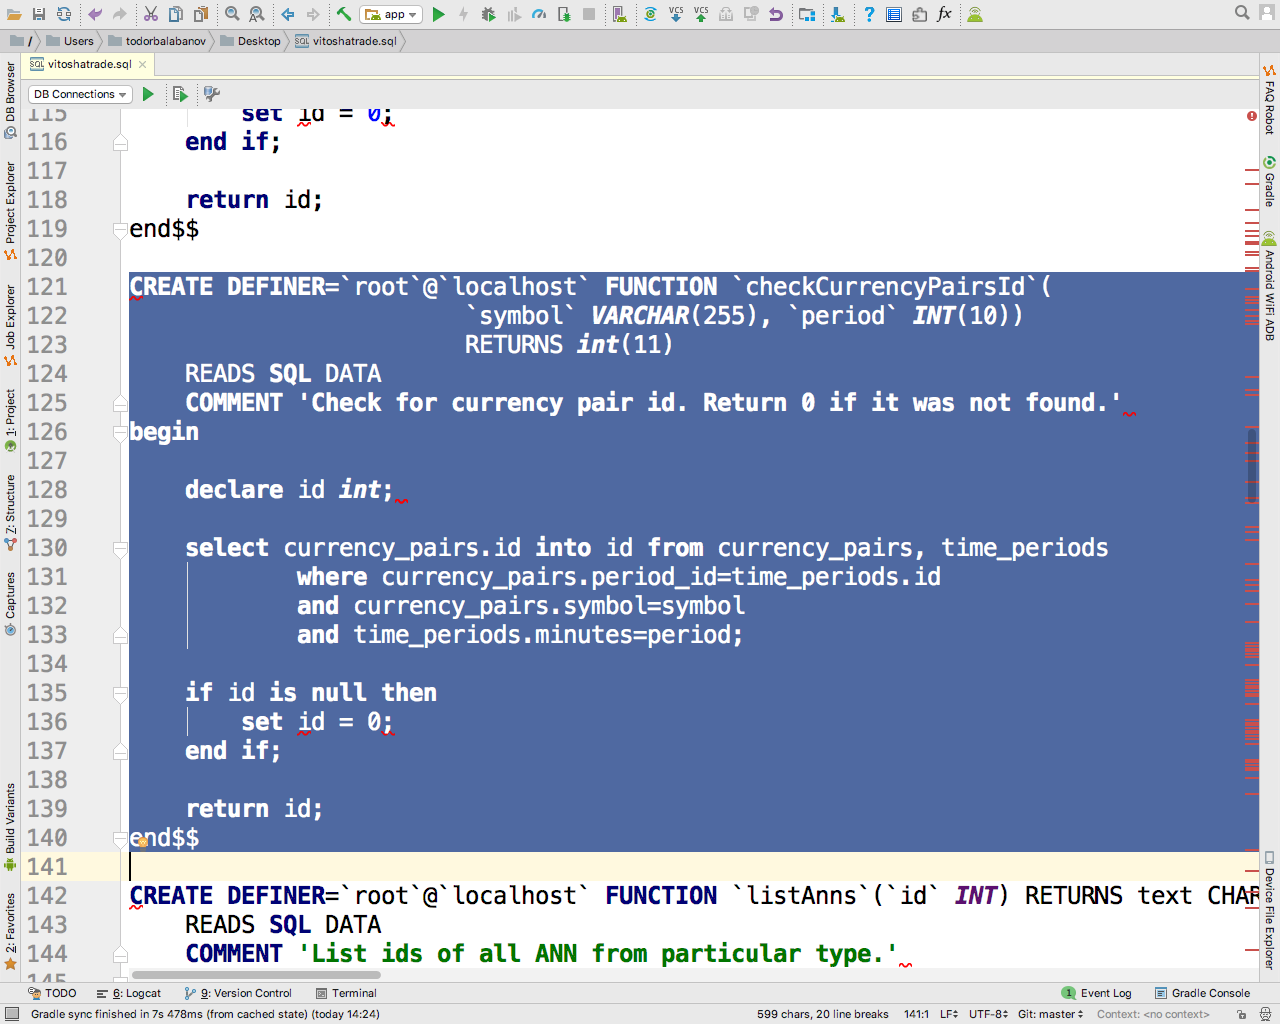
\includegraphics[height=0.45\pdfpageheight]{pic0108}
  \caption{Функция за определяне на типа валутна двойка}
\label{fig:pic0108}
\end{figure}
\FloatBarrier

По аналогичен начин, помощна функция служи за определяне на служебния идентификатор за валутна двойка, чрез зададено символно име и период (Фиг. \ref{fig:pic0108}). Ако валутната двойка не бъде открита се връща служебна нула. 

\begin{figure}[h]
  \centering
  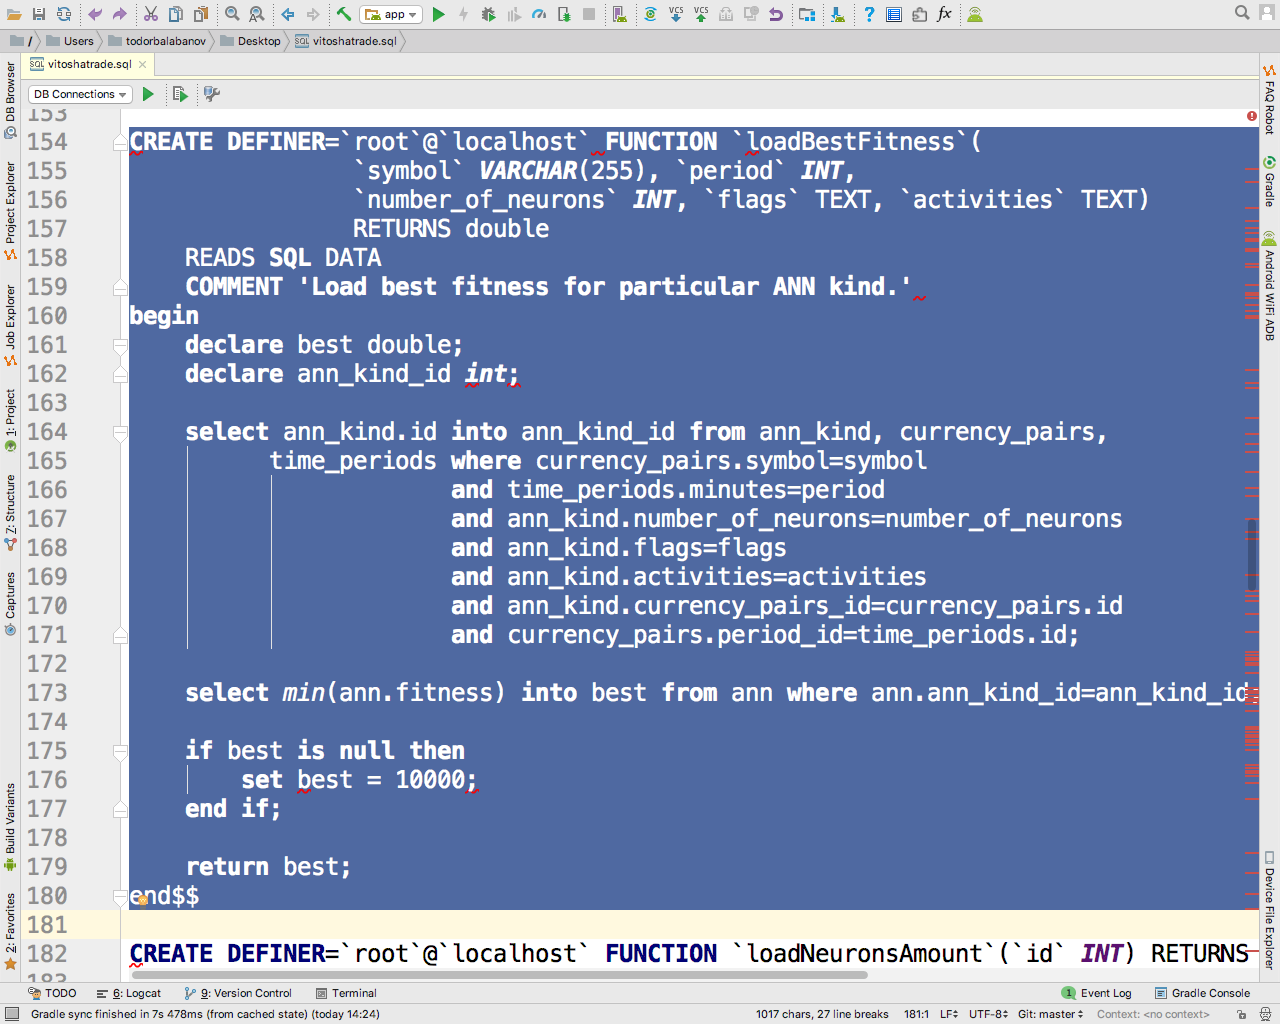
\includegraphics[height=0.45\pdfpageheight]{pic0109}
  \caption{Функция за определяне на най-добрата жизненост}
\label{fig:pic0109}
\end{figure}
\FloatBarrier

По зададено описание на изкуствена невронна мрежа, клиентските мобилни устройства запитват сървъра, на определени интервали от време, колко е стойността на най-жизнената мрежа. Това запитване е съществено, тъй като по него се взема решение дали мобилното устройство да докладва резултатите си на сървъра. Обработката се извършва на две стъпки - първо се намират всички мрежи с идентична топология, а след това се определя най-добрата жизненост (Фиг. \ref{fig:pic0109}).

\begin{figure}[h]
  \centering
  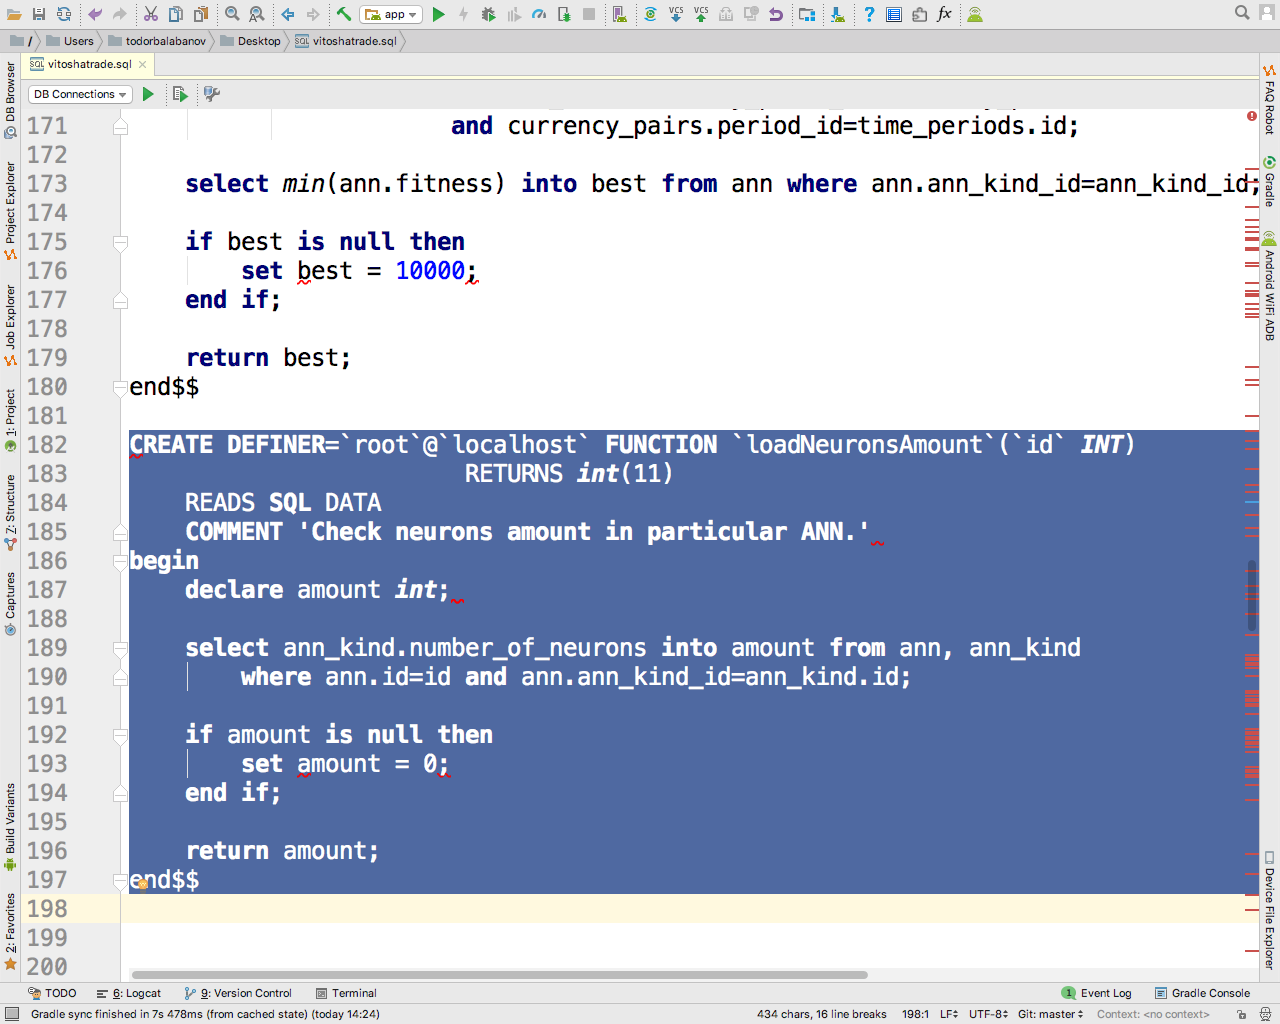
\includegraphics[height=0.45\pdfpageheight]{pic0110}
  \caption{Функция за определяне на броя неврони за определен еземпляр мрежа}
\label{fig:pic0110}
\end{figure}
\FloatBarrier

Помощна функция определя и броя неврони по зададен идентификатор на екземпляр мрежа (Фиг. \ref{fig:pic0110}).

\section{Сървър скриптове}

Директният достъп до базата данни (TCP свързване) често е нежелателен, тъй като създава определени опасности за сигурността на данните. Поради тази причина е прието да се използва междинен слой, който да осъществява комуникацията с базата данни. За нуждите на настоящото помагало това са група PHP скриптове. 

\begin{figure}[h]
  \centering
  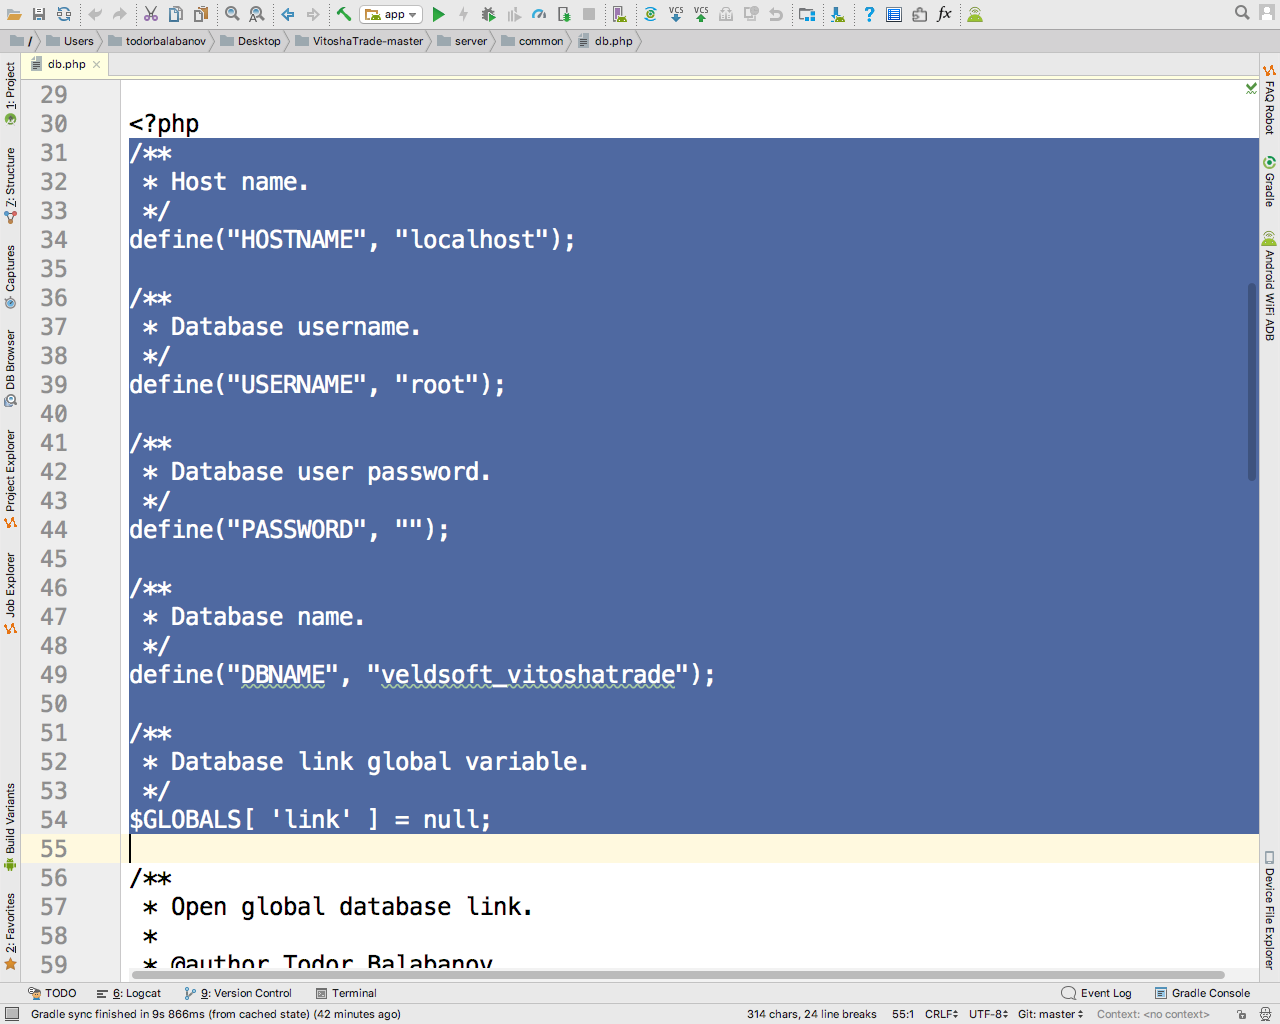
\includegraphics[height=0.45\pdfpageheight]{pic0111}
  \caption{Глобални променливи за достъп до базата данни}
\label{fig:pic0111}
\end{figure}
\FloatBarrier

В специално отделен за целта файл (db.php) се задават следните глобални променливи за достъп до базата данни - хост на който е разположен MySQL сървърът, потребител в MySQL, парола на потребителя, название на базата данни и връзка (Фиг. \ref{fig:pic0111}).

\begin{figure}[h]
  \centering
  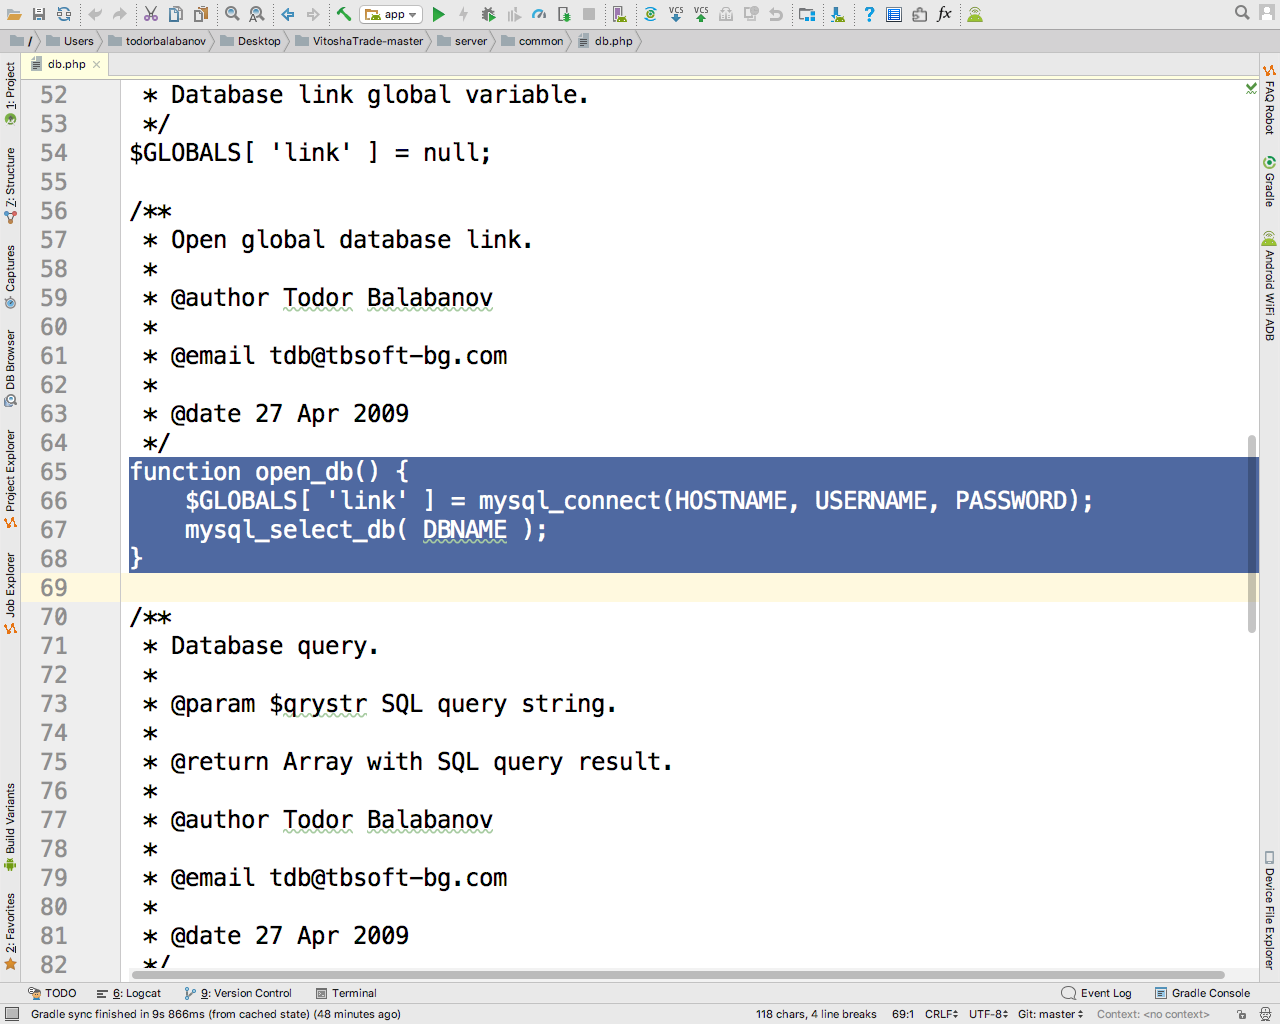
\includegraphics[height=0.45\pdfpageheight]{pic0112}
  \caption{Отваряне на връзка към базата данни}
\label{fig:pic0112}
\end{figure}
\FloatBarrier

Две помощни функции служат за отваряне и затваряне на връзка към базата данни (Фиг. \ref{fig:pic0112}, \ref{fig:pic0113}).

\begin{figure}[h]
  \centering
  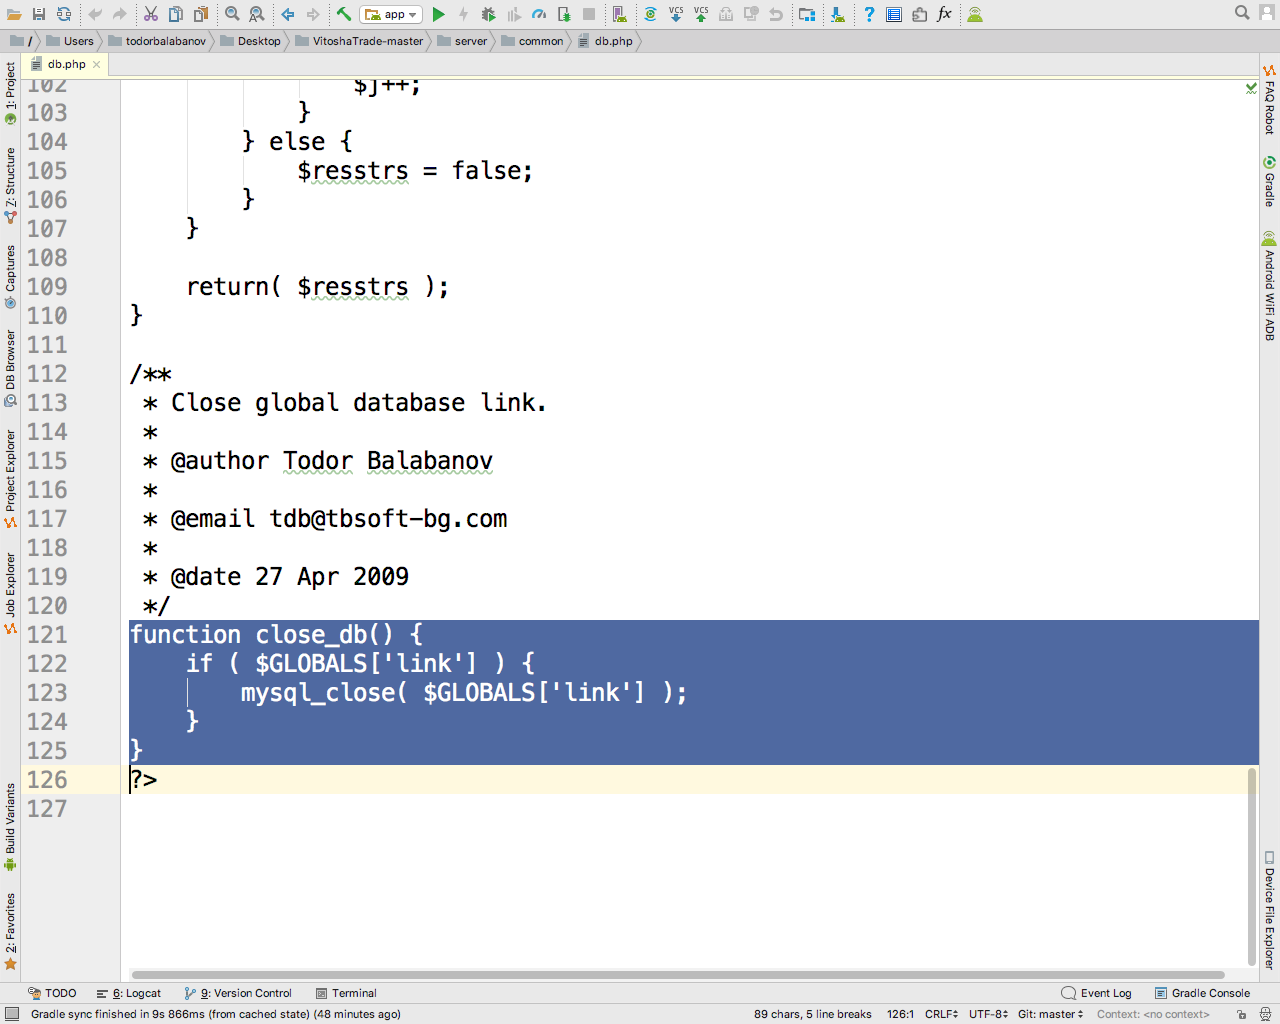
\includegraphics[height=0.45\pdfpageheight]{pic0113}
  \caption{Затваряне на връзката към базата данни}
\label{fig:pic0113}
\end{figure}
\FloatBarrier

Допълнителна помощна функция изпълнява заявките към базата данни и връща резултата от изпълнението под формата на двумерен масив (Фиг. \ref{fig:pic0114}).

\begin{figure}[h]
  \centering
  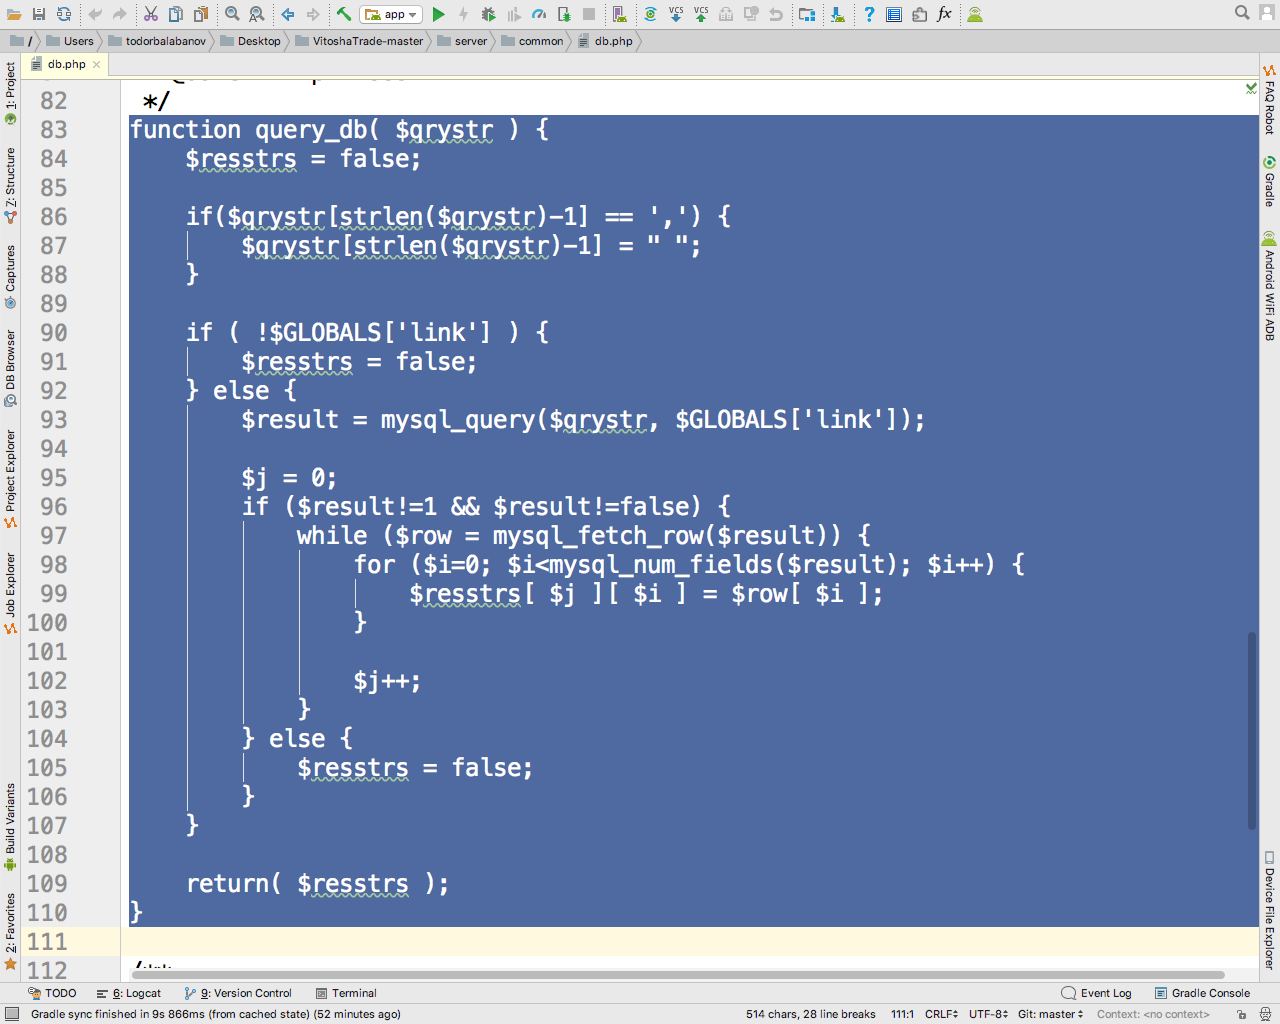
\includegraphics[height=0.45\pdfpageheight]{pic0114}
  \caption{Изпълнение на заявки към базата данни}
\label{fig:pic0114}
\end{figure}
\FloatBarrier

На този етап в разработката клиентското приложение изпраща своите данни под формата на POST заявка, а сървърът отговаря с JSON съобщение. Макар и спестяващ допълнителна работа около съставянето на JSON съобщения от страна на клиента, този подход не е за препоръчване и е желателно клиентите също да изпращат информацията в JSON формат, така че да се спазват конвенциите на RESTful приложенията. 

\subsection{Зареждане на мрежа по идентификатор}

Всеки екземпляр на изкуствена невронна мрежа има служебен идентификатор, който представлява и първичен ключ в съответната таблица. За да бъде заредена мрежата, се извиква PHP скрипт изпълняващ тази задача. 

\begin{figure}[h]
  \centering
  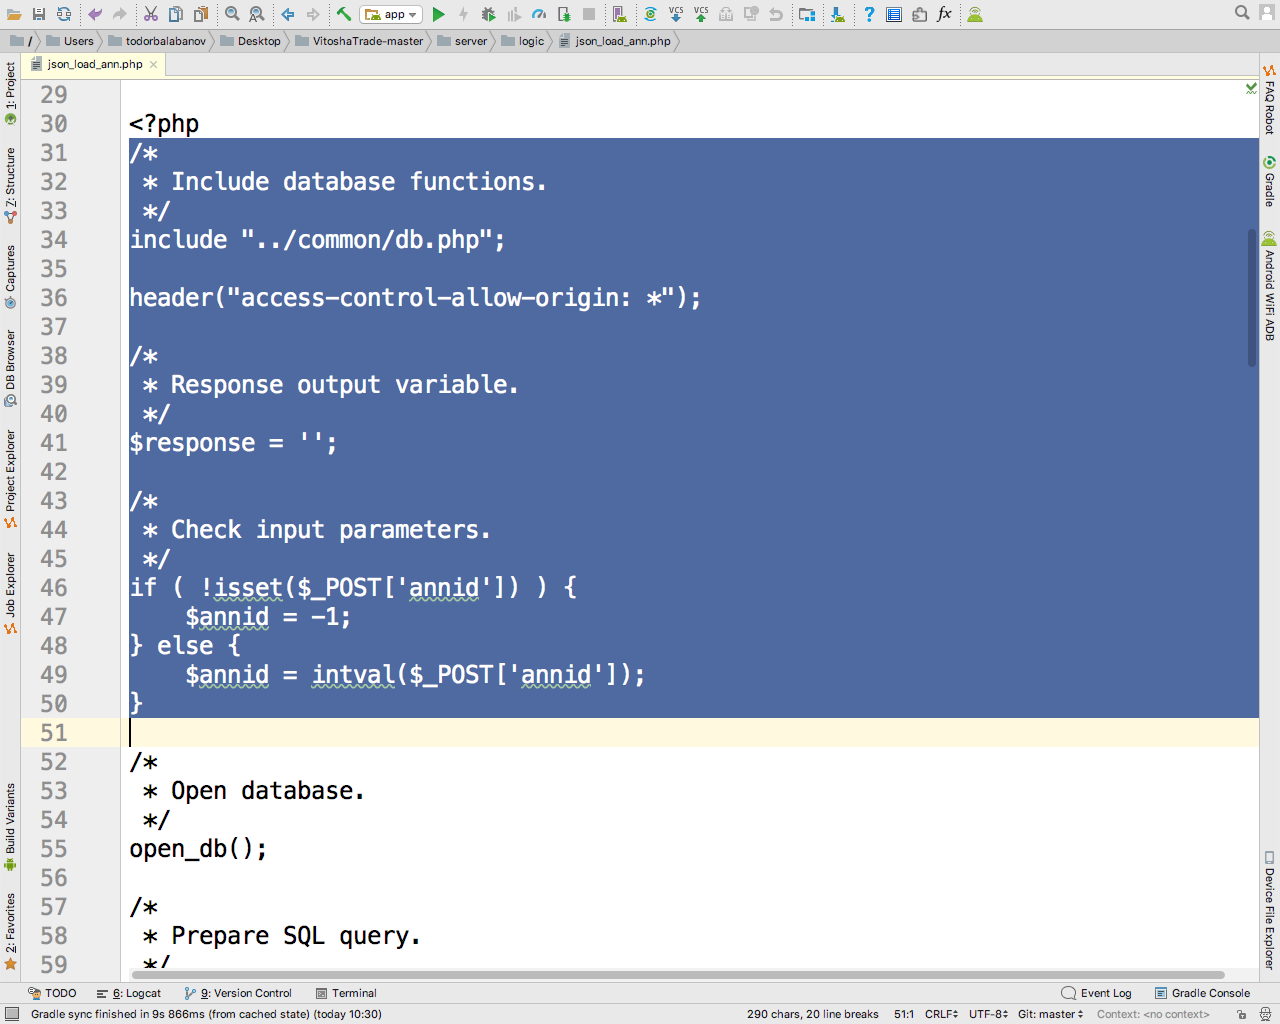
\includegraphics[height=0.45\pdfpageheight]{pic0115}
  \caption{Проверка на входните данни}
\label{fig:pic0115}
\end{figure}
\FloatBarrier

Преди същинското зареждане на мрежата се включва модулът за работа с базата данни и се извършва проверка на входните параметри. В случая единственият параметър е цяло число което е идентификатор на екземпляра (Фиг. \ref{fig:pic0115}).

\begin{figure}[h]
  \centering
  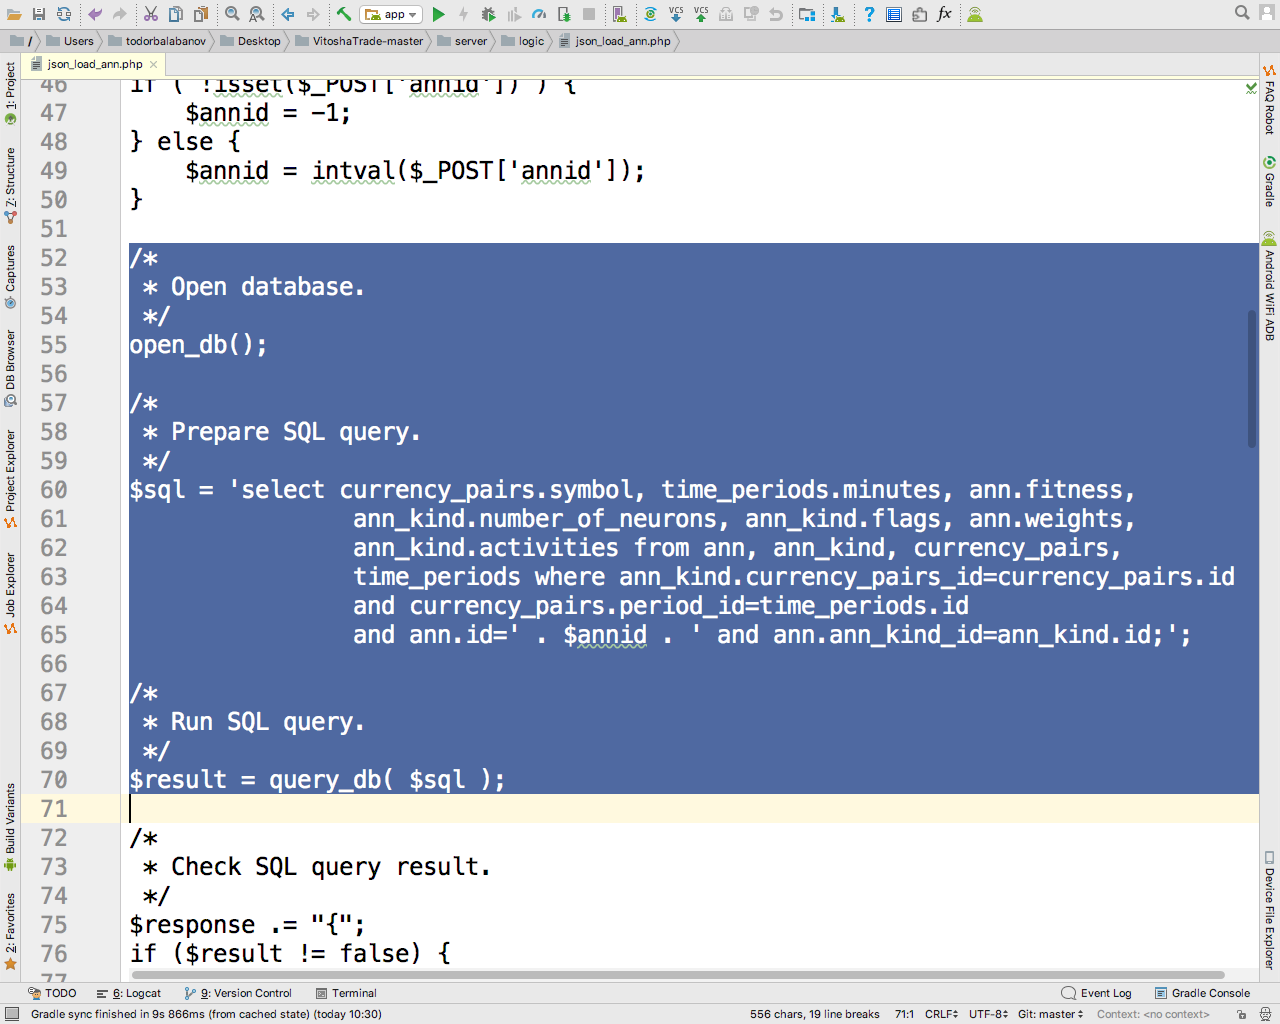
\includegraphics[height=0.45\pdfpageheight]{pic0116}
  \caption{Заявка за извличане на екземпляр по идентификатор}
\label{fig:pic0116}
\end{figure}
\FloatBarrier

Следва отваряне на връзка към базата данни, съставяне на заявка (добрата практика изисква извикване на съхранена функция) и изпълнение на заявката (Фиг. \ref{fig:pic0116}). 

\begin{figure}[h]
  \centering
  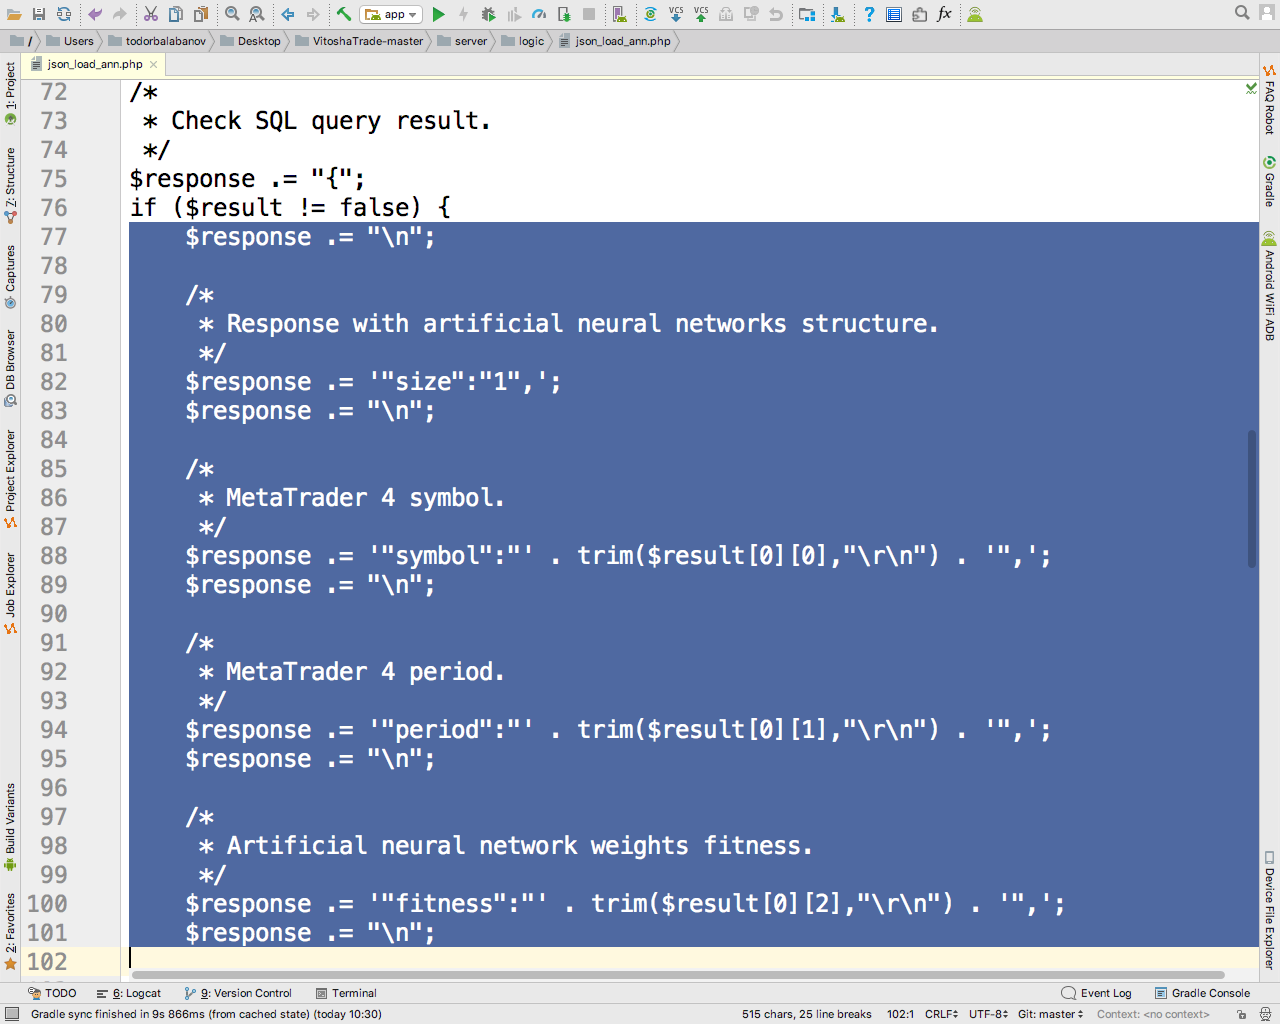
\includegraphics[height=0.45\pdfpageheight]{pic0117}
  \caption{Проверка за наличност на екземпляра}
\label{fig:pic0117}
\end{figure}
\FloatBarrier

Възможни са два изхода от изпълнението на заявката, спрямо това дали такъв екземпляр присъства в базата данни или не присъства. Ако екземплярът бъде открит започва изграждането на JSON съобщение с отговор към клиента. Отговорът съдържа единица, за намерен екземпляр, названието на валутната двойка, интервала на времевия ред, жизнената стойност на екземпляра, брой и типове на невроните, матрица на връзките и матрица на теглата (Фиг. \ref{fig:pic0117}-\ref{fig:pic0120}).

\begin{figure}[h]
  \centering
  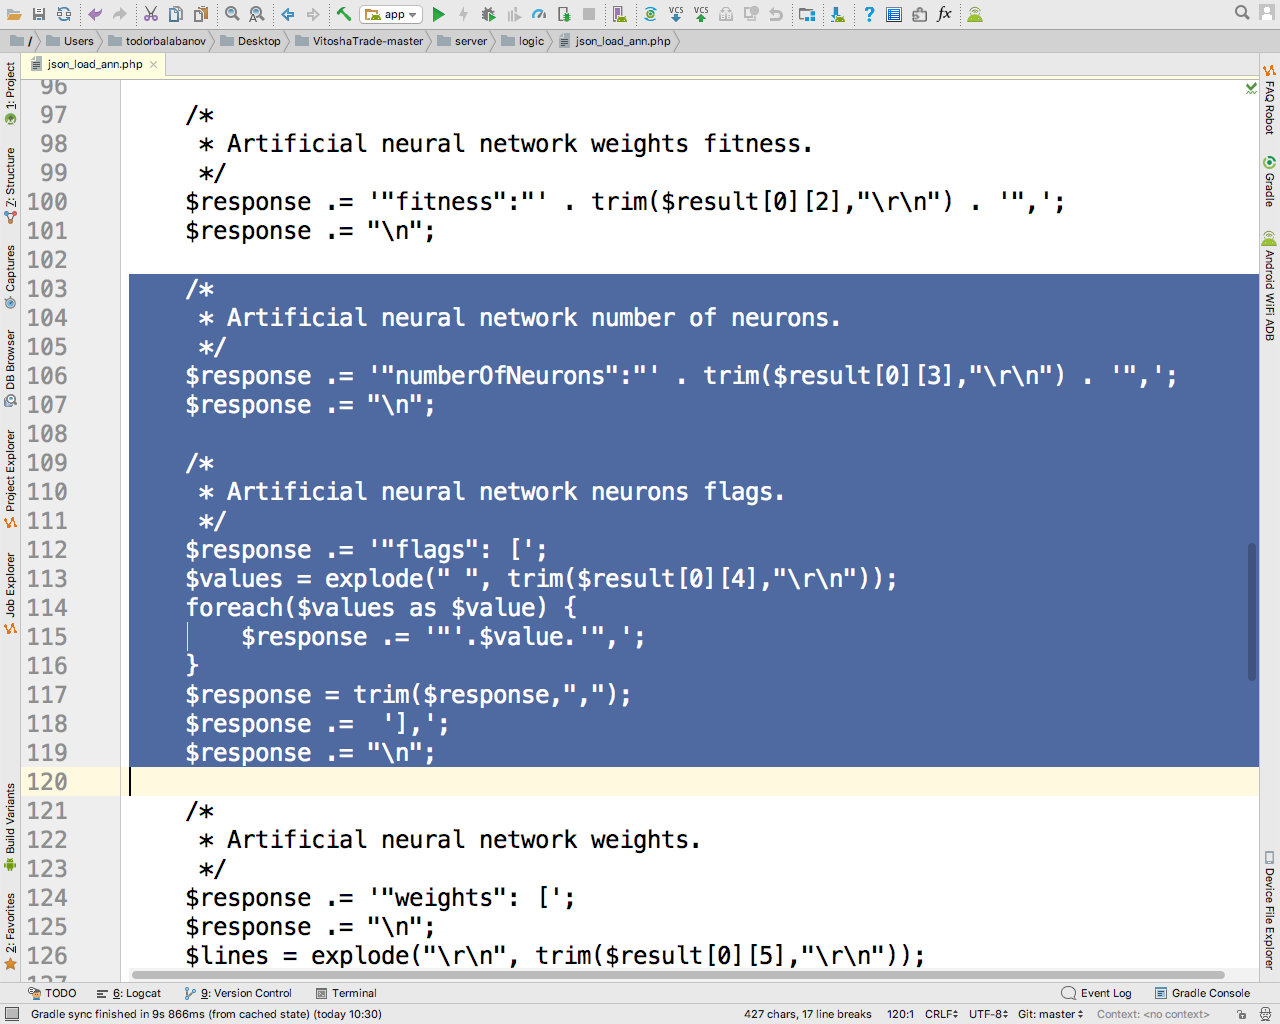
\includegraphics[height=0.45\pdfpageheight]{pic0118}
  \caption{Информация за невроните}
\label{fig:pic0118}
\end{figure}
\FloatBarrier

\begin{figure}[h]
  \centering
  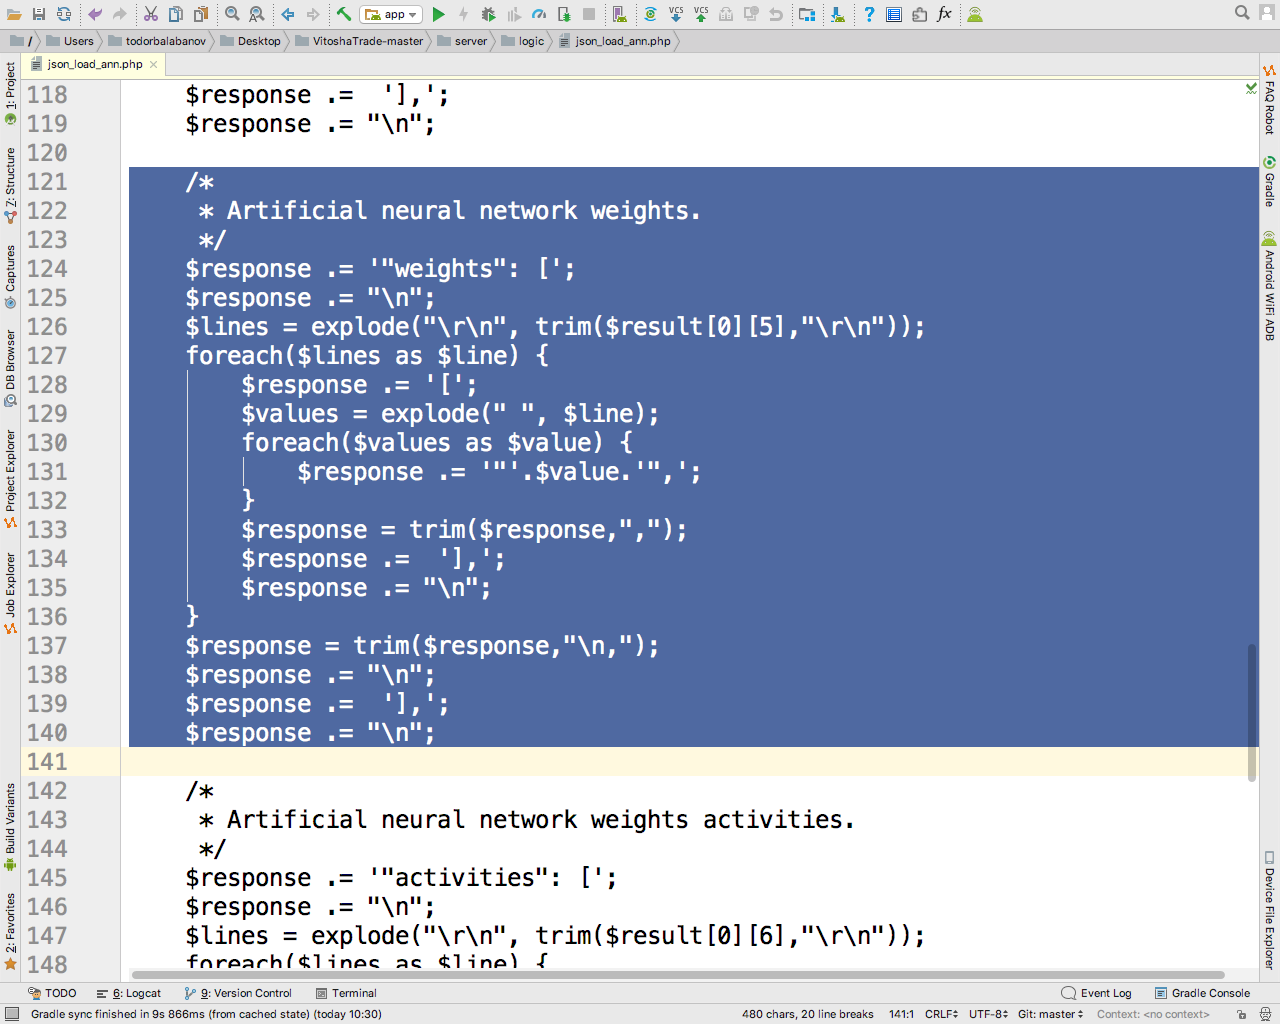
\includegraphics[height=0.45\pdfpageheight]{pic0119}
  \caption{Информация за връзките}
\label{fig:pic0119}
\end{figure}
\FloatBarrier

\begin{figure}[h]
  \centering
  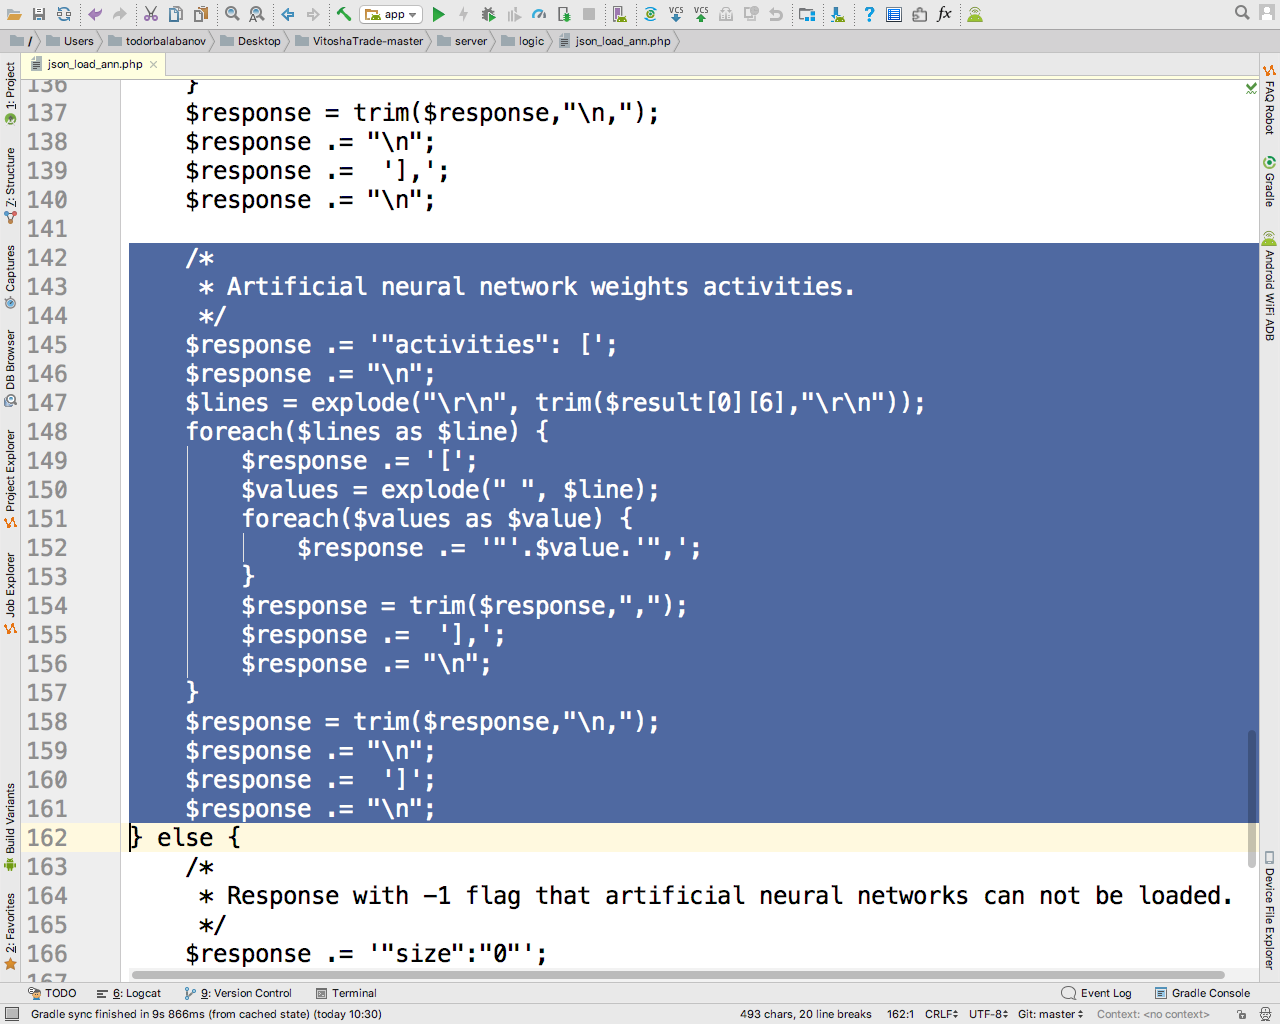
\includegraphics[height=0.45\pdfpageheight]{pic0120}
  \caption{Информация за теглата}
\label{fig:pic0120}
\end{figure}
\FloatBarrier

В ситуацията, когато екземплярът не е открит се връща нулев флаг. И при двата случая (открит или не) JSON съобщението се завършва, базата данни се затваря и информацията се изпраща към клиента (Фиг. \ref{fig:pic0121}).

\begin{figure}[h]
  \centering
  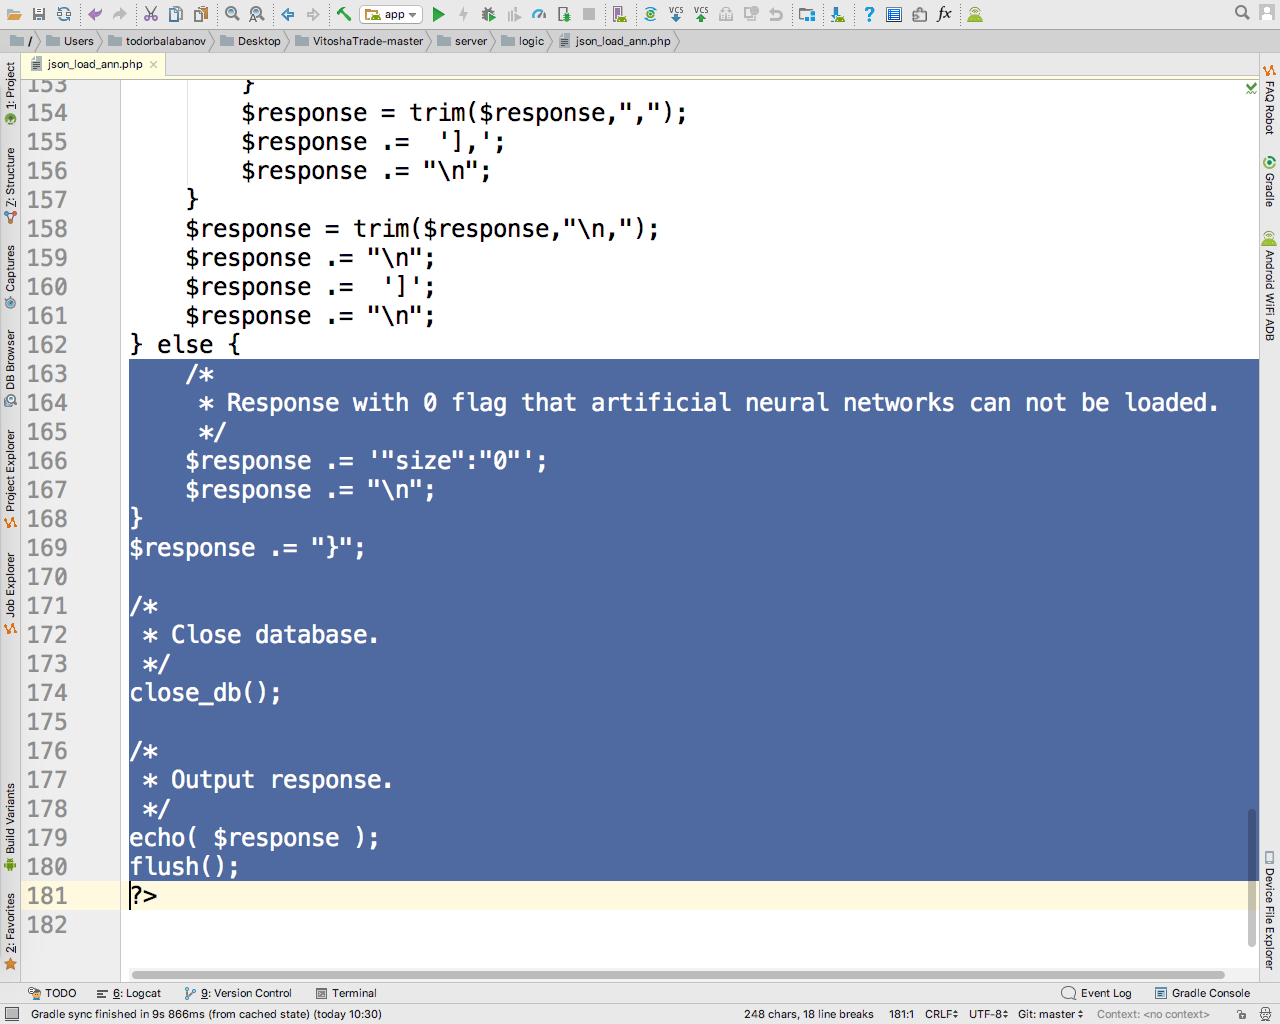
\includegraphics[height=0.45\pdfpageheight]{pic0121}
  \caption{Приключване на процедурата по изпращане на отговор}
\label{fig:pic0121}
\end{figure}
\FloatBarrier

\subsection{Зареждане на случайно избрана мрежа}

Когато изчисленията се извършват на принципа за дарената изчислителна мощност, логично е изборът на мрежата, която ще бъде допълнително тренирана  да е на случаен принцип. За тази цел, скриптът от страна на сървъра избира мрежата по случаен начин.

\begin{figure}[h]
  \centering
  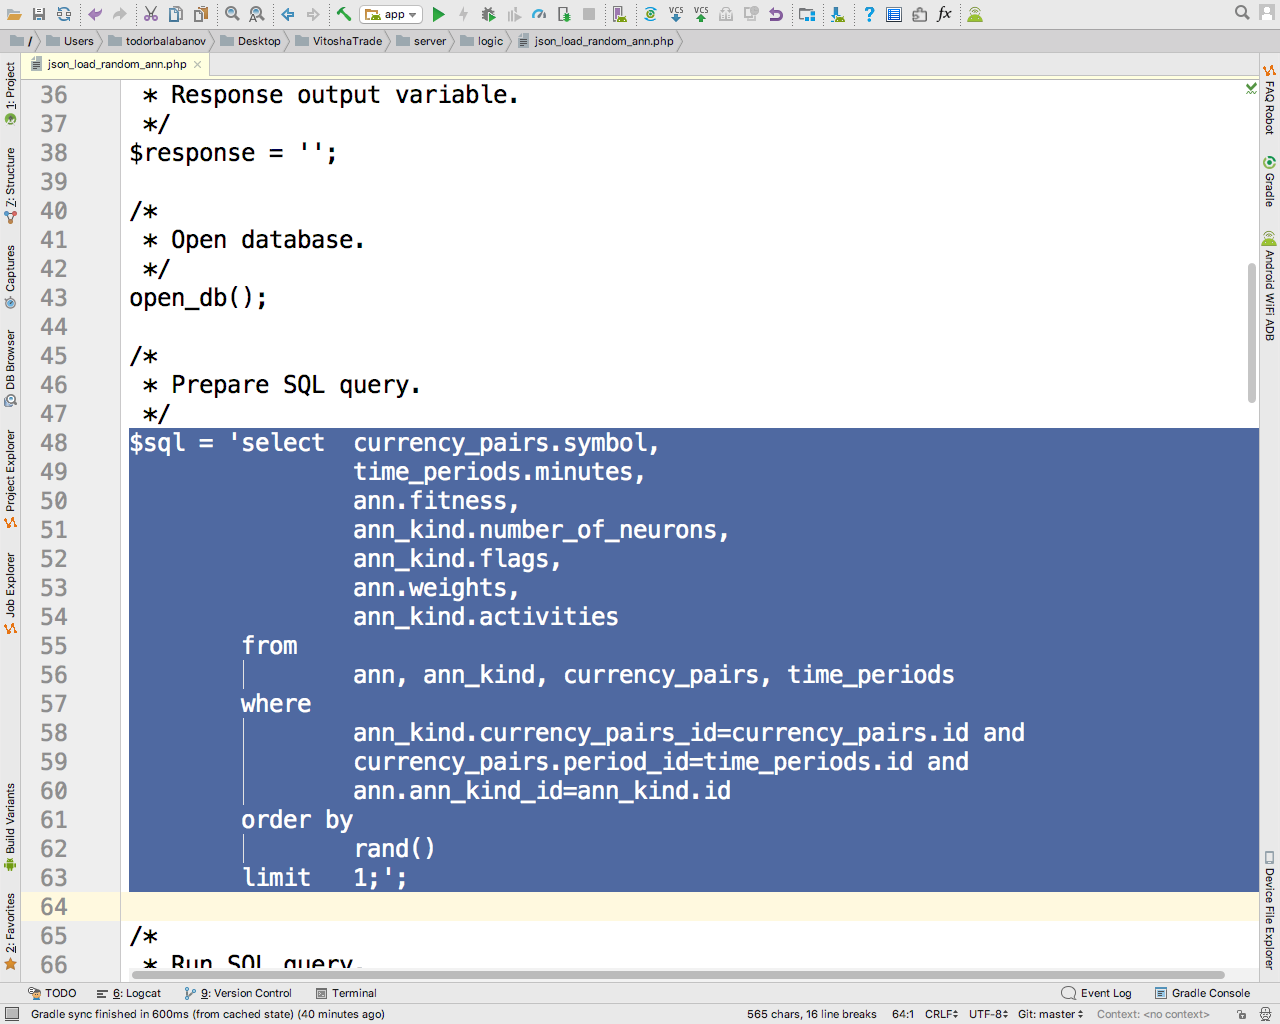
\includegraphics[height=0.45\pdfpageheight]{pic0157}
  \caption{Заявка за зареждане на случайна мрежа}
\label{fig:pic0157}
\end{figure}
\FloatBarrier

Единствената разлика от зареждането на мрежа по идентификатори и случайно избрана мрежа е в SQL заявката, която се изпълнява от MySQL (Фиг. \ref{fig:pic0157}).

\subsection{Зареждане на най-добрата жизненост от глобалната популация}

Един от основните критерии, по които клиентските приложения вземат решение дали да докладват откритите от тях резултати, е стойността на най-добрата жизненост в глобалната популация (популацията, която се съхранява на сървъра). Скриптът, отговарящ за тази проверка, също включва модула за работа с базата данни и извършва серия проверки на входните параметри. 

\begin{figure}[h]
  \centering
  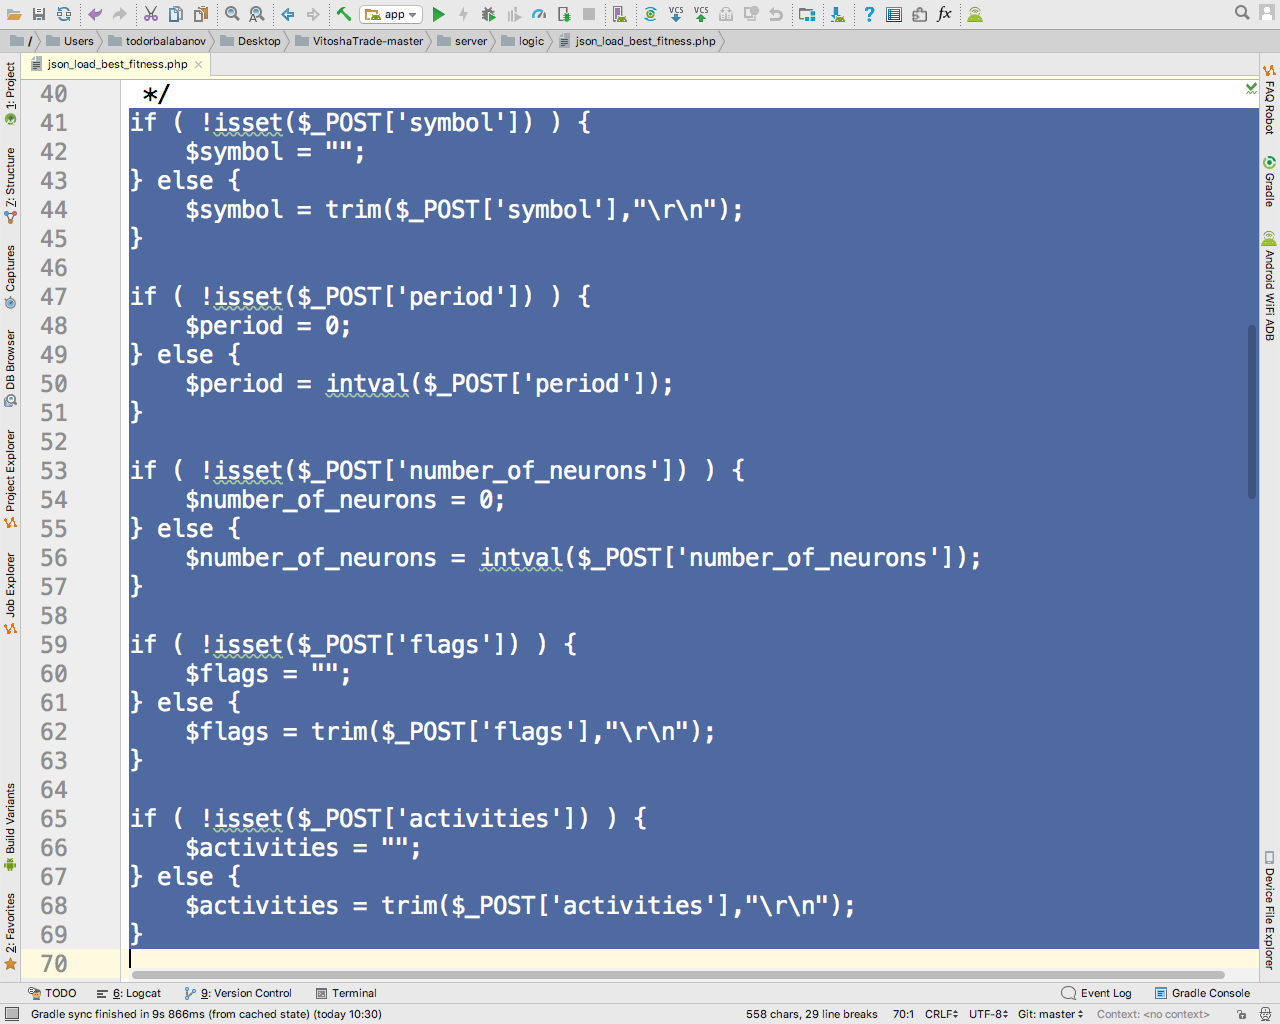
\includegraphics[height=0.45\pdfpageheight]{pic0122}
  \caption{Входни параметри за конкретна топология на невронна мрежа}
\label{fig:pic0122}
\end{figure}
\FloatBarrier

Проверяват се названието на валутната двойка, периодът на времевия ред, броят и типовете на невроните, както и връзките между тях (Фиг. \ref{fig:pic0122}).

\begin{figure}[h]
  \centering
  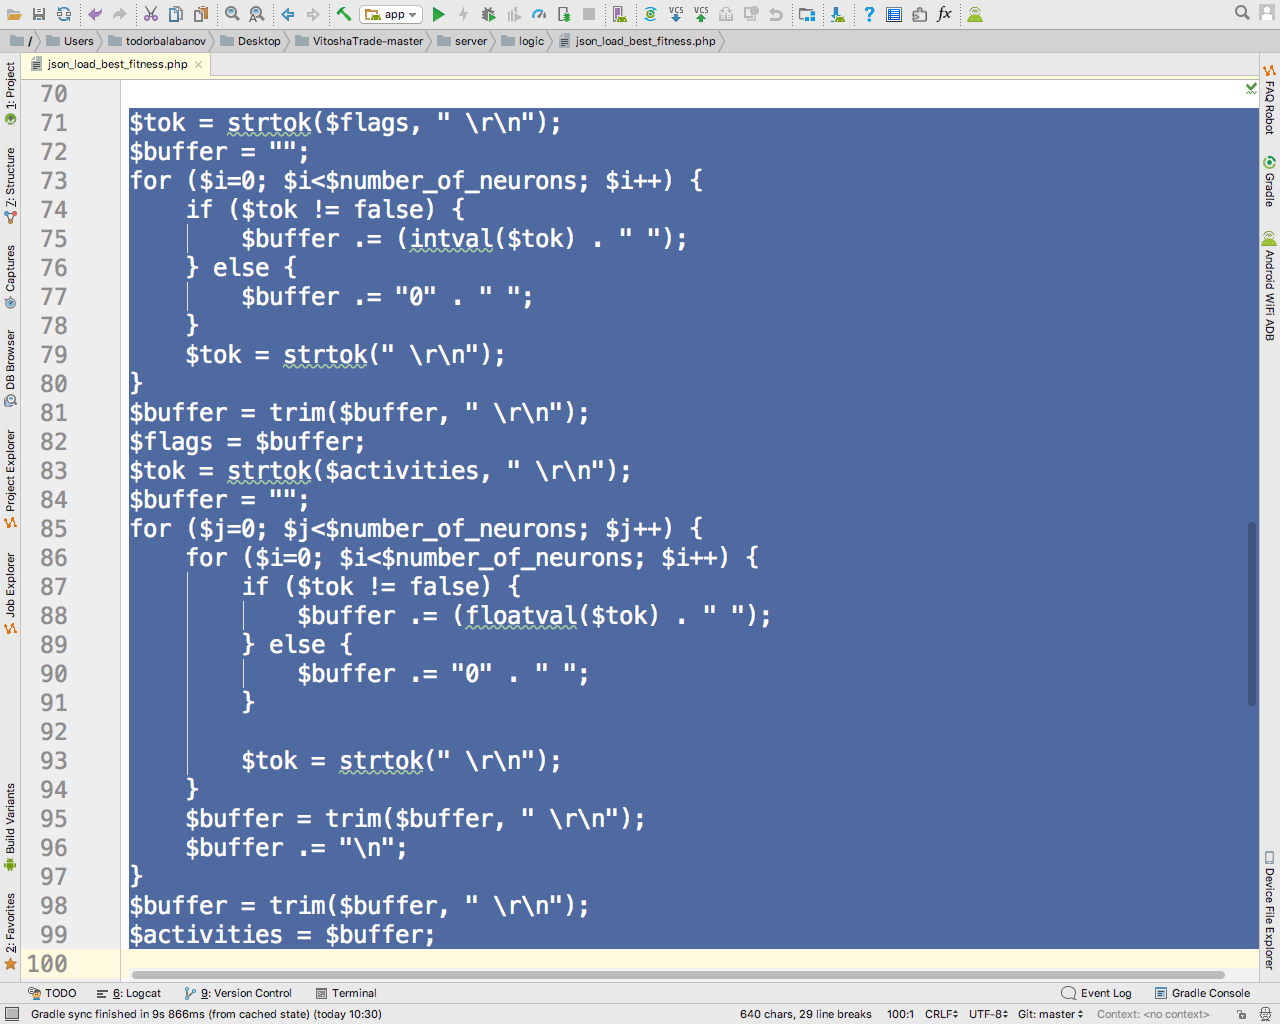
\includegraphics[height=0.45\pdfpageheight]{pic0123}
  \caption{Флагове на невроните и връзките между тях}
\label{fig:pic0123}
\end{figure}
\FloatBarrier

Тъй като типовете на невроните са представени като масив, а връзките между самите неврони в матрица на съседство, то проверката им изисква малко по-сложна обработка в цикли (Фиг. \ref{fig:pic0123}).

\begin{figure}[h]
  \centering
  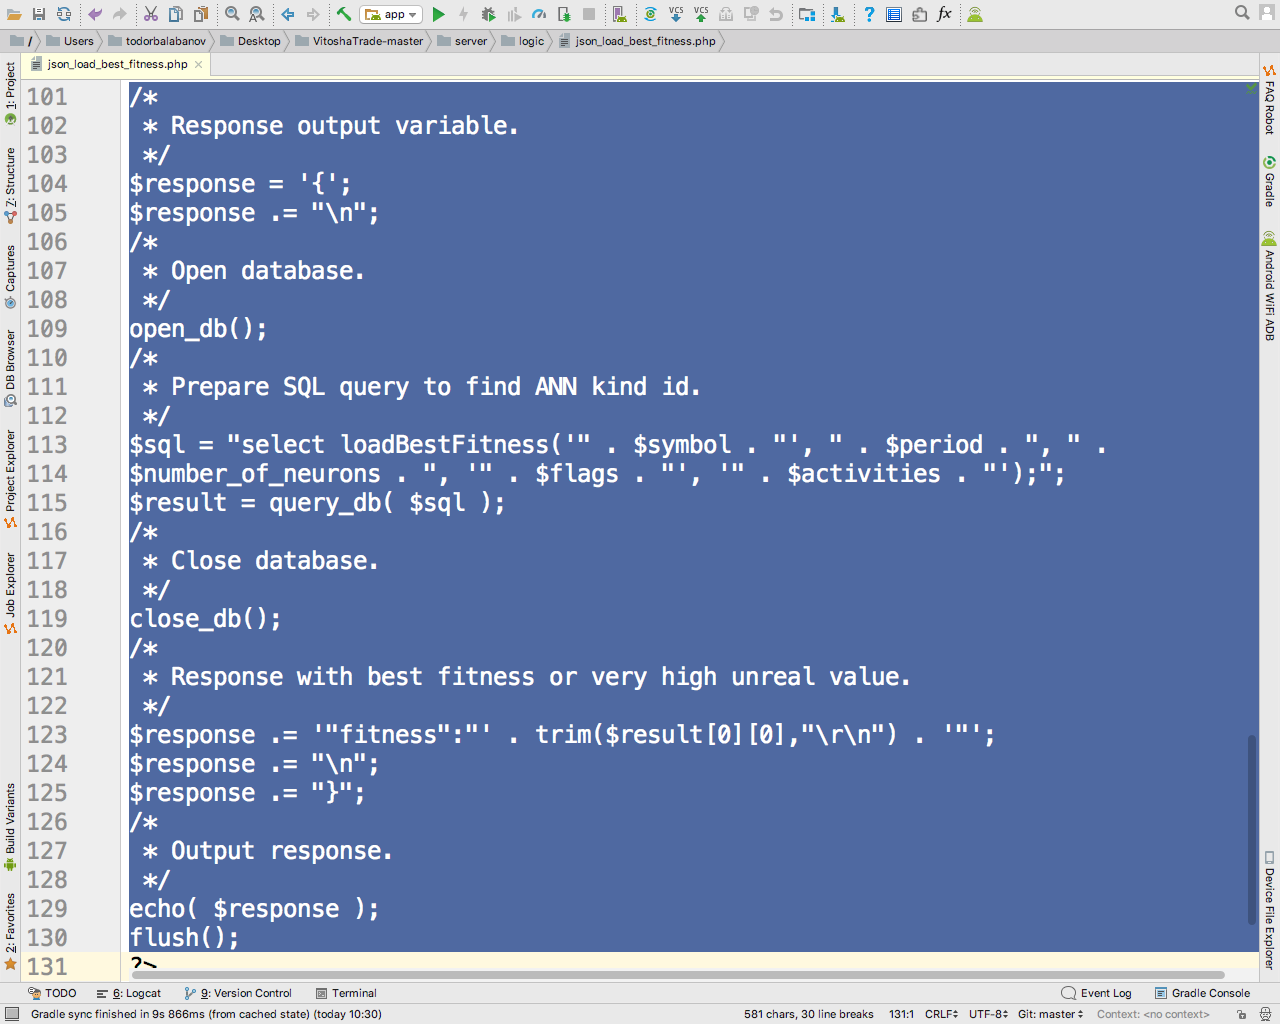
\includegraphics[height=0.45\pdfpageheight]{pic0124}
  \caption{Заявка за най-добра жизненост}
\label{fig:pic0124}
\end{figure}
\FloatBarrier

Следва отваряне на връзката към базата данни, изпълнение на съхранената функция за откриване на най-добра жизненост, затваряне на базата данни и изпращане до клиента на JSON пакетиран отговор (Фиг. \ref{fig:pic0124}).

\subsection{Зареждане на брой неврони по идентификатор}

При работата с екземпляри на изкуствените невронни мрежи, съществено е запитването за броя неврони в мрежата. 

\begin{figure}[h]
  \centering
  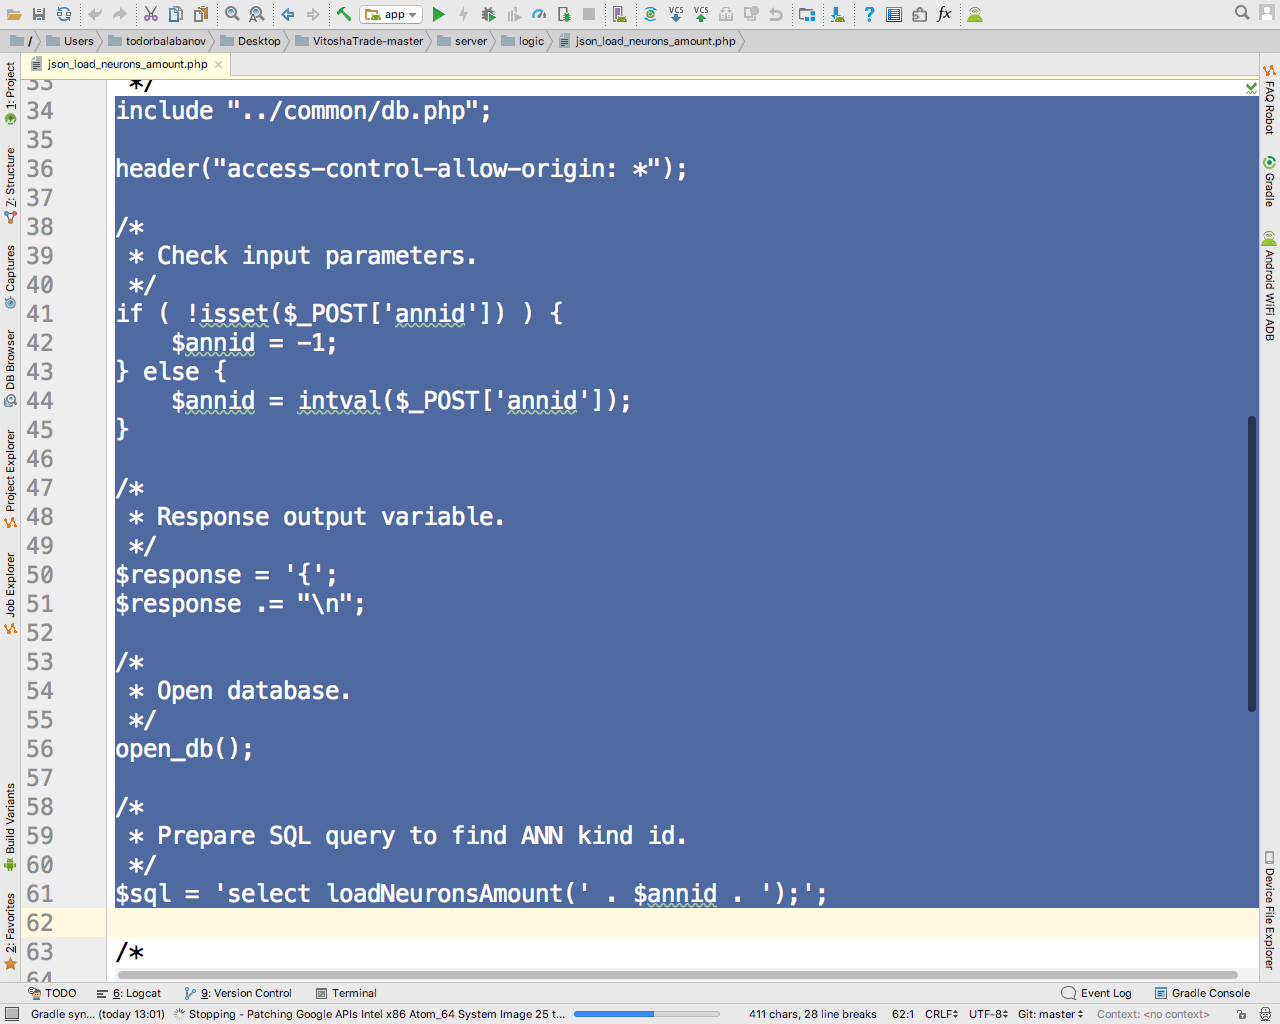
\includegraphics[height=0.45\pdfpageheight]{pic0125}
  \caption{Определяне на броя неврони по идентификатор на мрежа}
\label{fig:pic0125}
\end{figure}
\FloatBarrier

Процедурата отново включва модула за работа с базата данни, проверка на входния параметър за идентификатор на екземпляр, отваряне на връзка към базата данни и стартиране на съхранена функция (Фиг. \ref{fig:pic0125}).

\begin{figure}[h]
  \centering
  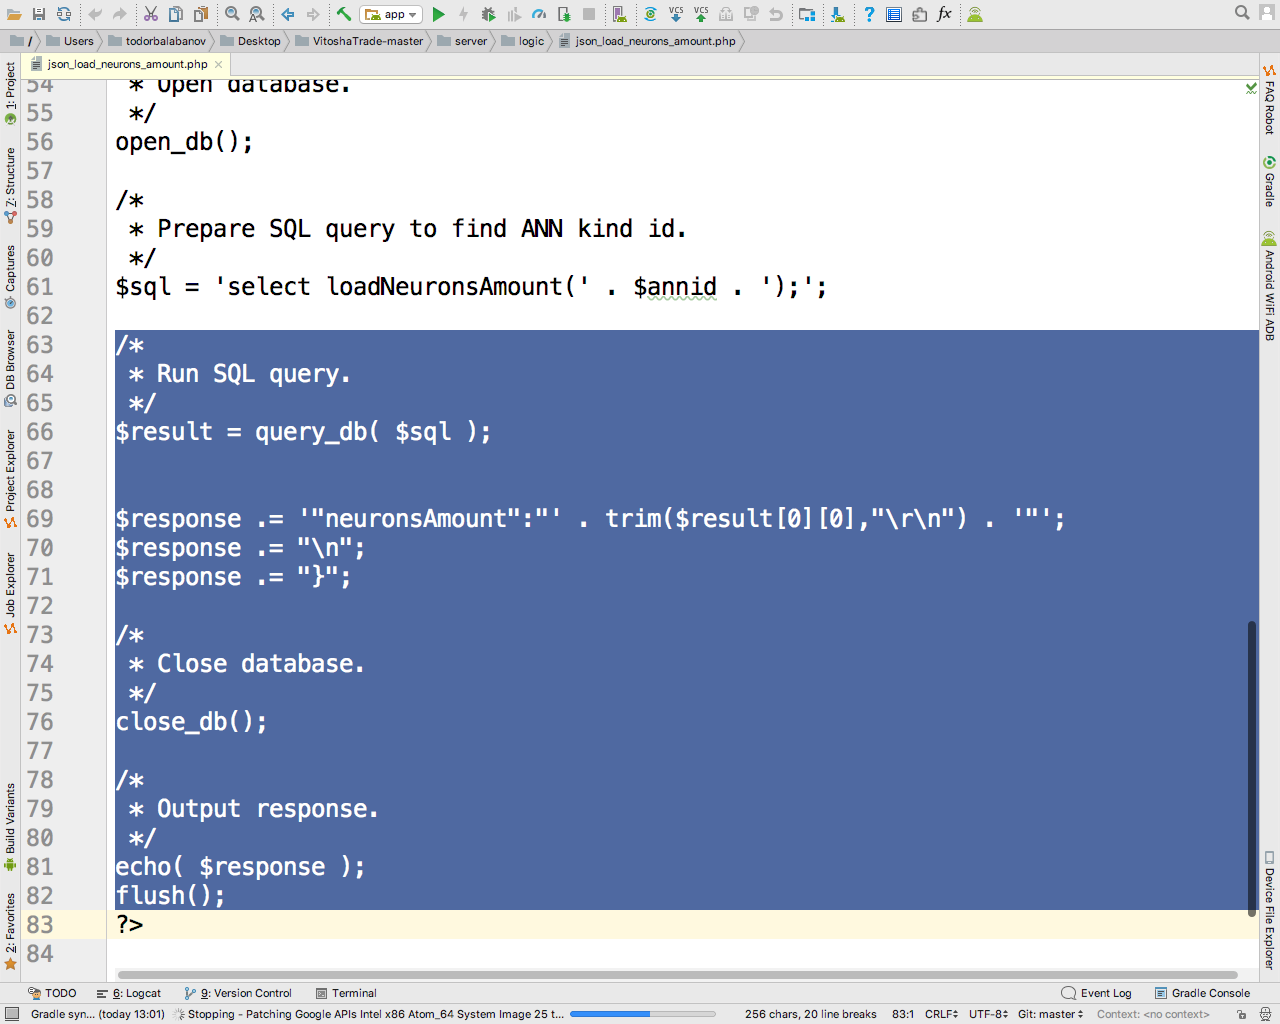
\includegraphics[height=0.45\pdfpageheight]{pic0126}
  \caption{Отговор към клиента}
\label{fig:pic0126}
\end{figure}
\FloatBarrier

Резултатът от съхранената функция се опакова в JSON съобщение и се изпраща на клиента (Фиг. \ref{fig:pic0126}).

\subsection{Зареждане на тренировъчно множество по информация за валутна двойка}

За обучението на всяка изкуствена невронна мрежа се използва тренировъчно множество, което е различно, според названието на валутната двойка и времевия интервал на реда. 

\begin{figure}[h]
  \centering
  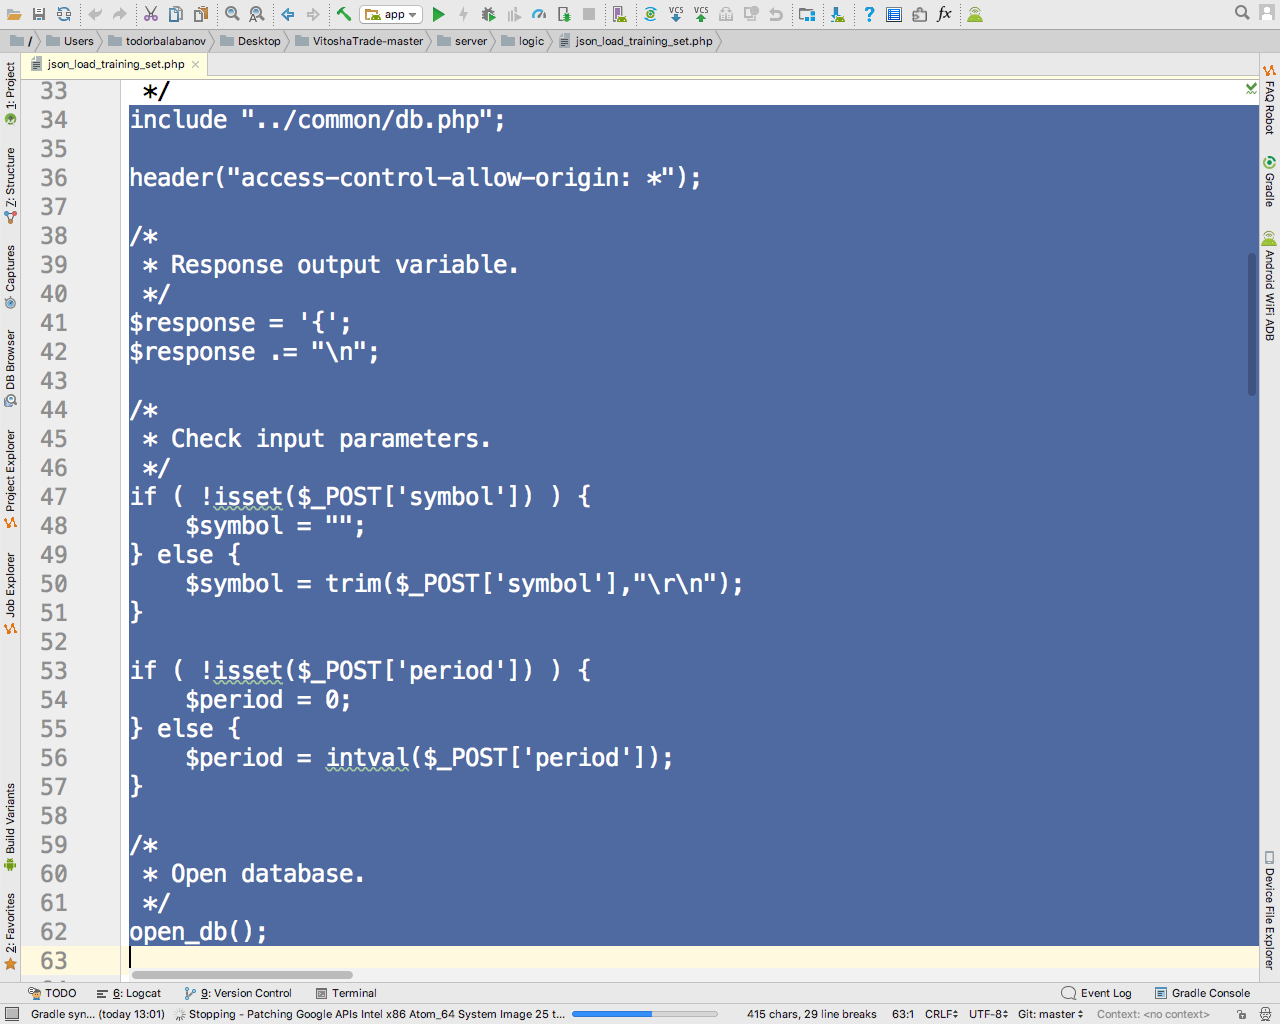
\includegraphics[height=0.45\pdfpageheight]{pic0127}
  \caption{Проверка на входните параметри}
\label{fig:pic0127}
\end{figure}
\FloatBarrier

Зареждането започва по класическия начин с включване на модула за работа с базата данни, проверка на входната информация и отваряне на връзка към базата данни (Фиг. \ref{fig:pic0127}).

\begin{figure}[h]
  \centering
  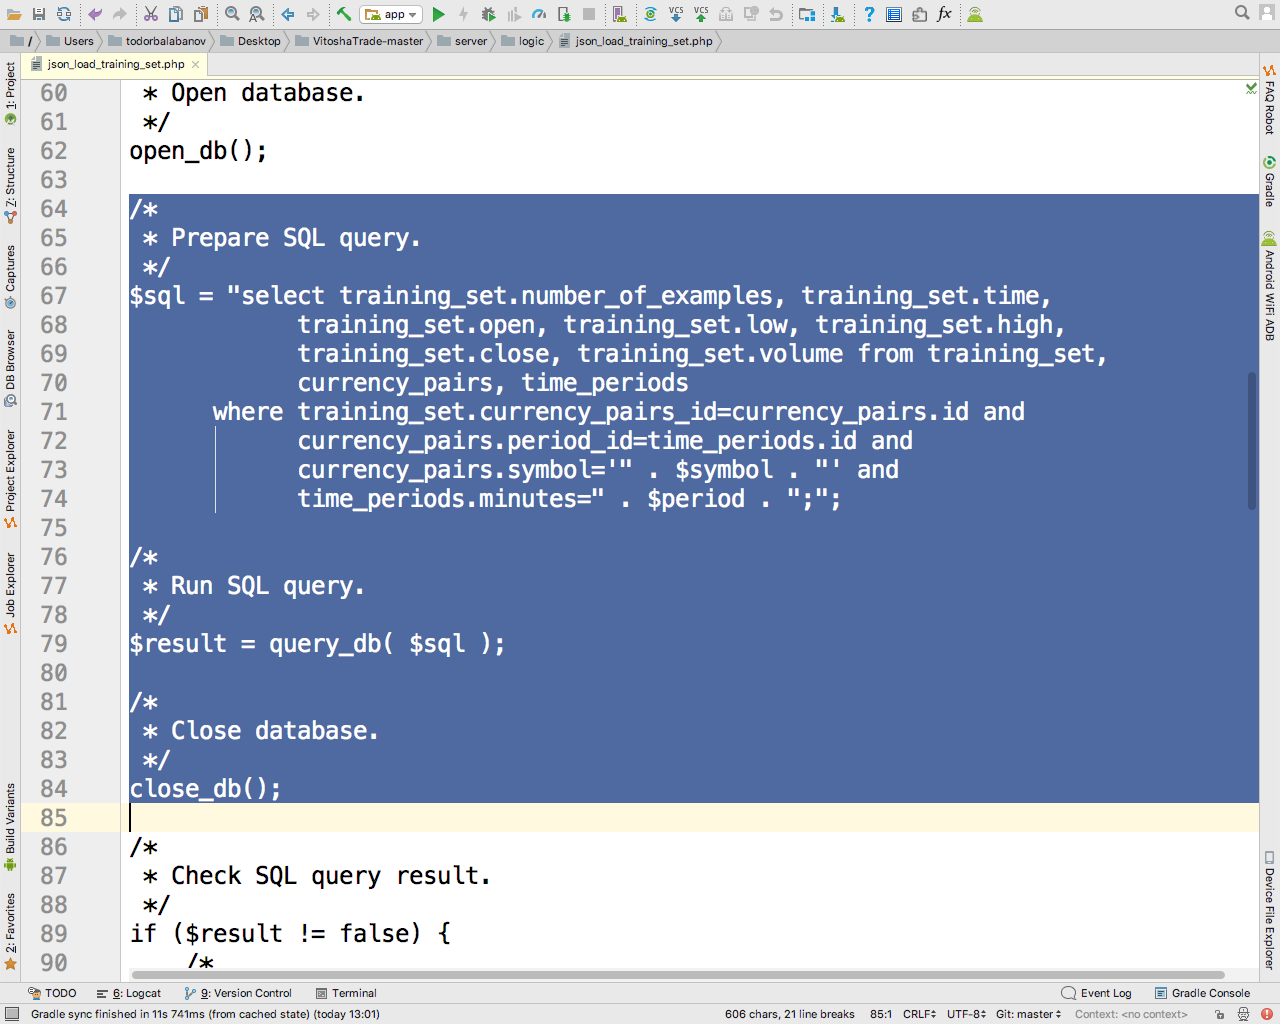
\includegraphics[height=0.45\pdfpageheight]{pic0128}
  \caption{Заявка за тренировъчно множество}
\label{fig:pic0128}
\end{figure}
\FloatBarrier

Следва заявка, извличане на резултата и затваряне на връзката към базата данни (Фиг. \ref{fig:pic0128}). Макар и да не е направено, добрият стил за разделяне на слоевете предполага вместо заявка да се извика съхранена функция. 

\begin{figure}[h]
  \centering
  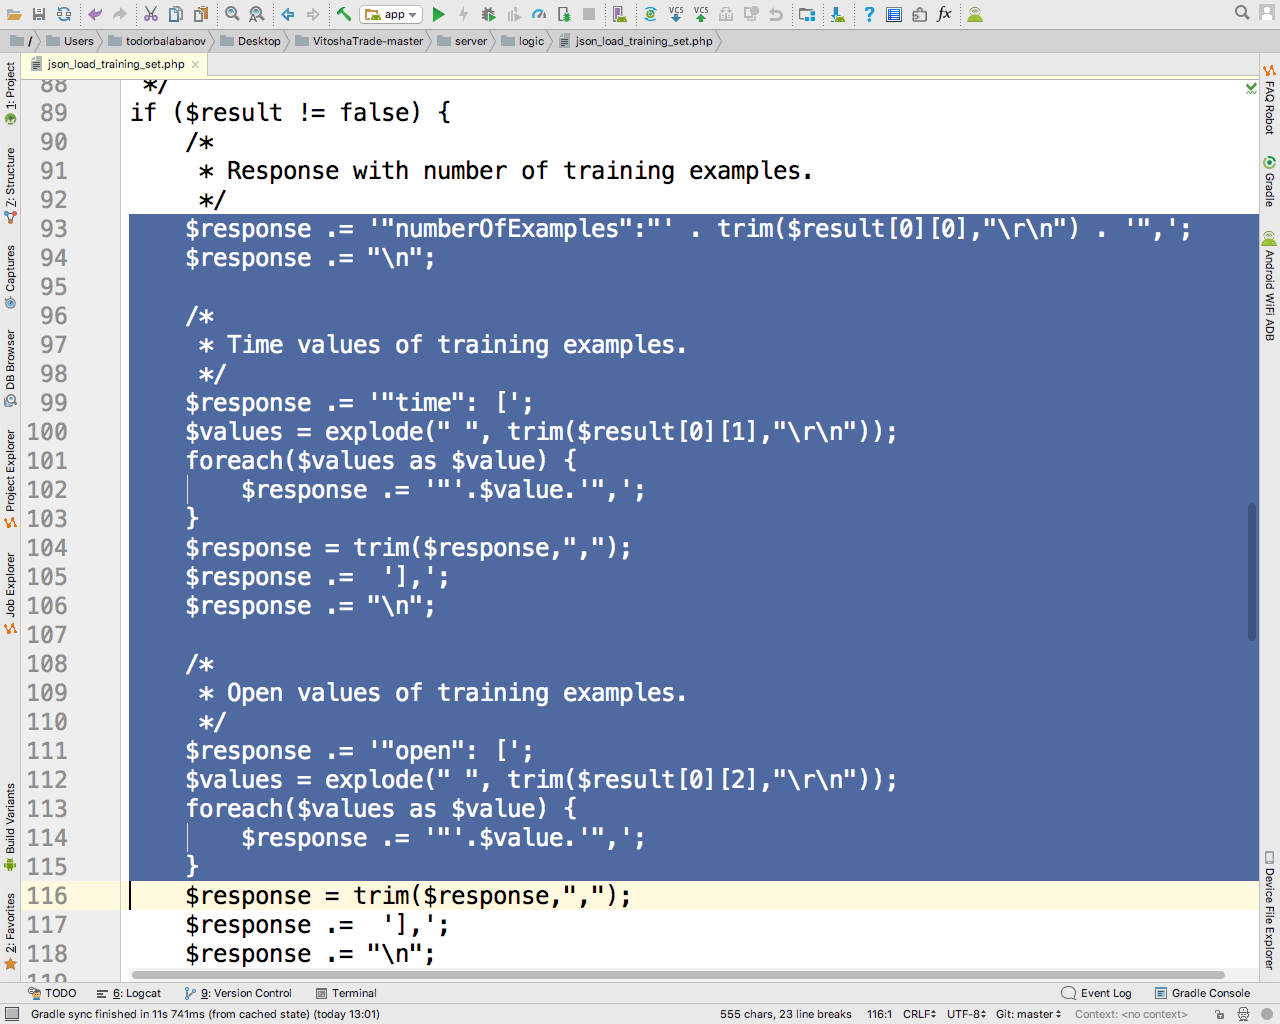
\includegraphics[height=0.45\pdfpageheight]{pic0129}
  \caption{Брой примери, времеви маркери и нива на отваряне}
\label{fig:pic0129}
\end{figure}
\FloatBarrier

\begin{figure}[h]
  \centering
  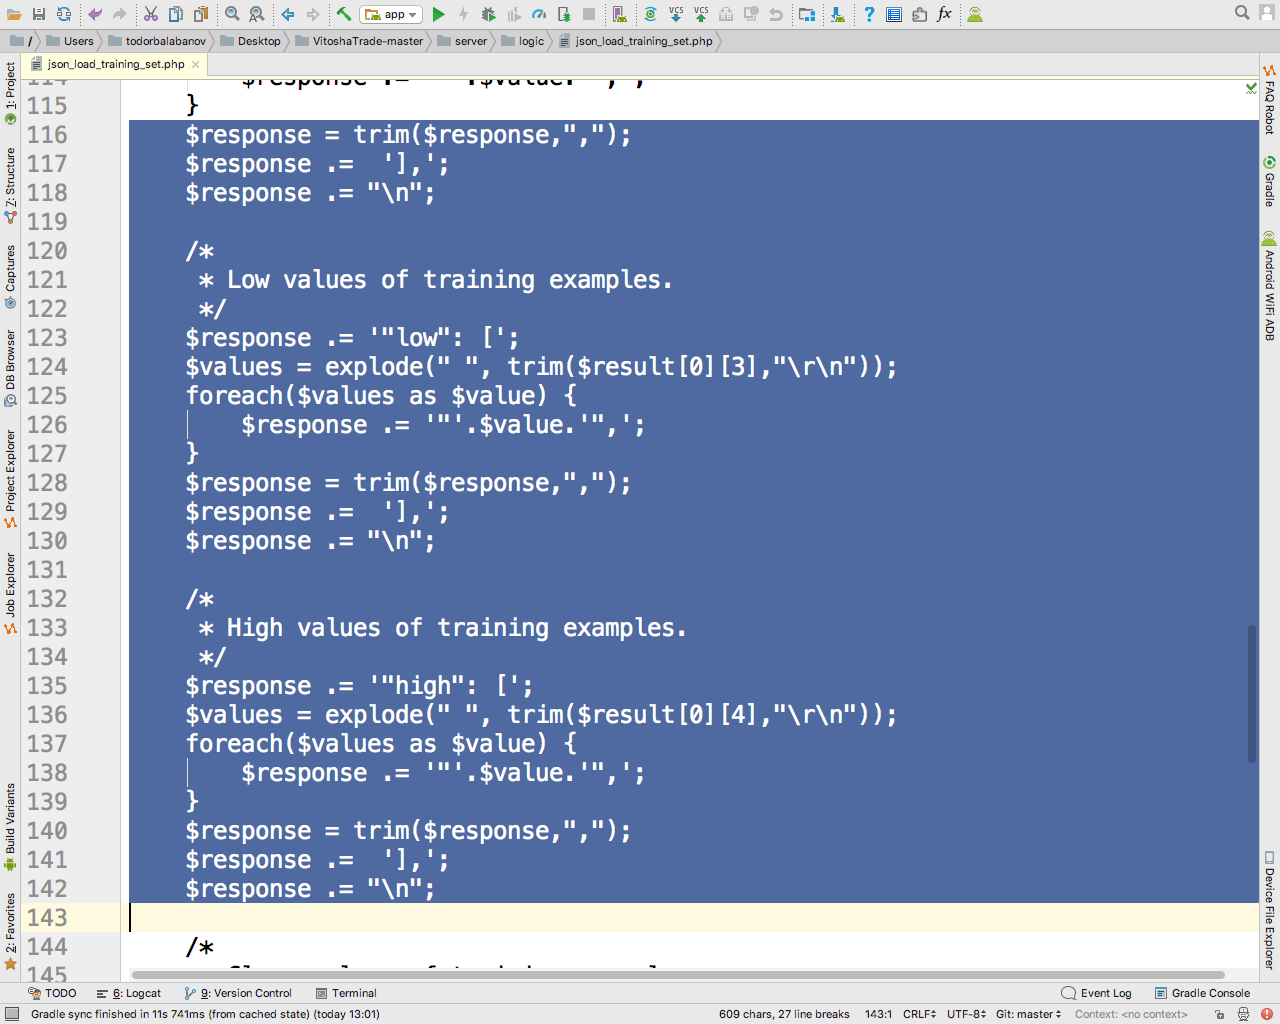
\includegraphics[height=0.45\pdfpageheight]{pic0130}
  \caption{Най-ниска и най-висока постигната стойност}
\label{fig:pic0130}
\end{figure}
\FloatBarrier

\begin{figure}[h]
  \centering
  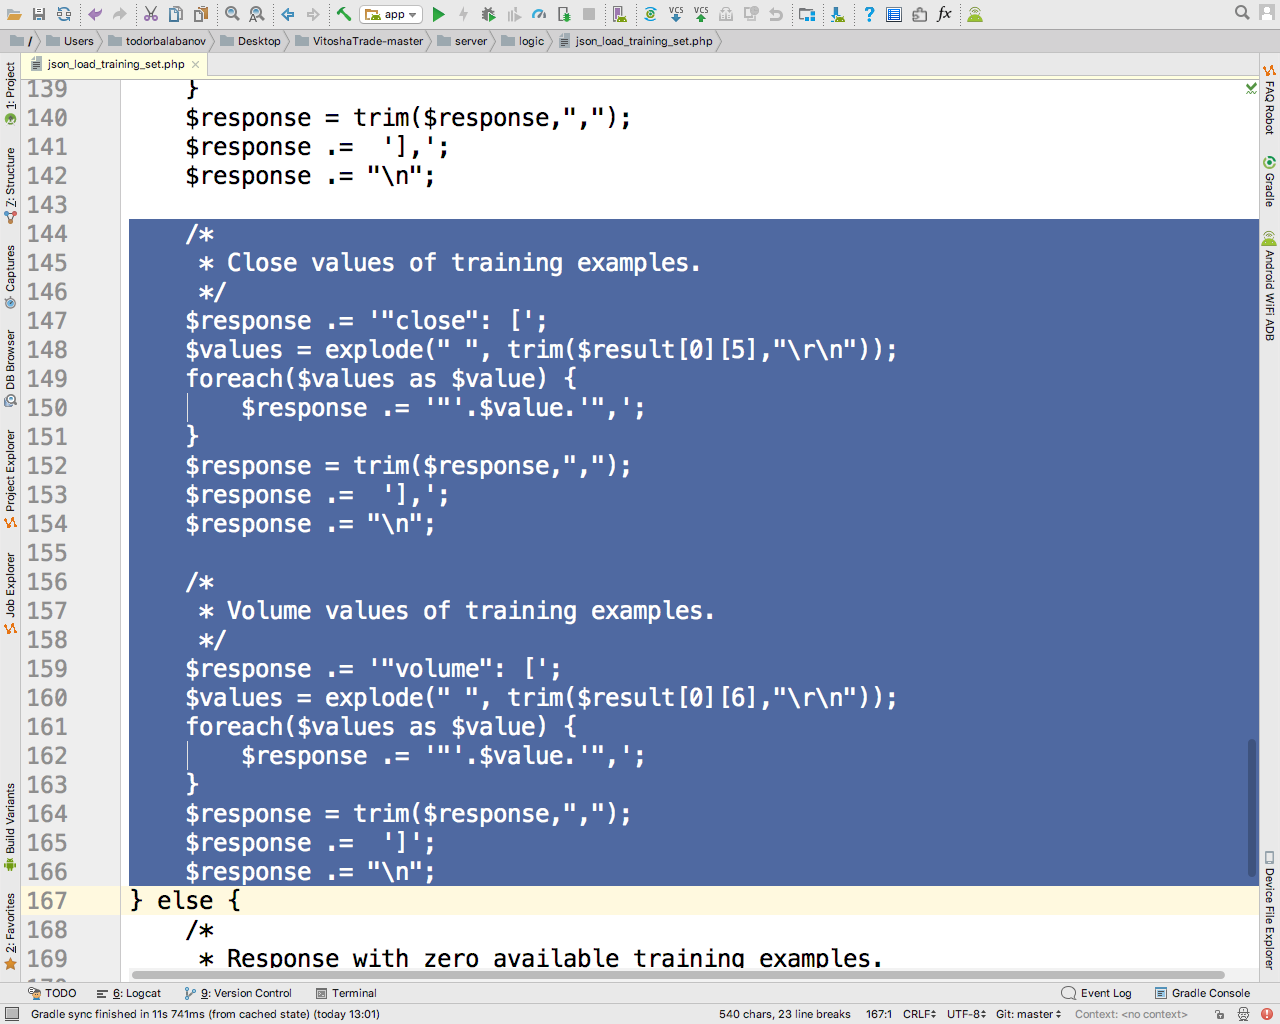
\includegraphics[height=0.45\pdfpageheight]{pic0131}
  \caption{Нива на затваряне и търгуван обем}
\label{fig:pic0131}
\end{figure}
\FloatBarrier

Ако е намерено тренировъчно множество за посочената валутна двойка и времеви интервал, то стойностите от времевия ред се пакетират и изпращат на клиента (Фиг. \ref{fig:pic0129}-\ref{fig:pic0131}).

\begin{figure}[h]
  \centering
  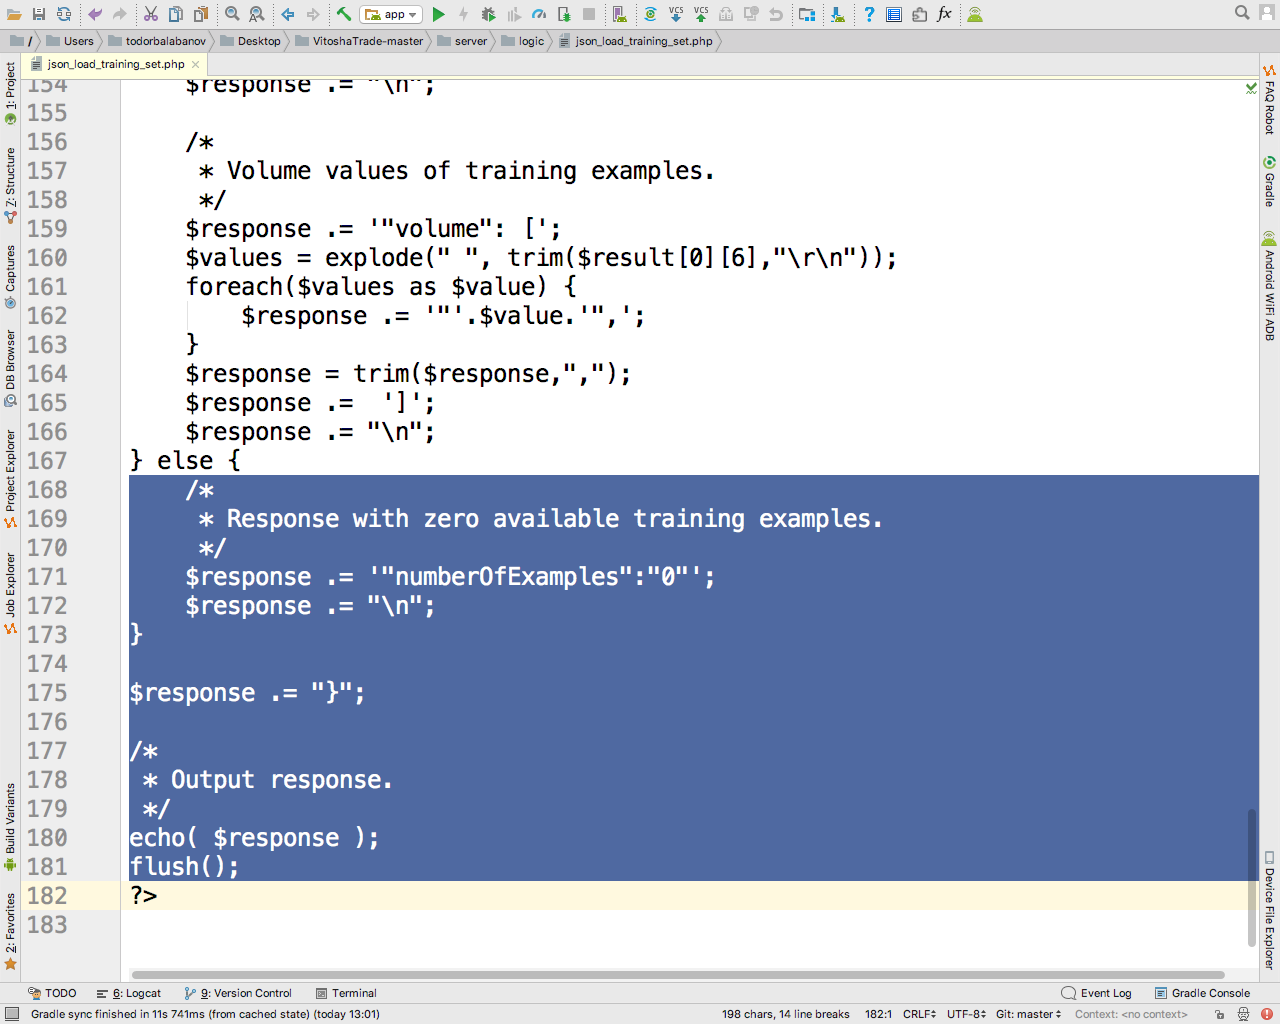
\includegraphics[height=0.45\pdfpageheight]{pic0132}
  \caption{Изпращане на отговор до клиента}
\label{fig:pic0132}
\end{figure}
\FloatBarrier

Ако тренировъчно множество не бъде открито, се изпраща съобщение с нулев размер за данните. Без значение дали е открито множество или не, JSON съобщението се изпраща до клиента (Фиг. \ref{fig:pic0132}).

\subsection{Зареждане на брой екземпляри по идентификатор или информация за валутна двойка}

За подбирането на подмножество от глобалната популация е нужно да се знае колко екземпляра присъстват в базата данни по зададен идентификатор на екземпляр или название на валутна двойка с период. 

\begin{figure}[h]
  \centering
  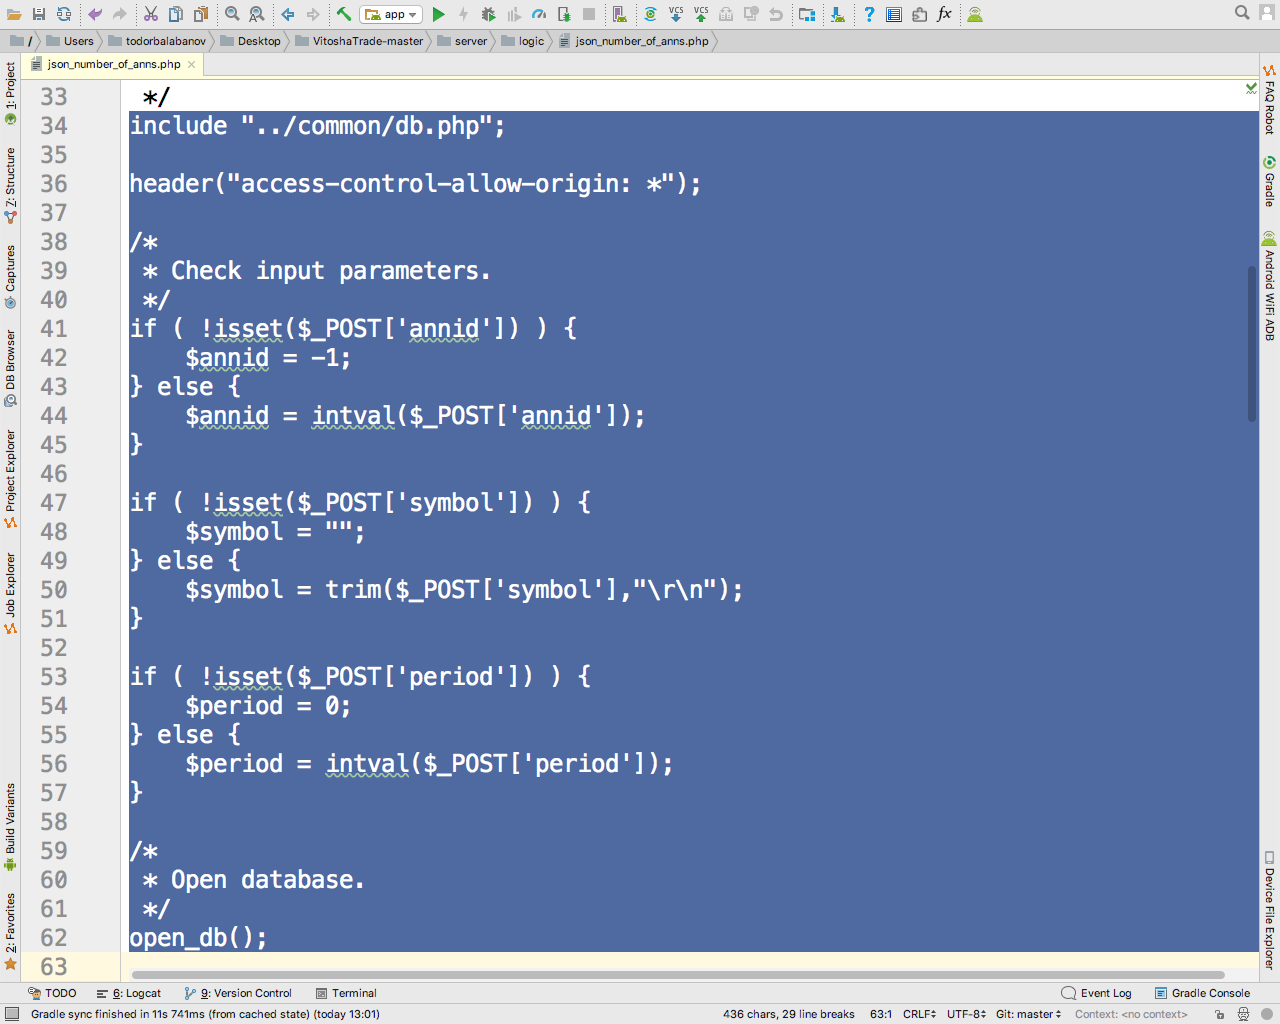
\includegraphics[height=0.45\pdfpageheight]{pic0133}
  \caption{Проверка на входните аргументи}
\label{fig:pic0133}
\end{figure}
\FloatBarrier

Проверката отново започва с включване на модула за работа с базата данни, проверка на входните аргументи и отваряне на връзка към базата данни (Фиг. \ref{fig:pic0133}).

\begin{figure}[h]
  \centering
  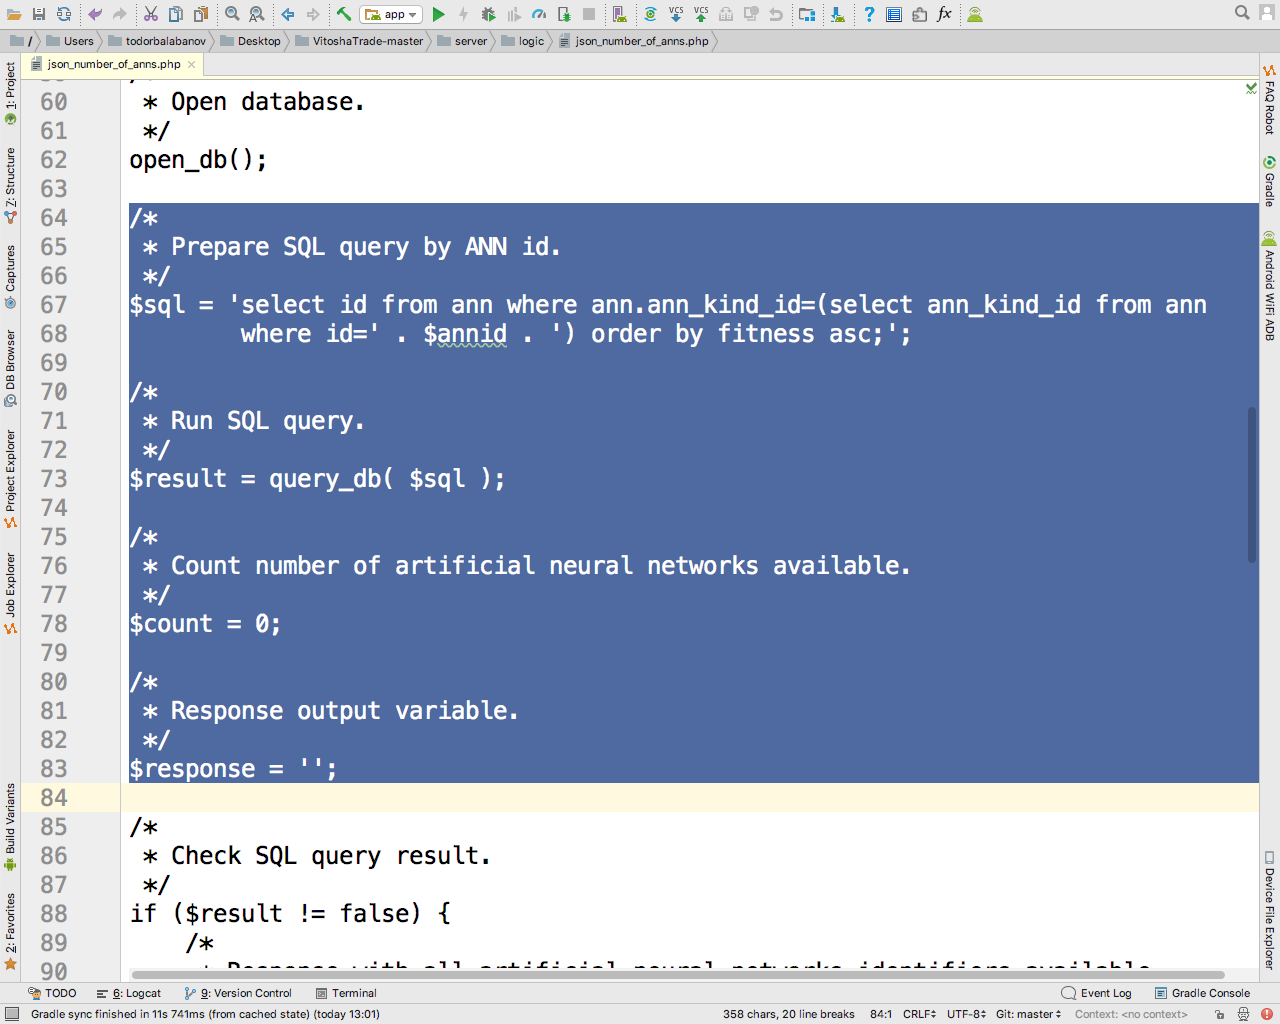
\includegraphics[height=0.45\pdfpageheight]{pic0134}
  \caption{Еземпляри от типа на подадения идентификатор}
\label{fig:pic0134}
\end{figure}
\FloatBarrier

Първо се изброяват екземплярит,е които са от типа на подадения идентификатор (Фиг. \ref{fig:pic0134}).

\begin{figure}[h]
  \centering
  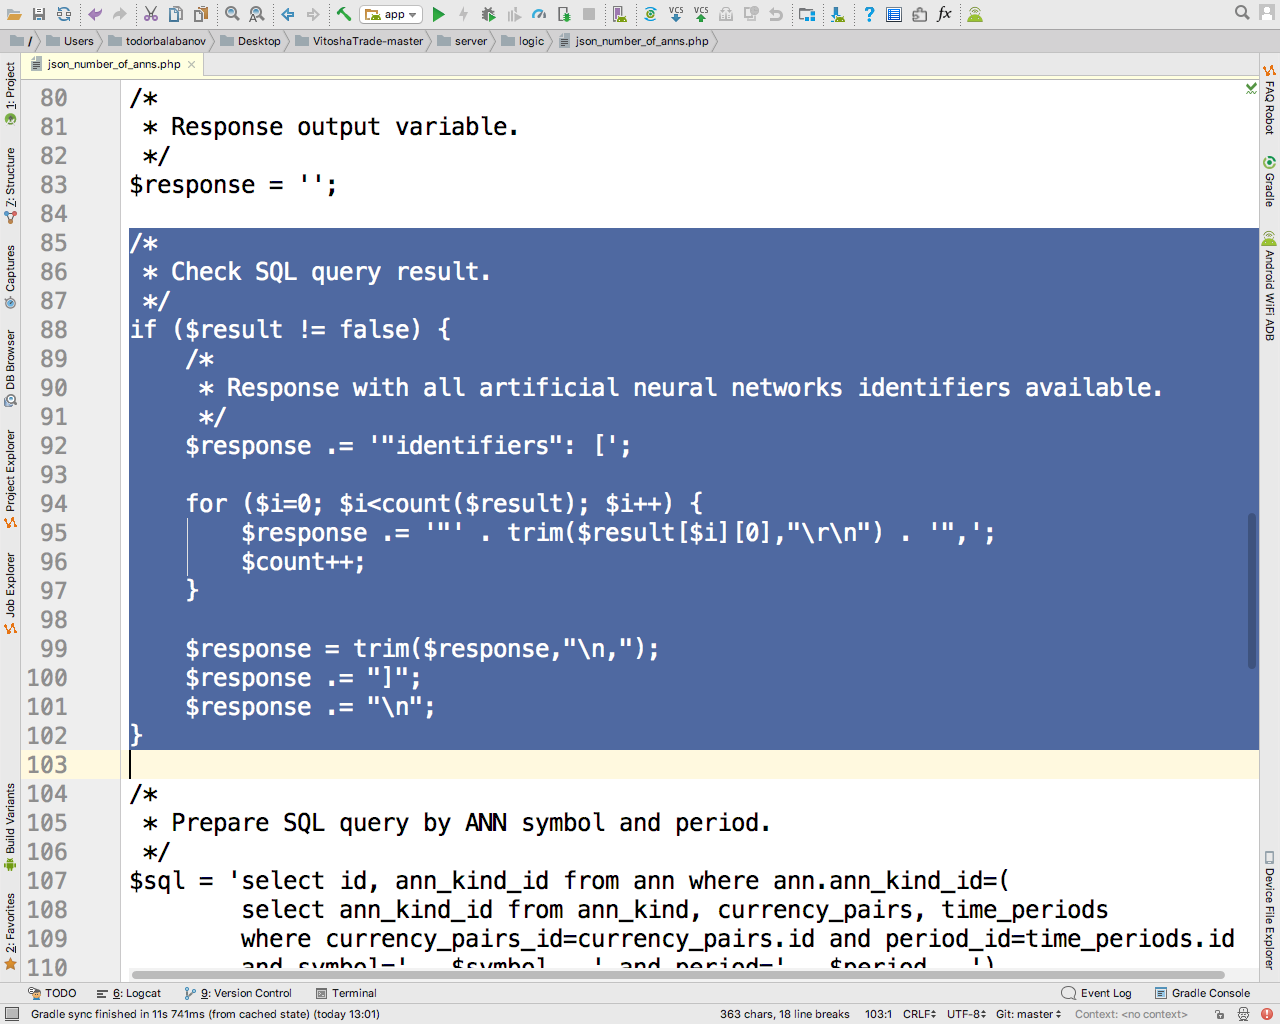
\includegraphics[height=0.45\pdfpageheight]{pic0135}
  \caption{Пакетиране на получените стойности в JSON съобщение}
\label{fig:pic0135}
\end{figure}
\FloatBarrier

Получените стойности се пакетират в JSON съобщение (Фиг. \ref{fig:pic0135}). 

\begin{figure}[h]
  \centering
  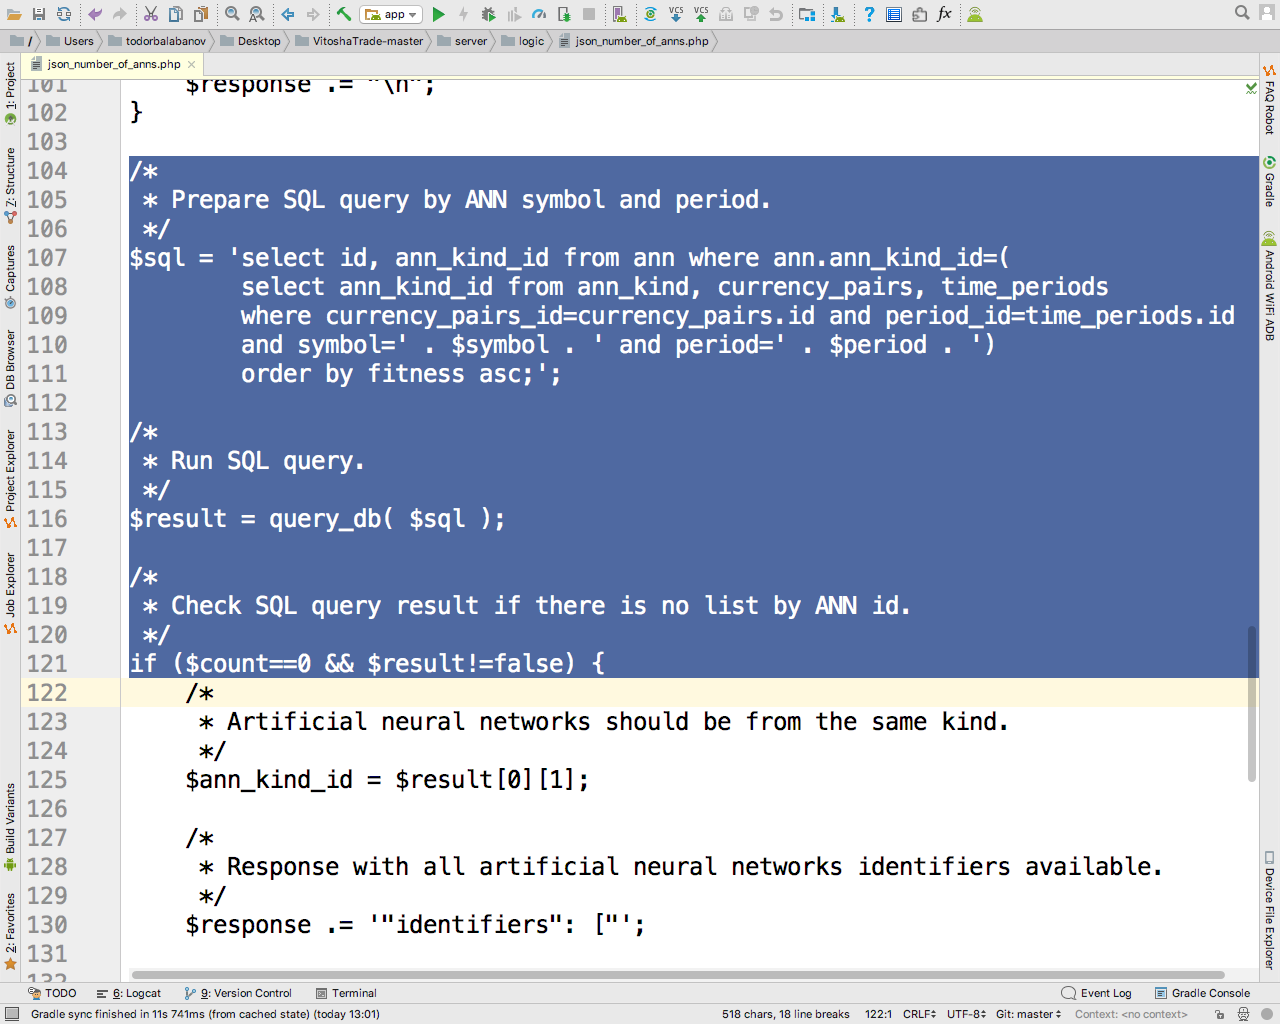
\includegraphics[height=0.45\pdfpageheight]{pic0136}
  \caption{Проверка за екземпляри по название на валутна двойка и период}
\label{fig:pic0136}
\end{figure}
\FloatBarrier

Следва проверка за екземпляри по название на валутна двойка и период. Този списък се използва само, ако първоначално не е открито подмножество (Фиг. \ref{fig:pic0136}).

\begin{figure}[h]
  \centering
  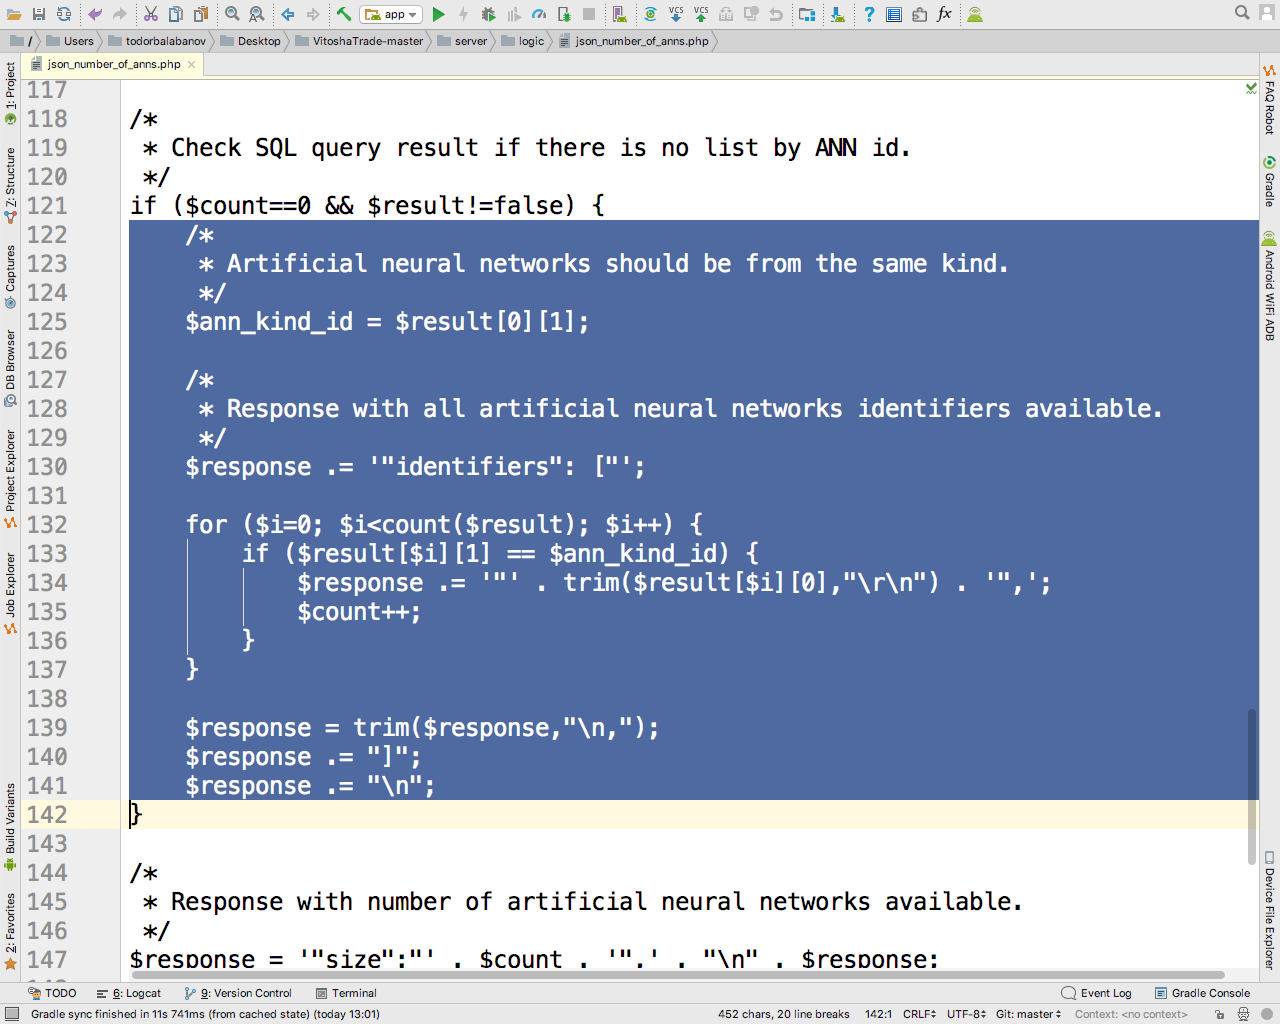
\includegraphics[height=0.45\pdfpageheight]{pic0137}
  \caption{Пакетиране на получените стойности в JSON съобщение}
\label{fig:pic0137}
\end{figure}
\FloatBarrier

Пакетирането в JSON съобщение е аналогично на предходното (Фиг. \ref{fig:pic0137}).

\begin{figure}[h]
  \centering
  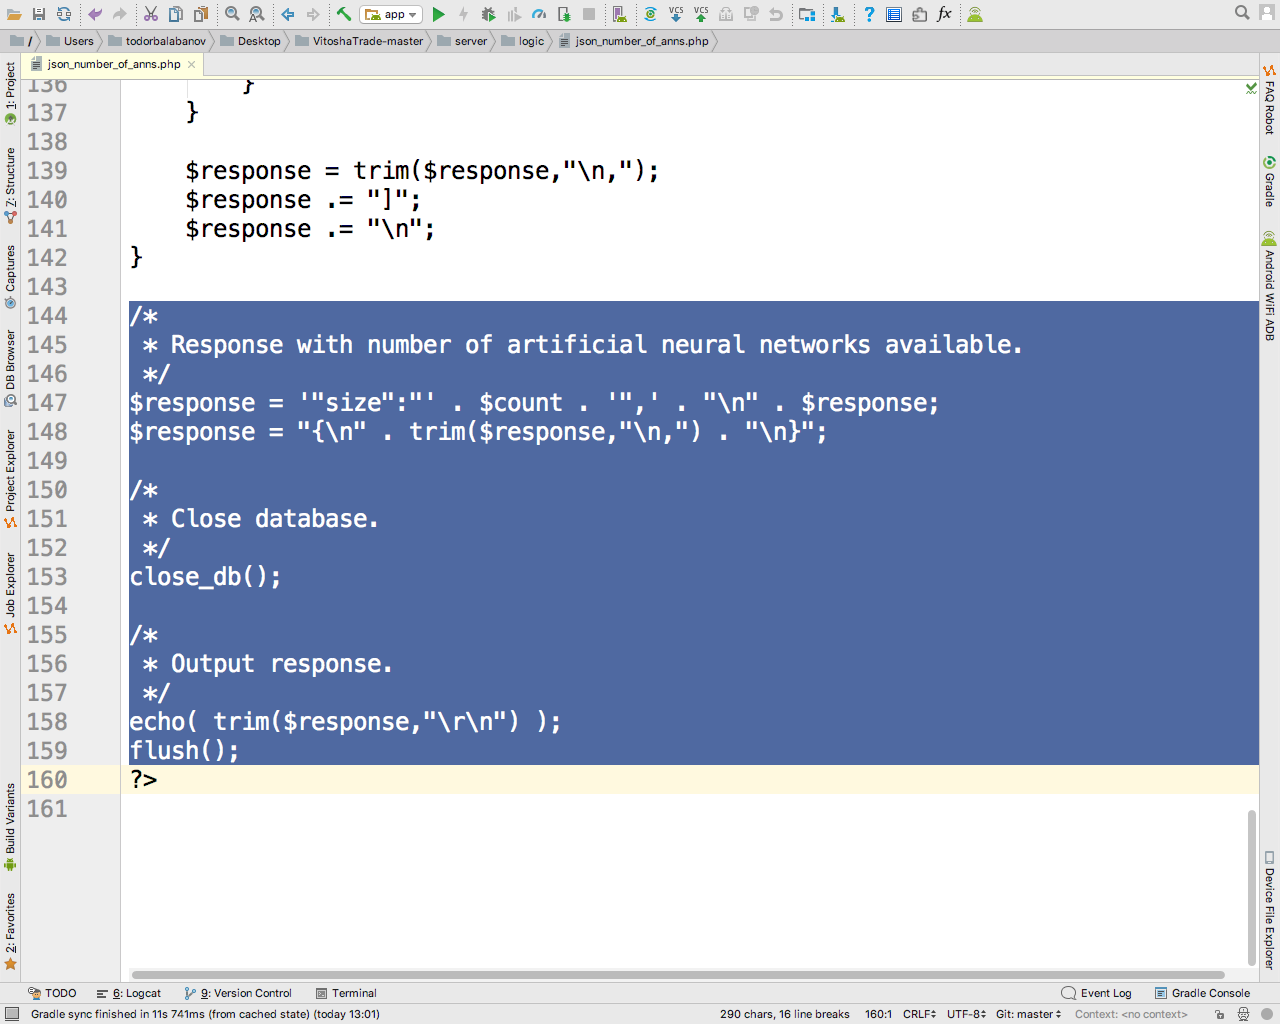
\includegraphics[height=0.45\pdfpageheight]{pic0138}
  \caption{Изпращане на резултата}
\label{fig:pic0138}
\end{figure}
\FloatBarrier

Скриптът завършва със затваряне на връзката към базата данни, оформяне и изпращане на резултата до клиента (Фиг. \ref{fig:pic0138}).

\subsection{Зареждане на брой тренировъчни примери по информация за валутна двойка}

За определянето на броя тренировъчни примери се подхожда по аналогичен начин с включване на модула за работа с базата данни, проверка на входните аргументи и отваряне на връзка към базата данни (Фиг. \ref{fig:pic0139}). 

\begin{figure}[h]
  \centering
  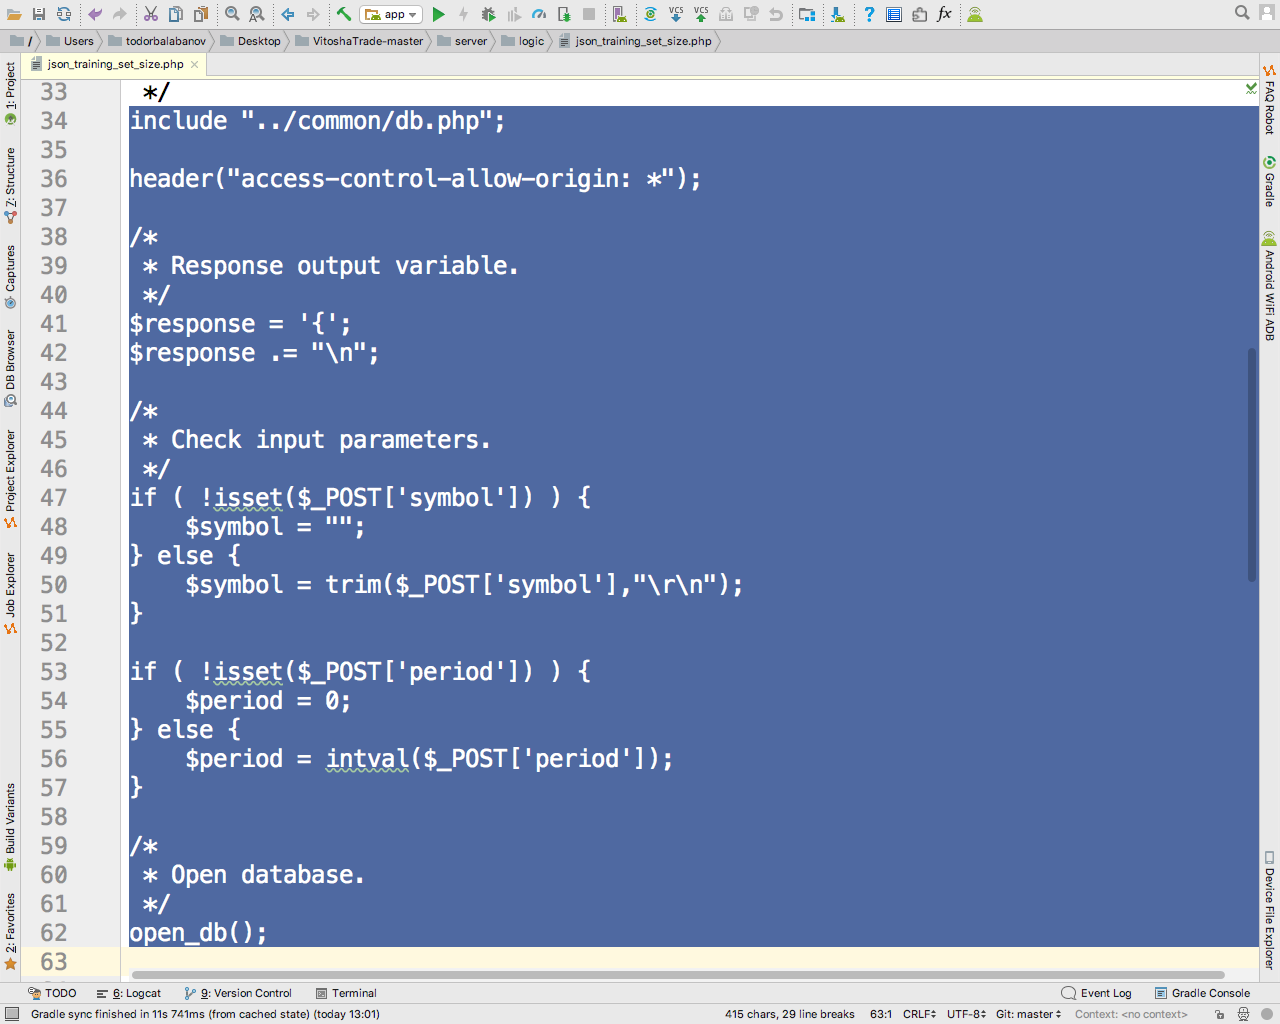
\includegraphics[height=0.45\pdfpageheight]{pic0139}
  \caption{Брой тренировъчни примери по валутна информация}
\label{fig:pic0139}
\end{figure}
\FloatBarrier

Изпълнението на заявката може да открие подходящо тренировъчно множество или да не открие такова (Фиг. \ref{fig:pic0140}). 

\begin{figure}[h]
  \centering
  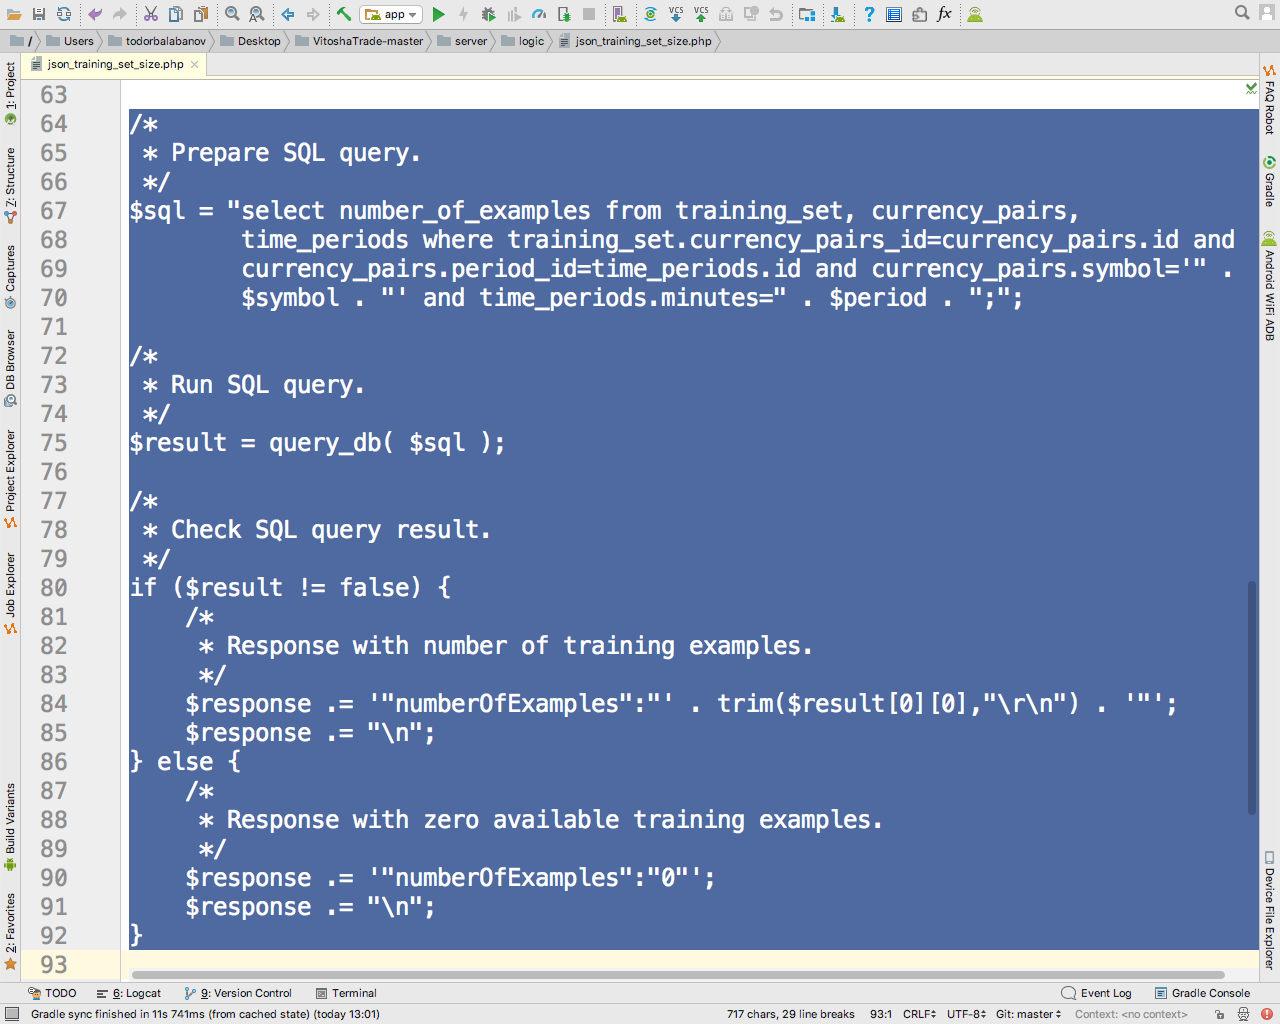
\includegraphics[height=0.45\pdfpageheight]{pic0140}
  \caption{Заявка за брой тренировъчни примери}
\label{fig:pic0140}
\end{figure}
\FloatBarrier

Скриптът приключва със затваряне на връзката към базата данни, пакетиране и изпращане на отговора до клиента (Фиг. \ref{fig:pic0141}).

\begin{figure}[h]
  \centering
  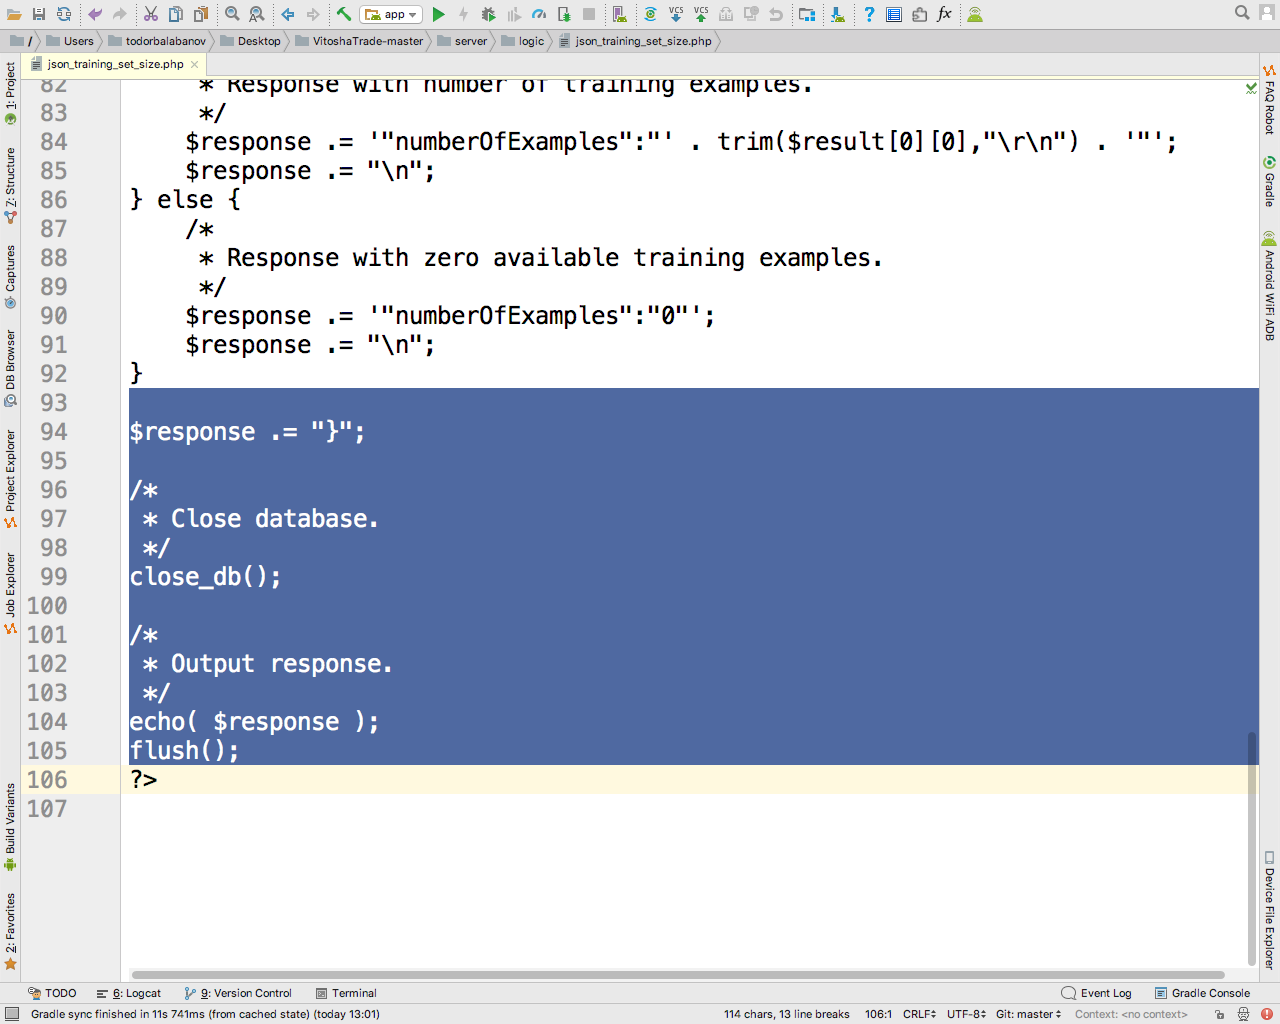
\includegraphics[height=0.45\pdfpageheight]{pic0141}
  \caption{Изпращане на отговор до клиента}
\label{fig:pic0141}
\end{figure}
\FloatBarrier

\subsection{Съхраняване на екземпляр изкуствена невронна мрежа}

Съхраняването на екземпляр от изкуствената невронна мрежа не връща резултат за изпълнението на операцията и поради тази причина не се използва JSON. След включването на модула за работа с базата от данни се изисква по-сложна проверка на входните аргументи, тъй като те са повече на брой и по-сложни (Фиг. \ref{fig:pic0142}-\ref{fig:pic0146}). 

\begin{figure}[h]
  \centering
  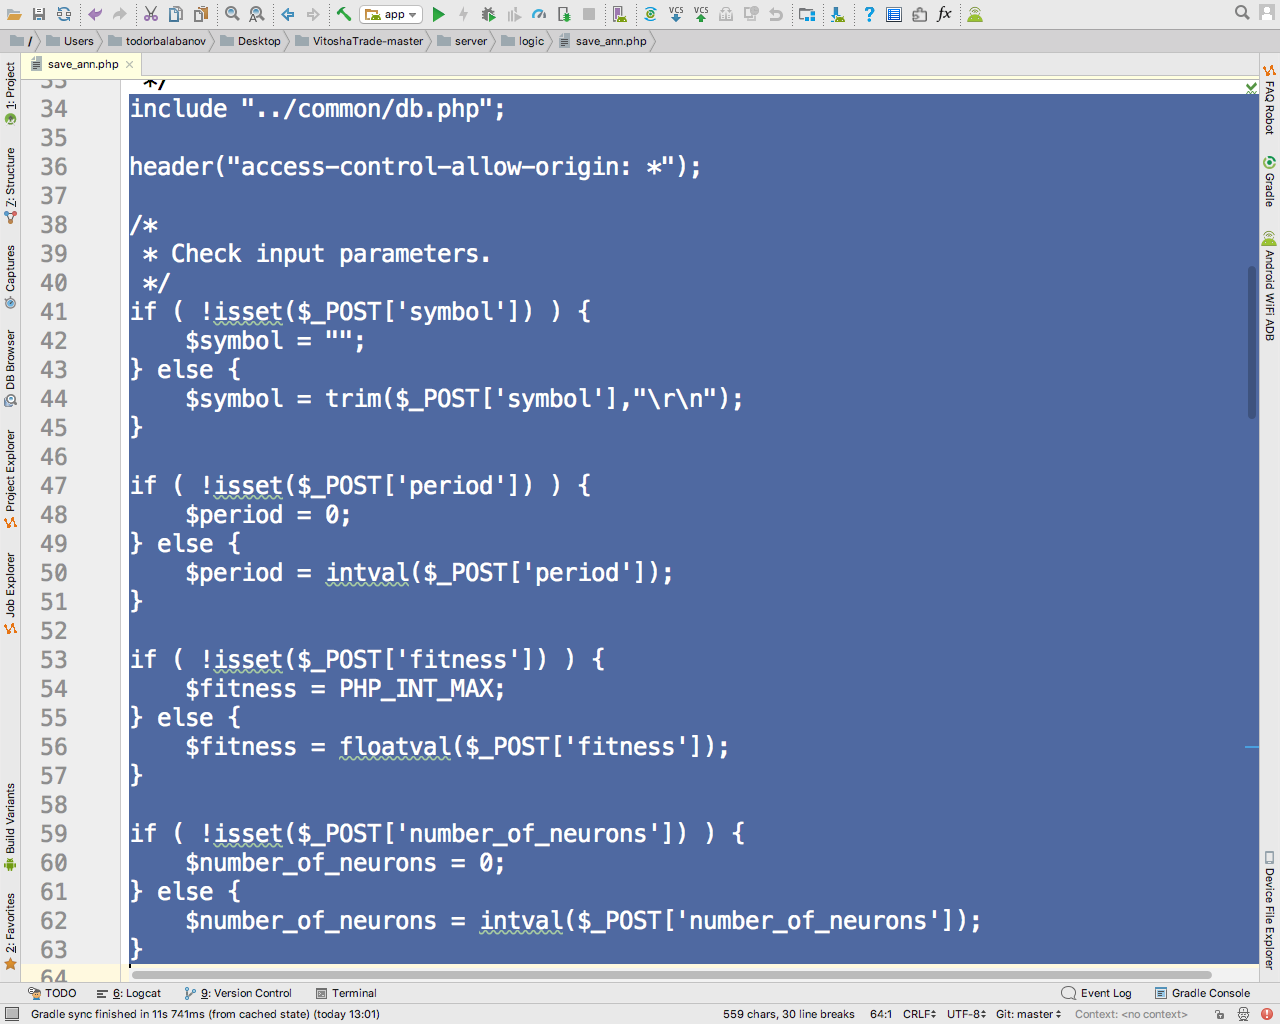
\includegraphics[height=0.45\pdfpageheight]{pic0142}
  \caption{Проверка на входните аргументи за валутна двойка, период, жизненост и брой неврони}
\label{fig:pic0142}
\end{figure}
\FloatBarrier

\begin{figure}[h]
  \centering
  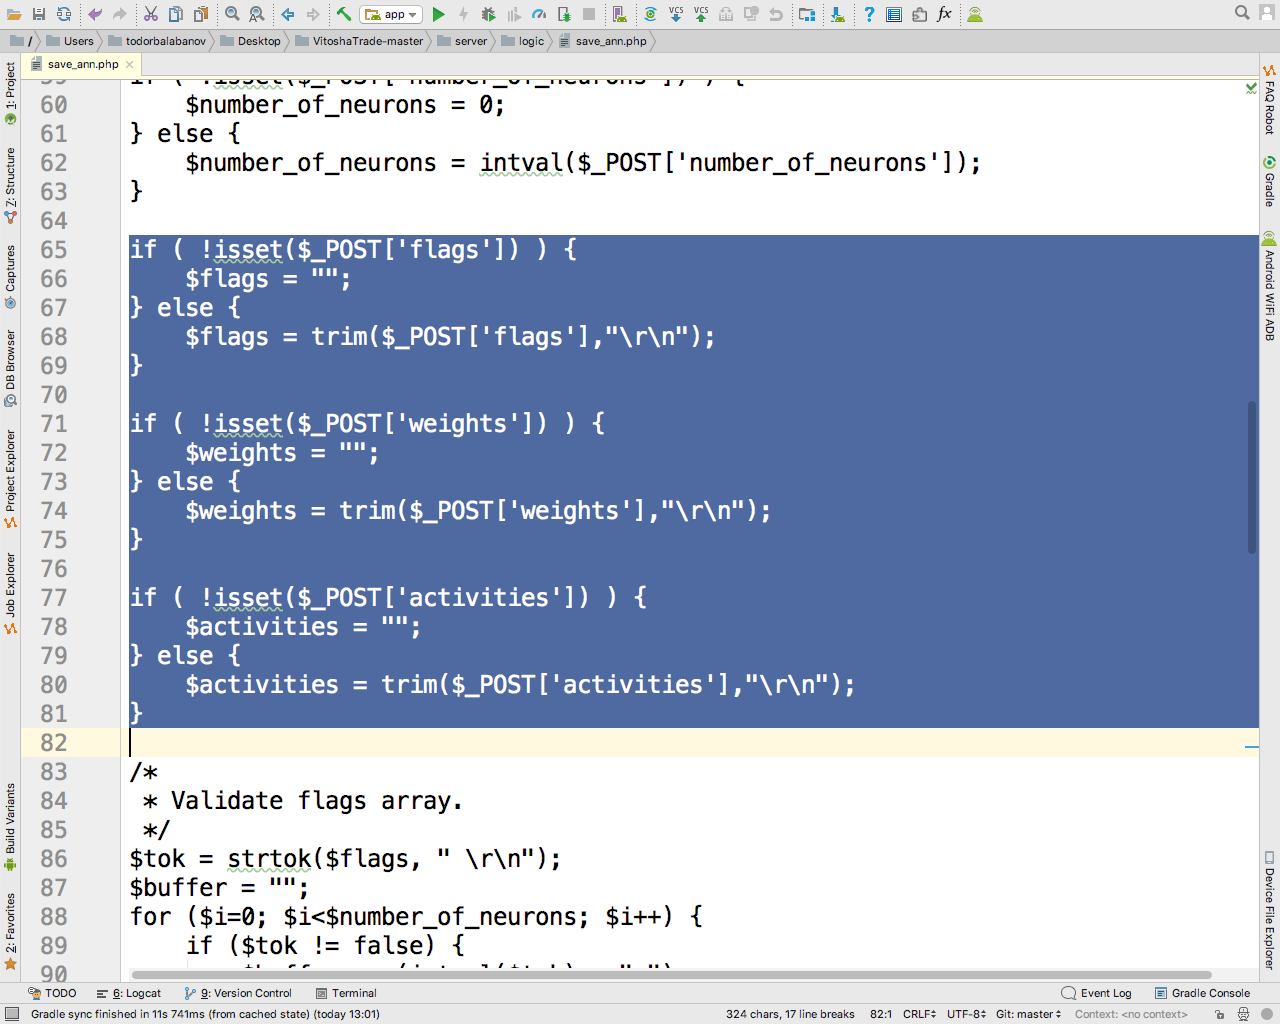
\includegraphics[height=0.45\pdfpageheight]{pic0143}
  \caption{Проверка на входните аргументи за флагове на невроните, връзки и тегла между невроните}
\label{fig:pic0143}
\end{figure}
\FloatBarrier

\begin{figure}[h]
  \centering
  \includegraphics[height=0.45\pdfpageheight]{pic0144}
  \caption{Проверка за типа на всеки неврон}
\label{fig:pic0144}
\end{figure}
\FloatBarrier

\begin{figure}[h]
  \centering
  \includegraphics[height=0.45\pdfpageheight]{pic0145}
  \caption{Проверка за стойността на всяко тегло}
\label{fig:pic0145}
\end{figure}
\FloatBarrier

\begin{figure}[h]
  \centering
  \includegraphics[height=0.45\pdfpageheight]{pic0146}
  \caption{Проверка за стойността на всяка връзка}
\label{fig:pic0146}
\end{figure}
\FloatBarrier

При този скрипт проверките са значително по-сложни, тъй като освен наличност на аргументите се следи за числените стойности, които пристигат от клиентското приложение. 

\begin{figure}[h]
  \centering
  \includegraphics[height=0.45\pdfpageheight]{pic0147}
  \caption{Съхраняване на екземпляр изкуствена невронна мрежа}
\label{fig:pic0147}
\end{figure}
\FloatBarrier

Същината на скрипта представлява отваряне на връзка към базата данни, изпълнение на съхранена процедура и затваряне на връзката към базата данни (Фиг. \ref{fig:pic0147}).

\subsection{Съхраняване на екземпляр изкуствена невронна мрежа след дообучение}

Когато определена изкуствена невронна мрежа е преминала допълнителен цикъл на обучение и бъде изпратена до отдалечения сървър, разумно е информацията да се съхранява само, ако води до подобряване на жизнеността. 

\begin{figure}[h]
  \centering
  \includegraphics[height=0.45\pdfpageheight]{pic0158}
  \caption{Проверка на жизнеността преди съхраняване на информацията}
\label{fig:pic0158}
\end{figure}
\FloatBarrier

Разликата между общата процедура за съхраняване на изкуствена невронна мрежа и съхраняването след допълнително обучение е в проверката на най-добрата постигната жизнена стойност (Фиг. \ref{fig:pic0158}).

\subsection{Съхраняване на тренировъчно множество}

По аналогичен начин, при съхраняването на тренировъчни примери не се връща JSON съобщение и кодът по проверката на входните данни превъзхожда кода за самото съхраняване. Първоначално се проверява наличието на аргументите (Фиг. \ref{fig:pic0148},\ref{fig:pic0149}).

\begin{figure}[h]
  \centering
  \includegraphics[height=0.45\pdfpageheight]{pic0148}
  \caption{Проверка на агументите за валутна двойка, период, брой примери и времеви маркери}
\label{fig:pic0148}
\end{figure}
\FloatBarrier

\begin{figure}[h]
  \centering
  \includegraphics[height=0.45\pdfpageheight]{pic0149}
  \caption{Проверка на агументите за отваряне, най-ниска стойност, най-висока стойност, затваряне и изтъргуван обем}
\label{fig:pic0149}
\end{figure}
\FloatBarrier

Всеки от масивите преминава допълнителна проверка за стойностите, които съдържа (Фиг. \ref{fig:pic0150}-\ref{fig:pic0152}).

\begin{figure}[h]
  \centering
  \includegraphics[height=0.45\pdfpageheight]{pic0150}
  \caption{Проверка на стойностите за времеви маркери и нива на отваряне}
\label{fig:pic0150}
\end{figure}
\FloatBarrier

\begin{figure}[h]
  \centering
  \includegraphics[height=0.45\pdfpageheight]{pic0151}
  \caption{Проверка на стойностите за най-ниско и най-високо постигнато ниво}
\label{fig:pic0151}
\end{figure}
\FloatBarrier

\begin{figure}[h]
  \centering
  \includegraphics[height=0.45\pdfpageheight]{pic0152}
  \caption{Проверка на стойностите за затваряне и изтъргуван обем}
\label{fig:pic0152}
\end{figure}
\FloatBarrier

Същинската част на скрипта отваря връзка към базата данни, изпълнява съхранена процедура и затваря връзката към базата данни (Фиг. \ref{fig:pic0153}).

\begin{figure}[h]
  \centering
  \includegraphics[height=0.45\pdfpageheight]{pic0153}
  \caption{Съхраняване на тренировъчно множество}
\label{fig:pic0153}
\end{figure}
\FloatBarrier